\documentclass{report}
\usepackage{setspace}
%\usepackage{subfigure}

\pagestyle{plain}
\usepackage{amssymb,graphicx,color}
\usepackage{amsfonts}
\usepackage{latexsym}
\usepackage{a4wide}
\usepackage{amsmath}

\usepackage[super]{nth}  % To format ordinal numbers e.g. 1st, 2nd, 3rd, 4th, etc.
\usepackage{enumitem}  % Remove spaces before an enumerate
\usepackage[style=ieee, sorting=none]{biblatex}  % BibTeX  
\usepackage{url}  % urls
\usepackage{listings}  % code snippets
\usepackage{longtable}  % tables
\usepackage{tabu}  % tables
\usepackage{textcomp}  % symbols

\newtheorem{theorem}{THEOREM}
\newtheorem{lemma}[theorem]{LEMMA}
\newtheorem{corollary}[theorem]{COROLLARY}
\newtheorem{proposition}[theorem]{PROPOSITION}
\newtheorem{remark}[theorem]{REMARK}
\newtheorem{definition}[theorem]{DEFINITION}
\newtheorem{fact}[theorem]{FACT}

\newtheorem{problem}[theorem]{PROBLEM}
\newtheorem{exercise}[theorem]{EXERCISE}
\def \set#1{\{#1\} }

\newenvironment{proof}{
PROOF:
\begin{quotation}}{
$\Box$ \end{quotation}}



\newcommand{\nats}{\mbox{\( \mathbb N \)}}
\newcommand{\rat}{\mbox{\(\mathbb Q\)}}
\newcommand{\rats}{\mbox{\(\mathbb Q\)}}
\newcommand{\reals}{\mbox{\(\mathbb R\)}}
\newcommand{\ints}{\mbox{\(\mathbb Z\)}}

\setcounter{secnumdepth}{3}  % Add numbering to \subsubsection
\setcounter{tocdepth}{3}  % Include \subsubsection in ToC
\setlist{nosep}  % Remove spaces before an enumerate
\setlength{\LTpre}{1em}  % remove spaces before longtable
\setlength{\LTpost}{0em}  % remove spaces after longtable
\newcommand{\textapprox}{\raisebox{0.5ex}{\texttildelow}}  % '~' sign

\bibliography{bibliography.bib}  % Load bibliography

%%%%%%%%%%%%%%%%%%%%%%%%%%


\title{{\vspace{-14em} 
\includegraphics[scale=0.4]{ucl_logo.png}}\\
{{\Huge Using Natural Language Processing (NLP) to develop a pipeline to analyse media representation of people with disabilities in Web-based news articles}}\\
%{\large Collection and filtering of online news articles, comparison of open-source sentiment models, and applications of the technology
%}\\
}
\date{Submission date: \nth{30} April 2018}
\author{Bagus Maulana\thanks{
{\bf Disclaimer:}
This report is submitted as part requirement for the MEng Degree in Computer Science at UCL. It is
substantially the result of my own work except where explicitly indicated in the text.
\emph{The report may be freely copied and distributed provided the source is explicitly acknowledged}}
\\ \\
MEng Computer Science\\ \\
Catherine Holloway, Nicholas C. Firth}



\begin{document}
 
\onehalfspacing
\maketitle
\begin{abstract}

\textbf{Report Title:}  Using Natural Language Processing (NLP) to develop a pipeline to analyse media representation of people with disabilities in Web-based news articles
%: Collection and filtering of online news articles, comparison of open-source sentiment models, and applications of the technology

\textbf{Author’s Name:} Bagus Maulana

\textbf{Supervisor’s Name:} Catherine Holloway, Nicholas C. Firth

\textbf{Date and Year of Submission:} \nth{30} April 2018\\
%% Three paragraphs:

%% What the project is about, the principle aims and goals, and specific challenges.
Research into the representation of groups (e.g. women, youth) in the news media is common across different research fields, from social sciences to computer science.
A common approach is to manually analyse a small sample of a few hundred news articles and generalise an overall conclusion from that sample. 
Computational Natural Language Processing (NLP) could be used to process articles much faster and vastly increase the sample size, which could uncover further information from a text corpus, such as trends i.e. how the conclusion varies over independent variables such as time.

%% How you carried out the project and what work it involved. How you went about meeting the project goals.
This project explores the feasibility of developing a computational pipeline that performs data collection from online news sources, filtering, parsing (feature extraction), sentiment scoring, statistical analysis, and data visualisation.
This pipeline is then used in an experiment to collect articles from three major British online news publishers and show trends regarding how the terms used and sentiment in news articles varies over time and between different publishers when reporting news related to disability or people with disabilities.

%% The results and achievements of the project. What the outcome is.
Results indicated that for some metrics, such as moving average of sentiment score, and on certain topics, minor trends over time and between different publishers are apparent, although inconsistent. 
While the approach showed promise in performing quantitative analysis upon large bodies of literature, and specifically in the media representation domain, it is highly recommended that future approaches to this media analysis problem improves upon this work by training a domain-specific filter and sentiment scorer with labelled data to improve the accuracy, and thus consistency, of sentiment scoring.

%% Half a page’s length.}
\end{abstract}
\tableofcontents
\setcounter{page}{1}


\chapter{Introduction} \label{Introduction} % 2-4 pages

%% Outline the problem you are working on, why it is interesting and what the challenges are.

% Talk about NLP
Natural Language Processing (NLP) encompasses a wide range of computational techniques for machine understanding of human (natural) language that are often used alongside each other.
The review article \cite{cambria2014jumping} defined Natural Language Processing as ``a theory-motivated range of computational techniques for the automatic analysis and representation of human language.''
The techniques that fall under the NLP umbrella include extracting term frequency distributions, text processing (e.g. tokenisation, stemming), part-of-speech tagging, text classification, information extraction (e.g. entity recognition), sentence structure parsing (parse tree), and sentiment analysis (or opinion mining) \cite{Nltk, liu2012sentiment}.
The computational models used in NLP range from simple rule-based models (e.g. counting words, or term frequency) to statistical machine learning and neural network models \cite{awesome-sentiment-analysis}. 
% Applications of NLP are used in everyday technologies, for example, information retrieval for search engines such as Google and Bing, and categorisation and topic modelling for recommendation engines used to suggest `similar' articles. % todo cite or remove

An advantage of NLP is that machines could process vast bodies of human-created literature (books, articles, posts, e-mails, messages, etc.) much faster than humans can, processing thousands of text documents per second. 
This allowed for high-level quantitative analyses of thousands or millions of text documents from a vast corpus to be feasible, which could uncover information previously inaccessible from manually reading only a small sample of documents and generalising from the sample.
This level of quantitative analysis could uncover trends and patterns from a text corpus, to answer questions such as ``How does the popularity of the term `mentally ill' increase or decrease year-on-year in British news media?'' 

% Other work in using NLP for media analysis
Applying computational NLP to perform meta-analyses over large text corpora has interesting potential applications in improving our understanding of the human world, such as analysing cultural trends quantitatively.
One study assembled a vast corpus of regional newspapers in the United Kingdom spanning 150 years to detect long-term patterns of cultural change, such as the increase of female representation in the news, or the popularity of trains and horses for transportation \cite{lansdall2017content}. 
This was achieved by analysing trends for $n$-gram frequency (a count of words or phrases in a text document) and named entities (known people, organisations, locations, etc.) in text.

More specifically in the domain of media representation of particular groups of people (e.g. women, youth), several researchers have attempted to use features extracted using NLP to perform computational analytics of text, mainly from social media.
For example, a tool to classify racist and sexist posts in social media was developed by using NLP to extract $n$-grams and part-of-speech tags (labels of words corresponding to its definition and context, such as `noun' or `verb') from text posts \cite{waseem2016you}.
However, there is still a research gap in this area, especially for applying NLP for news articles, in the context of specific groups such as people with disabilities.
% Just give a short summary, expand this later in Chapter 2

% Why is it interesting & what the challenges are
The representation of groups such as people with disabilities in media has been a popular research theme in social science.
For example, a 2002 study analysed a sample of 600 print articles relating to mental illnesses in New Zealand to measure the proportions of positive and negative depictions and predominant themes (e.g. criminality, educational accomplishments) \cite{coverdale2002depictions}.
There were attempts to discover trends, such as a study conducted in 1998 \cite{gold1999media} and replicated in 2008 \cite{devotta2013representations} which assessed change in representations of disability and people with disability in Canadian news media.
However, the study provided only two data points (1998 and 2008) with relatively small sample sizes of 196 news articles in 1998 and 166 news articles in 2008.

Applying computational NLP to this field would allow the possibility of discovering higher-level trends, by computationally analysing a much larger sample of articles, then identifying trends by creating subsets based on independent variables such as year of publication and publisher.
In this research, a sample of 305,185 news articles (48,967 after filtering off-topic articles) from British online news sources were used.
However, challenges remain as contemporary syntax-based NLP approaches tend to be more limited in scope and are prone to inconsistencies (false positives and negatives), where mitigating these inconsistencies is currently an open area of research. % inconsistencies due to type-I and type-II errors? (false positives and negatives)
% Just give a short summary, expand this later and give more papers in Chapter 2

%% List your aims and goals. An aim is something you intend to achieve (e.g., learn a new programming language and apply it in solving the problem), while a goal is something specific you expect to deliver (e.g., a working application with a particular set of features).
The aim of this project was to show the feasibility of utilising computational NLP approaches to perform a meta-analysis of literature available in the public online news media.
More specifically, to collect news articles relating to people with disabilities in British online media, and perform analyses using NLP at scale to identify trends such as term popularity and variations in positive/negative sentiment over variables such as date published and publisher.

This project's goals were to achieve the stated aim by developing a computational pipeline capable of performing analysis on online news media in full, from data collection to analysis and visualisation.
Given a list of topics related to disabilities, each topic consisting of key terms and query terms, which can either be a single word i.e. a keyword, or a sequence of words i.e. a key phrase;
this pipeline accomplished the tasks of: 
web crawling and scraping web sites to collect a dataset of news articles;
filtering relevant articles given key terms; 
extracting relevant sentences that referred to a key term from these articles;
scoring the sentiment of these sentences;
and producing relevant visualisations and statistical analyses to show trends.
This pipeline is available open source on GitHub (\url{https://github.com/bmaulana/nlp-media}).

The main NLP techniques that were relevant for this project are:
text processing, to parse text and other relevant information from web news articles, and `prepare' text for further analyses using tokenisation (splitting text into a list of tokens, or words) and stemming (reducing words to their word stem, e.g. talked \textrightarrow\space talk);
term ($n$-gram) frequency, to quantitatively count the occurrence of words and phrases (sequences of words) in an article;
sentiment analysis, to produce a `sentiment score' of news articles that correspond to its perceived positive/negative view.
These techniques were implemented by utilising open-source NLP implementations.

%% Give an overview of how you carried out the project (e.g., an iterative approach).
This project was carried out in a modular approach. The pipeline was developed as individual components: 
a web scraper and crawler for data collection given a list of queries; 
a filter to remove irrelevant articles given a list of key terms; 
a parser to extract term occurrences and relevant sentences from articles, given a list key terms; 
a sentiment scorer for sentences and articles; 
and a script to perform statistical analysis on the results and produce relevant plots. 
A main pipeline script connects these components together by calling them in sequential order, performing analyses for each topic and Web news source (Daily Mail, Daily Express, Guardian).
This approach was ideal as changes could be made to a component without affecting or needing to rewrite code in other components.
Each component's output is saved to a JSON \cite{rfc8259} file, and the next component reads the previous component's output file, which ensured that computation can be `resumed' without recomputing the previous component. % is this too much implementation details for intro? meant to show advantages of modular approach

%% A brief overview of the rest of the chapters in the report (a guide to the reader of the overall structure of the report).
The body of this report is subdivided into four chapters, followed by a conclusion and appendices.
Chapter \ref{Context} covers related work on the domain of news media analysis (especially in the context of people with disabilities), a background of NLP research, and information regarding the relevant technologies researched for this project.
Chapter \ref{Requirements and Analysis} defines a structured list of requirements, goals, and expectations for this project.
Chapter \ref{Design and Implementation} documents the design and implementation of the computational pipeline and its components that were used to carry out the data analytics experiment and achieve the stated goals.
Chapter \ref{Results Evaluation} discusses the experiment's results in diagrams, graphs, and tables.
Finally, the conclusion, Chapter \ref{Conclusions}, evaluates the project, summarises key achievements and takeaways, provides recommendation on how this work could be expanded upon, and sets guidelines for further work in this field.
Furthermore, the bibliography lists sources that were used as references in this project, and the Appendix section contains the raw results of the experiment, including graphs and data not in Chapter \ref{Results Evaluation}.

% Brief results & conclusions
The performance of several open-source sentiment analysis implementations were compared to judge their suitability for the sentiment scoring task, given the domain of sentences from news articles related to disabilities or people with disabilities.
Results indicated that a relatively simpler rule-based model, VADER \cite{VADER}, outperformed more complex supervised machine learning or neural network models, which had been trained on other domains, such as tweets and IMDb/Amazon reviews, and proved to be less generalisable for this domain.

This project proved the feasibility of utilising NLP-based technologies to derive trends from a large corpora of online news articles relating to disabilities or people with disabilities.
The results showed that, for example, the perceived sentiment of Guardian articles are, on average, significantly higher than Daily Express and Daily Mail articles for the topic `disabled'.
It also showed an decreasing trend over time on the use of `invalid' and `handicap(ped)', and an increasing trend for `accessibl(e)', within Guardian articles.

These results could have a substantial impact on how research should be conducted for similar studies on the media's representation of groups of people, as it showed that NLP could be used to analyse a much larger sample of text documents than traditional approaches and derive meaningful trends.
However, challenges remained due to the sentiment scorer's inaccuracy.
The accuracy and consistency of results could be further improved in future work by developing a domain-specific supervised model for filtering and sentiment scoring, trained on an adequately-sized labelled dataset of news articles within the domain.   

%% This chapter is relatively short (2-4 pages) and must leave the reader very clear on what the project is about and what your goals are


\chapter{Context} \label{Context} % 8-10 pages

%% This chapter should cover background information, related work, research done, and tools or software selected for use in the project.

%% Provide necessary context and background information to describe how your project relates to what is already known or available.

%% A description of the research carried out to learn out about the nature of the problem(s) being investigated and potential solutions. The form of the research will vary widely depending on the kind of project. For example, it might involve searching through research publications and online resources, or might involve an exploration of design possibilities for a user interface or program structure.

%% The sources of information you are drawing on (papers, books, websites, etc.) should all be cited or referenced clearly. In addition, state how each source relates to your work and avoid the temptation to pad out the chapter by including sources that you didn’t make use of during the project.

%% If relevant, a survey of similar solutions, programs or applications to yours, and how yours is differentiated.

%% Introduce the software, programming languages, library code, frameworks and other tools that you are using. Discuss choices and make clear which you made use of and why.

%% You should not include well known things (e.g., HTML or Java) or try to give tutorials on how to use a tool or code library (use references to books and websites for that information). Everything you include should be directly relevant to your work and the relationship made clear. This chapter is likely to be fairly substantial, perhaps 8-10 pages.

% -- How the project relates to what is already known & available, survey of similar solutions --
\section{Background} \label{Background}  % 3-4 pages

% Similar research being done on media representation of (disability/mental illness/etc.).
Analyses of news media has been a popular research method.
News media provides an overview of the prevailing society's conceptions or views regarding a theme or topic, which can be analysed to deduce quantitative information.
This approach has been commonly used to study representations of particular groups of people, such as women, youth, or people with disabilities, as the language used in the media reflected and shaped prevailing views, and had been shown to differ (with statistical significance) in different societies.
For example, it was shown that the Canadian press was more likely to name individuals with disability and use appropriate labelling than the Israeli press in 1998 \cite{gold1999media}.
Furthermore, there is evidence to suggest that news media sources contribute to shape and reinforce beliefs among the society, such as misconceptions and stigma \cite{wahl1992mass}.

There had been various studies related to the public awareness of disabilities.
% While not necessarily related to news media,
A review in 2011 \cite{scior2011public} found 75 articles and 68 studies that passed a selective inclusion criteria with regards to intellectual disabilities, published in English between 1990 and mid-2011. 
Their inclusion criteria omitted studies which were found to be irrelevant, duplicate, or not written in English; and only accepted articles which were published in full in peer-reviewed journals, and the study's subject had to be the general public of working age (instead of particular subgroups).
This showed interest within the research community to find new ways to understand and quantify the public's perception towards disabilities.
% The topics brought up include the public's knowledge, attitudes, and beliefs about intellectual disability; and varying for socio-demographic characteristics, cross-cultural comparisons, and the effects of interventions.

Analyses of news media were primarily carried out by obtaining a small sample of documents (news articles) from a text corpora, such as all news articles published in England for a certain period, and analysed them manually. There had been various such studies on news media within the domain of disability representations:
\begin{itemize}
	\item In a 2002 study \cite{coverdale2002depictions}, researchers analysed a sample of 600 print articles published in New Zealand relating to mental health or mental illness that were collected by a commercial clipping bureau.
		The articles were categorised into positive or negative depictions; and further into themes such as danger to others, criminality, vulnerability, etc.
		The study found that negative themes predominate about 3 to 1, with 27\% being positive.
		Given the study's scope, this conclusion cannot be generalised to learn trends of how the conclusion varies given certain variables such as time or location.
	\item A similar study in 2005 \cite{jones2009representations} analysed 1,515 articles relating to autism in Australian news media.
		All articles were read by two research assistants to ensure they are on-topic and then coded as either `negative' or `positive' in overall focus, and then coded into themes (e.g. funding, education, etc.).
		% Key findings include a relatively limited amount of helpful information, and a 'dual stereotype' of people with autism labelled as either dangerous and uncontrollable, or unloved and poorly treated. % is this relevant?
		% Relative to other similar studies, this study appears to be focused more on qualitative discussion compared to quantitative results. % is this relevant?
	\item A study conducted in 1998 \cite{gold1999media} and replicated in 2008 \cite{devotta2013representations} assessed change in representations of disability and people with disabilities in the Canadian news media.
		This study sampled 196 news articles in 1998 and 166 news articles in 2008.
		It found an increase in the usage of `person-first' terminology (e.g. person with disabilities) and a decrease in `disabling language' (e.g. disabled person). % is this relevant?
		This was an attempt to identify trends with regards to media representation of disability, however it only provided two data points (1998 and 2008) with relatively small sample size.
\end{itemize}

% Why using computational NLP will allow the discovery of more (high-level) information: trends, patterns, etc
Data collection and processing of text using computational techniques based on NLP are much more feasible in scale, cost, and time, relative to manual collection and reading of text. 
An automated script could be used to collect thousands of news articles published on the Internet per hour, a vast improvement over contracting a commercial clipping bureau to provide 600 articles as done in past studies \cite{coverdale2002depictions}.
By applying NLP-based computational techniques in analysing text, it would be possible to develop a pipeline that could analyse and extract quantitative information from news articles' text at a much faster pace than manual reading, enabling the analyses of a much larger scale of documents.

While a sample of few hundred documents was usually enough to provide statistically significant conclusions, by providing an analysis of the full corpora or a much larger sample, it would be possible to uncover additional information from the dataset.
Higher-level trends, such as how a conclusion varies by year, location, and publisher, could be discovered from a quantitative analysis of the larger dataset; by `splitting' the result set into smaller subsets based on independent variables such as year, location, and publisher, then comparing these subsets based on dependent variables such as term frequency.
Furthermore, computational pipelines for data collection and scoring news articles are more objective and reproducible than manual methods, which may vary due to each researcher's individual biases.

% Similar research on applying NLP for news media, social media, etc. in other domains - techniques & features they used, solutions they came up with, etc. - what could be applicable for this domain (sentiment relative to a certain topic)
There had been numerous attempts to take advantage of the NLP-based computational approach to conduct a more complete analysis of textual corpora. 
A team of researchers assembled a corpus of 35.9 million news articles from 120 publishers in the United Kingdom between 1800 and 1950, which represented 14\% of all news articles published in the United Kingdom over that period \cite{lansdall2017content}.
With a NLP-based computational approach, the researchers were able to extract quantitative time-series information, represented as $n$-grams and named entities, from the vast dataset, which allowed the researchers to discover macroscopic cultural trends. 
They analysed and compared $n$-gram trends across various topics and identified trends that reflect cultural shifts, such as `train' overtaking `horse' in popularity around 1900, or `labour party' overtaking `conservative party' and `liberal party' in news coverage from the 1920s.
Additionally, they used entity recognition to extract named entities, and identified trends based on known information about these entities, such as the proportion of female and male entities over time.
They also considered the geographical location of the publication, to identify how usage trends of $n$-grams such as `british' and `english' differ based on location.

The British news media study were inspired by prior discussions and studies on the potential of exploiting large text corpora to detect macroscopic, long-term cultural changes. 
A seminal study in 2011 \cite{michel2011quantitative} started the field of `culturomics', to perform large-scale quantitative analyses on text corpora.
In the seminal study, a corpus of 5 million digitised English language books published over 200 years, or about 4\% of all books ever published, were analysed to extract how often $n$-grams were used over time.
This data is available on \url{http://www.culturomics.org/}.
This information was then used to analyse trends in the English language: the size of the English lexicon, regularisation of English verbs from irregular to regular (`-ed') suffixes, or how quickly mentions of years (e.g. `1950') decline in use.
Influenced by the seminal study, numerous other studies adopted similar approaches to analyse large datasets: 
\begin{itemize}
	\item an analysis of 1.7 million Victorian-era books \cite{gibbs2011conversation}
	\item an analysis of 17,094 US Billboard Hot 100 songs between 1960 and 2010 \cite{mauch2015evolution}
	\item an analysis of a 3.9 million news articles sampled from the Summary of World Broadcasts (SWB) collection \cite{leetaru2011culturomics}
	\item an analysis of 2.5 million English-language news articles from 498 online news outlets from 99 countries \cite{flaounas2013research}
\end{itemize}
This approach had also been criticised for ignoring semantics and context.
For example, critics noted that ``thirteen hundred words of gibberish and the Declaration of Independence are digitally equivalent'' \cite{gooding2013mass}, issues with OCR quality and duplicate editions \cite{gooding2013mass}, or that the selection of digitised books were biased \cite{schwartz2011culturomics}.

There had been some progress in applying similar NLP-based approaches specifically in the domain of how specific groups of people are represented in the media:
\begin{itemize}
	\item An attempt to classify racist and sexist posts in social media, which used NLP to extract features (such as $n$-grams and part-of-speech tags) from social media posts, then used to annotate 6,909 tweets \cite{waseem2016you}.
	\item A study explored potential linguistic markers of schizophrenia in social media; using a dataset of 174 users with self-reported schizophrenia and up to 3,200 tweets per user, and a similarly-sized dataset of `control' (non-schizophrenic) users.
		The researchers used NLP to extract features based on lexicon-based approaches (i.e. a list of mental health related keywords), latent dirichlet allocation (LDA), Brown clustering, character $n$-grams, and perplexity from tweets, which were fed to a support vector machine (SVM) classifier \cite{mitchell2015quantifying}.
\end{itemize}
Despite these studies, there is still a visible research gap on applying computational NLP approaches with regards to the representations of specific groups, such as people with disabilities (or a specific disability).
This project focused on studying the representations of people with disabilities from online news articles.

% Research on relevant libraries, frameworks, etc.:
To date, advances in NLP research had made the `culturomics' approach much more feasible, efficient, and effective, even under limited time and hardware constraints.
A growing number of free and open-source tools for computational NLP and statistical analysis had been developed by the research community; including general NLP tools such as nltk \cite{Nltk}, SpaCy \cite{SpaCy}, and StanfordNLP \cite{StanfordNLP}, statistical analysis tools such as numpy \cite{Numpy}, scipy \cite{Scipy}, and scikit-learn \cite{Scikit-learn}, and data visualisation tools such as matplotlib \cite{Matplotlib}.
Section \ref{Technical Context} contains a further listing and discussion of these tools, alongside the specific libraries and NLP techniques used for this research project.

% -- Research carried out & sources (papers, books, websites, etc.) --
\section{Research Methodology and Sources} \label{Research Methodology and Sources}  % 1 page

% How background research was carried out
Background research was carried out by investigating papers from public sources such as Google Scholar.
Research articles were gathered from a list of important topics and query terms related to NLP, specific NLP techniques, disability, and news media: for example, `natural language processing review', `news media' AND `disability', `natural language processing' AND (`news media' OR `cultural trends'), `natural language processing' AND `disability', and `sentiment analysis'.
Highly-cited research articles were prioritised as examples, as they were deemed to be more `important' papers or studies within its topic.
Additionally, the author looked for highly-cited `key' papers and review articles within each specific topic, and consulted its list of citations (older papers) and research articles that cites the review article (newer papers) to expand the list of relevant research papers further.

% How technical research was carried out: for each component, determine neccesary or potentially useful techniques. Look up online for papers defining it, web resources, frameworks/libraries. Research done alongside development of code (do research as I plan/develop, which in turn may change how I'm doing things)
Technical research, on the other hand, was carried out as necessary.
After the requirements and components for the pipeline had been decided, research was carried out to find relevant techniques, formulae, algorithms, tools, libraries/packages, and existing implementations that would be useful to implement each necessary component.
This research was carried out in an iterative approach alongside software development. 
Initial planning and research would provide an initial implementation plan, the plan's implementation would uncover the feasibility of these approaches and possible alternatives/refinements to be researched, further research may reveal new options/refinements to be implemented, and so on.
Research or work done for a component may also reveal possible improvements and/or alternatives for another component, which may require further research and implementation.  
Again, more popular tools and libraries were prioritised; although several approaches and implementations were considered for most components and sub-tasks, to be compared for suitability, runtime, results, etc.

% Sources: Google Scholar, papers cited by other papers, GitHub pages, Python repositories (Pip, Conda), Python and library documentation, etc. + 'state how each source relates to your work'.
The sources that were used for this literature review are:
\begin{itemize}
	\item Google Scholar, often used to find research articles to act as `entry points' towards a research topic, to find other studies similar to a research article, or to retrieve citation information with regards to research paper, book, or popular Python package.
	\item GitHub topics, used to find repositories that are relevant to help implement a specific NLP technique or component, find similar/alternative implementations, and was also used as a benchmark for the popularity and range of solutions for a topic in a given programming language.
	\item Several GitHub pages also curate a list of repositories for a specific topic \cite{awesome-sentiment-analysis, awesome-nlp, awesome-machine-learning}.
	\item Python package repositories such as PyPi \cite{PyPi} and Anaconda Cloud \cite{Anaconda-Cloud}, which listed all available Python packages, provided general information regarding them, and a search function; useful to find relevant packages for a component/task and gather information about a Python package.
	\item Official web sites and documentation of Python packages, which listed and defined the capabilities of the package, used to explore a package's functionality and capacity to solve a specific task, and to understand the technologies and approaches used by the package's implementation. 
		On more popular packages, citation information regarding the package would often be available from its web site.
\end{itemize}

% -- Technical background, sources of information, software --% (probably the longest section in chapter 2)
\section{Technical Context} \label{Technical Context}  % 4-5 pages

% general NLP: define NLP again, classify & list techniques, then mention 'the techniques used in this project are ...'
Natural language processing (NLP), defined as ``a theory-motivated range of computational techniques for the automatic analysis and representation of human language'' \cite{cambria2014jumping}, encompasses a range of computational techniques to extract information from text.
In this project, NLP techniques were used to filter irrelevant articles, extract features such as relevant sentences from text, and score sentiment of articles, as defined in the project's goals.

Text processing was used by all components to `prepare' text for further analyses, where tokenisation was implemented to transform raw text into a list of tokens, and normalisation techniques such as stemming and stop word removal \cite{Nltk} were used to remove the distinction between equivalent tokens.
Dataset filtering was implemented by measuring term frequency, or counting words and phrases (sequences of words), for each article.
Feature extraction was implemented by using a rule-based matcher to find occurrences of tokens that refer to key terms.
Sentiment scoring was implemented using a selection of open-source sentiment analysis tools, which were compared based on their accuracy on a small, manually-labelled sample of the dataset.

Not every component defined in the project goals required NLP techniques.
Data collection was performed using established general-purpose tools for sending web requests and scraping text from web sites.
Similarly, statistical analysis and data visualisation was performed using general purpose statistical and data visualisation tools.
This section covers the technical tools that were researched for all components of the solution, and the alternatives that were considered, regardless of whether NLP was utilised.

NLP covers three main `curves' or areas: syntax, semantics, and pragmatics (narratives, understanding) \cite{cambria2014jumping}. 
Syntax specifies the way symbols and groups of symbols are arranged and whether they are well-formed in an expression, whereas semantics specifies what these expressions mean, and pragmatics specifies contextual information.
Contemporary approaches to NLP mainly focus on syntactic analysis, due to the relative ease of extracting syntactic features of text, such as term frequency and part-of-speech tags.
However, syntactic analysis is much more limited, as it often misses information about the semantic context of a word.
For example, the distinction between the word `one' in ``there's no one there'' (referring to a person) and in ``we have only one car'' (referring to a quantity) is lost.
This report focuses on syntactic techniques and features, as these are more relevant to the necessary text processing, filtering, feature extraction, and sentiment analysis techniques that are feasible with current technology at this scale.

% Programming language: written in Python
Python 3.6.3 \cite{Python} was used as the main programming language for this project.
It was chosen for the extensive availability and range of Python tools for NLP, sentiment analysis, statistical analysis, data visualisation, web scraping and parsing, etc.
A study in 2016 showed that Python is the most popular language for machine learning and data science \cite{puget2016most}.
A GitHub search for the topic `nlp' as of 18 April 2018 reported 1,397 Python and 470 Jupyter (a Python-based interactive `notebook' technology) repositories with the tag `nlp', compared to the second most popular programming language being Java with only 251 repositories tagged with `nlp' \cite{GitHubNLP}.
Furthermore, Python is an ideal language for quick experimentation due to the relatively high level of abstraction and low verbosity of Python code, which makes it relatively easier to make changes on the fly.
The Anaconda distribution of Python \cite{Anaconda} was used due to its suitability to set up and manage Python environments and packages for data science projects.

\subsection{Data Collection Methods} \label{tc-data-collection}
% Data collection
General-purpose tools for sending HTTP requests (to open web addresses/URLs and store HTML web pages programmatically) and parsing HTML code (to parse article text and metadata from raw HTML web pages) were sufficient for data collection.

The Requests library \cite{Requests} is a popular Python tool with 400,000+ daily downloads for sending HTTP/1.1 requests.
A HTTP GET request retrieves the HTML code, alongside other information, associated with a given URL from a web server, similar to opening the page on a web browser. 
Requests stores the web server's response, including the HTML code, as a Python object.

BeautifulSoup \cite{BeautifulSoup} is a Python library that provides simple functions to navigate and search a parse tree, such as HTML code.
As the web pages of online news articles from the same source/publisher tend to follow a similar HTML structure, BeautifulSoup could be used to parse article text and relevant metadata such as headline and date of publication, by searching for specific tags and attributes within the HTML code.
Similarly, BeautifulSoup could be used to parse outgoing links from a search page.

\subsection{Filtering Methods} \label{tc-filtering}
% Term frequency & filtering: mention 'tf ranking' & pre-processing (stemming)
In this project, filtering of off-topic articles were achieved by measuring the term frequency of key terms independently for each document.
Term frequency (tf) is a simple and commonly-used metric in NLP, with various existing tools that can compute this metric for thousands of text documents per second.
To put simply, the frequency of a term (a token or sequence of tokens) in a document is the number of times that the term occurs in the document.
The popular scikit-learn library \cite{Scikit-learn} provides a tool (CountVectoriser) to measure term frequency of all tokens (words) in a corpus of text documents, handling the tokenisation of raw text (converting a raw text document into a list of tokens) and counting token occurrences.

For text normalisation, CountVectoriser provides the option to ignore stop words, or common words in English which do not add topical information, such as `the' and `a', which can often bias results due to their relatively high occurrences.
Additionally, the nltk library \cite{Nltk} was used for `stemming': to reduce all words in the document to its word stem, such that e.g. `walk', `walks', `walked', and `walking' are equivalent.
Furthermore, all text in the article were converted to lower-case to ignore capitalisation, such that e.g. `disability' and `Disability' are equivalent.

In literature related to NLP, more complex approaches had been proposed and used for the task of text classification and filtering off-topic articles.
A conventional approach is by calculating term frequency --- inverse document frequency (tf-idf) \cite{robertson2004understanding, sparck1972statistical}, a metric that builds on term frequency by considering the relative importance of each word.
Inverse document frequency (idf) is calculated by counting the number of documents in a corpus where a term appears: if a term appears more frequently, it is deemed to be less important and assigned a lower score.
For example, common words such as `the' are assigned very low idf scores.
The tf-idf score is measured by multiplying tf with idf.
However, this approach was not suitable for this project, given the selective nature of the corpus, as only articles containing defined query terms were collected; thus the idf scores of these query terms were be flawed, as at least one query term would exist in every document.

Another often-proposed approach was to use a supervised machine learning model to classify documents into pre-defined categories (the text classification problem).
Various supervised machine learning models were proposed to solve text classification, including Support Vector Matrices (SVM), Na\"{i}ve Bayes (NB), and k-nearest neighbour (kNN) models \cite{khan2010review}.
However, this approach was not feasible for this project due to a lack of labelled data, i.e. a dataset of articles with ``is this article relevant?'' labels.

Topic models, which computes the proportion of abstract `topics' in a document, had also been proposed.
Latent dirichlet allocation (LDA) \cite{blei2003latent} represents documents as random mixtures over latent topics, where each topic is characterized by a distribution over words.
However, as these topics are abstract and characterized generatively (each topic's distribution over words are generated by the model, rather than pre-defined), it is not very useful for the task of classifying whether a document matches pre-defined key terms.
Additionally, LDA is significantly more computationally expensive than tf or tf-idf.

\subsection{Feature Extraction Methods} \label{tc-matching}
% Rule-based matching to find sentences relevant to one or more keyword(s) or key phrase(s)
% match similar sentences if it contains a phrase that has the same lemma (root word) as the keyword or key phrase (in the same order), for example, 'Mental illnesses' will match 'mental illness'
% Cite SpaCy, 'used SpaCy to perform rule-based sentence matching'
Before the sentiment scores of news articles could be measured, the sentences that are relevant to each topic, given a list of key terms, had to be extracted from the article's text.
This required NLP tools to parse text and extract structural information, such as sentence structure.
Other features, such as the frequency of each key term on each article, could also be extracted while parsing text.

SpaCy \cite{SpaCy} is a popular Python library for parsing raw text.
It handles the tokenisation and normalisation of raw text, and extracts information such as part-of-speech tags and named entities, using pre-trained convolutional neural network models.
SpaCy was benchmarked to be the fastest and among the most accurate syntactic parser, being able to parse 13,965 words per second in 2015 \cite{choi2015depends}.

Among the information SpaCy extracts from text are lemmas, or word stems, of all tokens (e.g. `mentally' \textrightarrow\space `mental').
SpaCy also features a rule-based matching engine, which retrieves a list of tokens or sequences of tokens within a document that matches a given pattern, such as tokens with a specified lemma, or sequences of tokens with a specified sequence of lemmas.
This was used to implement the task of extracting relevant sentences from an article, defined as sentences containing a word (token) or phrase (sequences of tokens) equivalent to a key term.

\subsection{Sentiment Analysis Methods} \label{tc-sentiment}
% Sentiment analysis: cite some survey papers, cite GitHub page, cite each library I tried (this would probably be the longest section)
Sentiment analysis, or opinion mining, was defined as ``the field of study that analyzes people's opinions, sentiments, evaluations, attitudes, and emotions" from natural language \cite{liu2012sentiment}.
A GitHub search for the topic `sentiment-analysis' as of 18 April 2018 reported 450 Python and 222 Jupyter repositories with the tag `sentiment-analysis' \cite{GitHub-sentiment-analysis}.
Furthermore, there exists a community-curated list of sentiment analysis implementations on GitHub \cite{awesome-sentiment-analysis}, which served as a useful starting point to explore open-source sentiment analysis implementations.

A variety of open-source tools and pre-trained models dedicated to sentiment analysis were researched for the purpose of comparison.
Except for VADER and TextBlob's PatternAnalyser, these models were based on supervised machine learning or neural network approaches, which infers patterns between features (information extracted from text using NLP) and labels (sentiment scores) from a labelled training dataset, and uses these learned patterns to estimate the label of `unseen' text.
However, patterns learned from other domains (e.g. social media posts) may not be fully relevant in the domain of this experiment (news articles related to disabilities).
On the other hand, VADER and TextBlob's PatternAnalyser implement a relatively less complex rule-based model, which computes sentiment scores based on the presence of pre-defined rules or patterns.
Unless otherwise stated below, these tools all return a real-valued sentiment score between -1.0 and 1.0 for each sentence.

The particular sentiment analysis implementations that were explored in this paper are:
\begin{itemize}
	\item VADER \cite{VADER} is a relatively simple rule-based model that scores the sentiment of a given sentence based on rules such as: the presence of `sentiment lexicons', a list of lexical features common to sentiment expression, such as `good' and `bad', including slang words, emoticons, and acronyms; negations (e.g. `not good'); and `emphasis', or increased sentiment intensity due to punctuation, capitalisation, and degree modifiers (e.g. `very').
	\item xiaohan2012's `twitter-sent-dnn' repository provides a trained convolutional neural network model with dynamic k-max pooling (DCNN).
		The model considers features based on word and $n$-gram order of the sentence, and an induced feature graph generated by the DCNN.
		It was trained on a dataset of 1.6 million tweets with inferred labels based on emoticons.
		It is an implementation of \cite{kalchbrennerACL2014}.
	\item kevincobain2000's `sentiment\_classifier' repository \cite{kevincobain} provides a trained supervised machine learning model based on Na\"{i}ve Bayes and Maximum Entropy Classifier, which transforms a sentence to positive and negative sentiment scores.
		It uses bigrams (a 2-gram, sequence of 2 adjacent words) as features, implements Word Sense Disambiguation using wordnet \cite{banerjee2002adapted} to tranform bigrams to `senses', and considers word occurrence statistics from nltk's movie review corpus.
		Its training data is a mixture of nltk's movie review corpus, Twitter posts, and Amazon customer reviews data. 
	\item OpenAI's `generating-reviews-discovering-sentiment' repository provides a pre-trained single-layer multiplicative LSTM recurrent neural network model with 4096 units, a relatively simple model optimised for training/convergence time.
		It was trained on a dataset of over 82 million Amazon product reviews from May 1996 to July 2014, a substantially larger training set than any previous work, and outperforms state-of-the-art models when tested on similar-domain corpora such as Rotten Tomatoes and IMDb reviews.
		Sentences are represented as a sequence of UTF-8 encoded bytes, used as features. 
		% For each byte, the model updates its hidden state and predicts a probability distribution over the next possible byte. 
		It is an implementation of \cite{OpenAI}.
	\item Stanford CoreNLP \cite{StanfordNLP} provides a set of linguistic analysis tools, including sentiment analysis, running in a local server.
		Its sentiment analysis tool uses a recursive neural network model, converts sentences to parse trees to be used as features, and were trained on a dataset of fully-labelled parse trees for 215,154 unique phrases and 11,855 sentences from the Rotten Tomatoes movie review corpus. 
		Unlike other scorers in this list, it classifies sentences into five sentiment classes, from `very negative' to `very positive', instead of assigning a real-valued score. \cite{socher2013recursive}.
		Although Stanford CoreNLP was written in Java, several packages exist that allow a Stanford CoreNLP local server to be started and queried programmatically in Python \cite{stanfordcorenlp}.
	\item TextBlob \cite{textblob} is a general-purpose NLP library similar to nltk, SpaCy, or CoreNLP.
		It provides two sentiment analysis models: PatternAnalyzer, a rule-based classifier based on part-of-speech pattern matching, and NaiveBayesAnalyzer, a Na\"{i}ve Bayes classifier trained on a dataset of movie reviews (with no information on features used or dataset size). 
\end{itemize}

Several other repositories were also explored, however deemed unsuitable for this project either due to requiring labelled training data, which were unavailable for the domain of news articles relating to disabilities, instead of providing a pre-trained model, or the implementations are broken or infeasible.

\subsection{Statistical Analysis and Data Visualisation Methods} \label{tc-visualisation}
% Statistical analysis: matplotlib, papers (or at least a link to matplotlib's docs) for each statistical tool used (mean, standard deviation, scatterplot, moving average, 2d histogram, box and whiskers plot, violin plot, Mann-Whitney U test, etc.)
For statistical analysis and data visualisation, the conventionally used libraries in Python are numpy \cite{Numpy}, scipy \cite{Scipy}, scikit-learn \cite{Scikit-learn}, and matplotlib \cite{Matplotlib}.

Numpy \cite{Numpy} provides a powerful and efficient $n$-dimensional array object (often required for other libraries).
It provides efficient functions that perform mathematical computations over real values, vectors (1-dimensional arrays), and matrices (2-dimensional arrays) such as scalar/vector/matrix addition and multiplication, extracting a vector from a matrix's column, and boolean filtering.
Numpy is efficient as its functions are a Python wrapper for functions written in C, which allows for more direct hardware-level access than pure Python \cite{Numpy-c}.

Scipy \cite{Scipy} is a library that extends numpy to provide additional domain-specific functions. It extends numpy's 2-dimensional array to implement a sparse matrix, which only stores non-zero values in memory, useful in cases of a very large matrix where most elements are zero; such as a term frequency matrix of `all tokens' $\times$ `all documents' where most documents only contain values for a very small subset of tokens.
It also provides implementations of statistical equations, such as the Mann-Whitney $U$ Test used to compare subsets of data, defined below. 

Scikit-learn \cite{Scikit-learn} provides efficient implementations of algorithms for data analysis, feature extraction, and machine learning, built on top of numpy and scipy.
In this project, scikit-learn was used for data processing, such as the CountVectoriser used to compute term frequencies.

Matplotlib \cite{Matplotlib} is a 2D plotting library that produces visual graphs from lists/arrays.
It provides the capability to generate various types of plots, such as scatterplots, line plots, histograms, and box-and-whisker plots.
Furthermore, matplotlib's plots are very flexible, as parameters such as colours, labels, and bounds could be modified, and a legend or colour bar could be generated.
It also allows to concatenate plots in a grid of subplots, and plot multiple graphs in the same axes.

The types of plots and statistical metrics that were deemed relevant in this project are:
\begin{itemize}
	\item Scatter plot, used to show the distribution of data within two variables (e.g. year published and sentiment score). 
		Colour could be added to show a third variable (e.g. source/publisher of article).
		Available on matplotlib.
	\item Histogram (and two-dimensional histogram), used to show the distribution of articles relative to variables such as publisher, year of publication, and sentiment score ranges. 
		Available on matplotlib.
	\item Box-and-whiskers \cite{tukey1977exploratory} and violin plot \cite{hintze1998violin}, also used to show and compare the distribution of dependent variables (e.g. sentiment score) within different subsets of the data separated by independent variables (e.g. publisher).
		Available on matplotlib.
	\item Line graph, used to show trends in a dependent variable (e.g. sentiment score) over an independent variable (e.g. year of publication).
		Available on matplotlib.
	\item Mean and standard deviation, to quantify the distribution of articles within different subsets of the data separated by independent variables (e.g. publisher and year of publication) and provide a quantitative measure to compare different subsets.
		Available on numpy.
	\item Mann-Whitney $U$ Test \cite{mann1947test}, a non-parametric statistical test that measures whether it is true that given a randomly-selected value from a distribution, and another randomly-selected value from another distribution, the first value is equally likely to be less than or greater than the second value (i.e. there are no statistically significant difference between the two distributions), to show if the difference between two subsets are statistically significant.
		Available on scipy.
\end{itemize}

\chapter{Requirements and Analysis} \label{Requirements and Analysis}  % 5-6 pages

%% Give the detailed problem statement. This elaborates on what you may have included in the introduction chapter, and represents the starting point from which requirements were derived.
\section{Problem Statement} \label{Problem Statement}
% This project involves the development of a computational pipeline capable of performing data collection, natural language processing, statistical analysis, and data visualisation tasks

% Expand aims & goals
The primary aim of this project was to utilise available NLP-based technologies in order to perform a high-level meta-analysis of online news articles relating to people with disabilities available in the online British news media. 
The main objective was to reveal trends with regards to sentiment and word usage, by varying the dataset for independent variables such as source and date published.

The solution had to collect and scrape online news articles from the Internet, filter irrelevant articles, use available NLP-based tools to extract information from these articles, perform statistical analyses, and display visualisations of the data to show trends.
Of particular interest, as a dependent variable, was a sentiment (or opinion/polarity) index of articles (``how positively does an article view disabilities or people with disabilities?''), and how it varies given independent variables such as source and date published.
Thus, the general solution defined by this aim involved the completion of several sub-problems, primarily data collection, filtering, parsing, sentiment scoring, statistical analysis, and data visualisation.

To achieve this aim, the project's goals were to develop a computational pipeline that implements all components required for the general solution.
Before the project could be started, the topics relevant to this project had to be defined.
Thus, a list of topics relating to the domain of people with disabilities were compiled, each topic consisting of a list of key terms and query terms related to a specific disability, or disabilities in general.
Refer to section \ref{topics} for a list of topics, key terms, and query terms.

Given the list of topics, key terms, and query terms, the pipeline had to implement these following tasks (goals):
\begin{itemize}
	\item Web crawling and scraping web pages to collect a dataset of news articles, given the list of query terms for each topic.
	\item Filtering relevant articles from the dataset, given the list of key terms for each topic.
	\item Extracting relevant sentences that refer to a key term, from the dataset of filtered articles (feature extraction).
	\item Performing sentiment analysis (using open-source libraries and pre-trained models) on the dataset of relevant sentences.
	\item Producing statistical analyses and data visualisations to show trends over independent variables such as source and year published.
\end{itemize}

As the primary advantage of computational NLP is in its speed, and thus the vastly increased sample size that could be analysed relative to human reading, the solution must be able to collect and analyse the dataset quickly and at scale.
The total number of documents in the dataset, given the sources (section \ref{sources}) and query terms (section \ref{topics}) used in this experiment, was expected to number in the thousands to tens of thousands of documents per topic, or hundreds of thousands of documents in total across all topics.
Given this scale, the solution must be able to compute the full pipeline for the full dataset within a feasible timeframe of not more than a handful of days, given available consumer-grade hardware (Intel i7-6700HQ CPU @ 2.60GHz, NVIDIA GeForce GTX 1060 GPU) to show that the solution is feasible without specialised hardware.

%% A structured list of requirements.
\section{Requirements} \label{Requirements}

% Short paragraph about component based design
The solution followed a component-based design, where each task or goal must be implemented by a component that focuses only the specific task.
These components must be linked together via a main `pipeline' script that executes each component in sequential order, iterating through the full list of topics and sources.

This design was ideal as changes could be made to a component without affecting or needing to rewrite code in other components.
Additionally, each component's output was saved to a JSON \cite{rfc8259} file, and the next component reads the previous component's output file, which ensured that computation can be `resumed' without recomputing the previous component.

The list of required components were as follows: data collection, dataset filtering, feature and relevant sentence extraction, sentiment scoring, and statistical analysis and visualisation.

% Subsection for each component

\subsection{Data Collection} \label{req-data-collection}  % How to collect that data

% crawler finding articles from each source's built in search engines, look up multiple query terms
The data collection component must be able to find a list of news articles for each supported online source (Daily Mail, Daily Express, and Guardian), given a list of query terms related to each topic.
For each article, the only information required at this stage was a working URL pointing to an online resource containing the article text and relevant metadata.
Thus, the information that had to be provided by the component after this stage was a list of URLs pointing to relevant articles given a list of search queries.

% scraper for each source - what needs to be scraped from each article
After the list of URLs pointing to online news articles had been compiled, the component must be able to scrape these articles and extract the full article text and relevant metadata from each URL.
Aside from the full article text, the relevant metadata that must be extracted are the article's headline, URL, date of publication, and publication source.
The information must be returned in the form of an array of JSON objects, with each JSON object containing the text and metadata of a single news article.

This information must then be saved locally to a file where it could be read by the next component. 
The file and directory structure of the output file must be consistent given source and topic, such that the next component could find it programmatically.
This requirement holds for all other components in this pipeline.

% scalability, able to save and resume progress, etc.
As data collection was expected to consume the longest time compared to other components, due to the necessity to submit a web request for each article, additional requirements regarding scalability were enforced.
The data collection component must run in reasonable time (i.e. less than a day for each topic), given available hardware and a scale of up to tens of thousands of articles per topic.
Additionally, it should be possible to resume progress on data collection, such that it is possible to re-run the program at a later date to add new articles, without sending web requests for articles already in the collection.
It would also help in cases where the program is interrupted, Internet connection is lost, the machine is shut down, etc.
Thus, the component should immediately store already parsed articles to an external file, and read from the external file upon starting to gather a list of already saved URLs, and avoid re-parsing saved articles.

\subsection{Dataset Filtering} \label{req-filtering}

This component handled dataset filtering.
Initially, this component must be able to load the dataset of parsed articles, from the output file saved by the data collection component.
Each file contains a subset of all parsed articles for a specified topic and a specified source.

For each article, it must decide whether it is relevant to the topic defined by the subset, given a list of key terms related to each topic.
This decision should be based on the article's full text and headline, and should take all key terms associated with the current topic into account.
It should also be able to display a sample of an arbitrary number of articles, and the component's decision (on-topic/off-topic) for each sampled article, which would be used to analyse and improve the filter's accuracy.

The component must save all articles deemed on-topic (relevant to the topic) to a new output file, containing a list of JSON objects in the same format and retaining the same information as in the data collection component's output file.
Articles deemed off-topic (not relevant to the topic) must not be saved to the output file.

\subsection{Feature Extraction and Rule-based Sentence Matching} \label{req-matching}

This component parsed the article text using open-source NLP tools to extract relevant information required by the sentiment scoring and statistical analysis components.
Given the output file of the dataset filtering component, this component must be able to load the article text and metadata of all on-topic articles.

The sentiment scoring component required all `relevant' sentences relating to a key term (containing a keyword, key phrase, or an equivalent term) to be extracted from each article.
Thus, this component must extract all relevant sentences, as defined above, from all articles.

Additionally, the component should also extract other information as required by the sentiment scoring and statistical analysis components, including the total number of sentences and the number of relevant sentences in each article, and the term frequency of each key term in each article.

After these data had been extracted from each article, it must save the information to a new output file as a list of JSON objects, where each JSON object contains all the extracted information about a single news article, with a key for each extracted feature e.g. relevant sentences.
The metadata of each article (headline, date of publication, and source) must also be retained in the new output file, as they were required as independent variables for the statistical analysis component to analyse trends in the dataset.

\subsection{Sentiment Scoring} \label{req-sentiment}

The sentiment scoring component computed a real-valued sentiment score for each relevant sentence extracted by the feature extraction component.
This sentiment score which must correspond to the perceived `sentiment' of the sentence towards a disability, disabilities, a person with a disability or disabilities, or people with disabilit(y/ies), referred by the key term(s) in the sentence, with sufficient accuracy.
Given the output file of the feature extraction component, this component must be able to load the dataset of relevant sentences, and other data for all saved articles.

Two iterations of the sentiment scorer component must be developed.
The first iteration of the sentiment scorer component was used to perform a comparison between several open-source sentiment analysis implementations for this sentiment scoring task.
It was not used in the final pipeline.
The second iteration of the sentiment scorer component only computed one sentiment score for every sentence, using the best-performing sentiment scorer shown by the first iteration.
The second iteration was the one used in the final pipeline.

% Analysing scorers: 'slow' scorer that takes the first N articles only and scores them with ALL scorers from a list of open-source sentiment scorers, for the purpose of evaluating the performance (accuracy) of these scorers
\subsubsection{Comparison of Open Source Implementations} \label{req-sentiment-comparison}

The first iteration of the component must select an arbitrarily-sized sample of sentences from the dataset of relevant sentences.
Also, it must implement all open-source sentiment analysis implementations (`sentiment scorer') that were listed in section \ref{tc-sentiment}.

All sentences in the sample must be given a real-valued score between -1.0 and 1.0 by all sentiment scorers. 
The component should also allow the user to manually label these sentences as positive, neutral, or negative.
With this information, the component must be able to show the accuracy of each sentiment scorer, i.e. the proportion of true positives and true negatives, and show a confusion matrix.
It must also show the total, per-sentence, and per-article runtime of each sentiment scorer.

This iteration of the component was not used in the final pipeline, but only used as a tool to compare existing sentiment scorer implementations, and analyse their performance in the domain of news articles relating to disabilities or people with disabilities.

% Final product: one or two final sentiment scorers with only one sentiment score, optimised for performance (speed / runtime)
\subsubsection{Final Implementation} \label{req-sentiment-final}

The second iteration of the sentiment scorer component was the one used in the final pipeline.
It must only compute one sentiment score, using the best-performing sentiment scorer that runs in reasonable time, as shown by the results of the first iteration of this component.
It must compute the sentiment scores for all relevant sentences in the dataset (instead of only a limited sample of sentences).

After the sentiment scores of all relevant sentences within an article had been computed, this component must also compute the average sentiment score for each article.
Furthermore, the component must run in reasonable time (less than a day for each topic), given available hardware and a scale of up to tens of thousands of articles per topic.

After the sentiment scorer component had scored all relevant sentences and articles in the dataset, it must then save information about all articles, with score labels appended to each sentence and article, to a new output file.
The JSON objects of each article in the output file must retain the same format and information as the feature extraction component's output file, with the exception of an additional `sentiment score' key-value pair, within each sentence's and article's JSON object.

\subsection{Statistical Analysis and Visualisation} \label{req-visualisation}

The last component performed statistical analysis and data visualisation.
This component must read the sentiment scoring component's output files, to load the dataset of news articles and features extracted by previous components about each article.
At this point, information extracted about each article by previous components must include: source, publication date, and sentiment score, alongside other information.
To combine information about articles relating to the same topic from different sources, represented by different files, this component must be able to read multiple files in a single call, and collate the information into a single dataset.

This component must be able to show trends and visualisations that show how dependent variables (e.g. sentiment score) differ relative to the independent variables (e.g. publication year and source).
It should also compute statistical metrics to show whether the differences between subsets, as divided by the independent variables, are statistically significant.
The plot types and statistical metrics relevant to this analysis were defined in the end of section \ref{tc-visualisation}.

At a minimum, this component must visualise how sentiment score varies relative to publication year and source.
It should also show metrics related to distribution of sentiment scores on subsets divided by publication year and source.
Additionally, the component should also show visualisations based on information extracted by previous components other than sentiment scores, such as how the term frequency of each key term vary over time.

%% Use cases (a use diagram and list of use case titles, with the full use cases appearing in the appendix).
% Not applicable

%% Results of analysing the requirements to extract information. For example, data modelling to find the data to be stored (ER diagram), views/web pages needed and so on.
\section{Analysis of Requirements} \label{Analysis of Requirements}

% How the requirements influence the design of my project
The implementation design, and additional requirements of this project were highly influenced by the core requirements, i.e. data collection, filtering, sentence extraction, sentiment scoring, statistical analysis, and data visualisation.
The overall design of the pipeline, with isolated components for each sub-problem, stemmed from the largely independent tasks that were required to perform the data analysis experiment in whole, from data collection to analysis and visualisation.

Initial prototypes, or initial `runs' collecting only a limited number of news articles, showed that data collection used the majority of runtime.
For this reason, the requirement where it should be possible to resume progress on data collection, instead of repeating the process for already collected data, was added.

The JSON object formats for each component's output file were largely defined by the requirements of each component, i.e. the information that must be extracted by each component.
For example, the JSON object format of an article in the data collection component's output file is as follows:
\begin{lstlisting}
{
	"https://www.express.co.uk/comment/columnists/...": {
		"source": "Daily Express",
		"title": "Will she grow out of her stutter?",
		"datetime": "2008-02-12T00:00:00+00:00",
		"section": "comment",
		"subsection": "columnists",
		"text": "..."
	}
}
\end{lstlisting}
Where the URL and `source', `title', `datetime', and `text' fields correspond to requirements defined for the data collection component.

%% The level of detail of the requirements and use cases will depend on the nature of your project. If you are doing a Software Engineering based design and implementation project, then they will need to be done thoroughly. If there is a substantial body of requirements and use cases, then a summary should be given in the chapter, with the full set included in an appendix section.
%% If your project is not Software Engineering oriented, then you still need to describe the requirements you are working to and relevant analysis information. Use cases may not be needed or be relevant.
%% The analysis part of the chapter is what you did to map the requirements information into the first pass design. You can think of analysis as the first stage of design, and the purpose is to show how the requirements were used to inform the design. The length of this chapter depends on the kind of project, but you are typically looking at 5-6 pages.


\chapter{Design and Implementation} \label{Design and Implementation} % 10+ pages (use diagrams, graphs etc. to fill it up)

%% Describe the design of what you have created.
%% Start with the application architecture, giving its overall structure and the components that make up that structure.
\section{Overall Design} \label{Overall Design}

% Components, what each component does, how they interact with each other (show in diagram)
To fulfil the stated requirements in chapter \ref{Requirements and Analysis}, the solution that was decided is a computational pipeline that consisted of five main components.
This solution was used to carry out the experiment to collect and analyse online news articles and visualise sentiment trends over time and article source.
The results of this experiment are shown in chapter \ref{Results Evaluation}.

The high-level design of the pipeline and its main components were defined as follows:

\vspace{0.5em}
\noindent
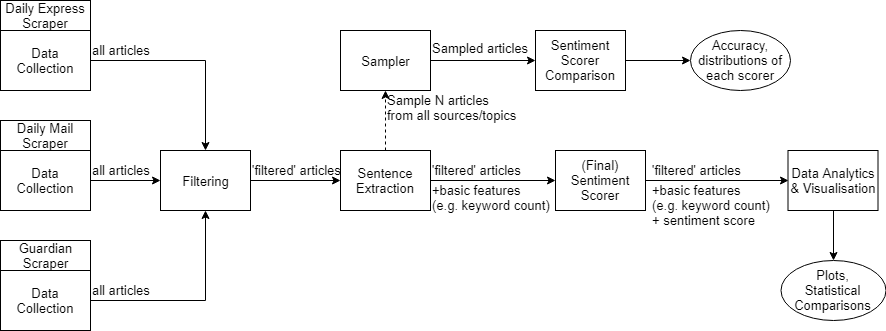
\includegraphics[width=\textwidth]{overall-design2.png}

In this experiment, the pipeline was ran once for each source and topic.
Each run up to the `sentiment scorer' component generated a dataset of all articles for the specified topic from the specified source, with all extracted features, stored in a file.
The `plot' component then loaded all files for every source within the same topic, and combined the datasets to produce visualisations that show trends within the topic, and computed statistical metrics for each possible subset within the topic.

% Input/output format (of JSON files) before/after each stage, how these files are stored (file structure and JSON structure)
Components passed datasets to each other by saving all information it extracts in a JSON file.
The output file of an earlier component is read as the input file for the next component, given the same source and topic.
The format of these files was a collection of JSON objects, where each line consisted of a single JSON object, and each JSON object represented a single article.
The JSON object contained a key-value pair for each extracted feature.
Each component retains information extracted by the previous components, while appending each object with additional key-value pairs for each feature it extracts.
This design ensures that in case computation is interrupted for any reason, the dataset generated by the previous component has already been saved to a file, and computation can restart from the interrupted component, without having to recompute previous components.

This modular design ensured that changes could be made to a component without affecting or needing to rewrite or recompute code in other components, which offered flexibility for experimentation.

%% Include the database or storage representation. (Originally after component description)
\section{Dataset Description} \label{Dataset Description}  % What data have I got

\subsection{Sources} \label{sources}

% sources (Guardian, DM, DE), why
The Internet is an increasingly common medium for news publishers to publish news articles, and for consumers to read news articles.
As of 2017, 64\% of British individuals read and/or download online news, newspapers or magazines; a sharp increase from 20\% in 2007 \cite{statista2018share}. 

The Daily Mail (\url{dailymail.co.uk}) and the Guardian (\url{theguardian.com}) were the two most visited British news publisher's web sites as of 2016, with a monthly online viewership of 11.85 and 10.05 million respectively \cite{statista2018newspaper}, and are the main subjects of this experiment.
The Daily Express (\url{express.co.uk}), a slightly smaller news publisher with a monthly online viewership of 2.67 million in 2016 \cite{statista2018newspaper}, was also added as a news source in this experiment, to control for source size and explore how the experiment performs with smaller sample sizes.

Furthermore, the Guardian provides an API \cite{guardian} and the Daily Mail and Daily Express provides advanced search tools \cite{daily-mail, daily-express} to query news articles from their websites, which proved useful in their respective data collection component's implementation, although the pipeline would work with any online news source that provides an internal search tool.
Thus, the dataset for this experiment contained news articles from these three news publishers or sources; the Daily Mail, the Guardian, and the Daily Express.

\subsection{Topics, Key Terms, and Query Terms} \label{topics}

% List topics, keywords/phrases, query terms here
A list of topics relevant to disabilities, and a list of key terms for each topic, were compiled for this experiment.
This list of key terms were roughly based on guidelines from the Californian \cite{ca-guideline} and UK \cite{uk-guideline} governments, ignoring whether the term is considered `appropriate' or `inappropriate', as terms labelled `inappropriate' are often still commonly used in the news and still relevant to consider when deciding whether an article is on-topic. 
Additional key terms were added based on other commonly used terms for the same disability, found on sampled articles from the Daily Express, the Daily Mail, and the Guardian.

Furthermore, a list of query terms were compiled based on the list of key terms, with terms that could have other meanings, or phrases which are a combination of multiple common words removed, unless the term is very commonly used to refer to the disability, such as `blind' and `mute'.
Query terms were used in data collection, where ambiguous key terms were removed to reduce off-topic articles, while key terms were used in subsequent components.
Terms, in both definitions, can either be a single word (a keyword), or a sequence of words (a key phrase).

The final list of topics relevant to disabilities and people with disabilities, and the key terms and query terms deemed relevant to each topic, were: 

\begin{longtabu} to \textwidth { | X[l] | X[l] | X[l] | } 
	\hline
	Topic & Key Terms & Query Terms \\ 
	\hline
	`disabled' & `disabled', `disability', `handicapped', `cripple', `invalid', `accessible', `ablism', `ableism', `differently abled' & `disabled', `disability', `ablism', `ableism', `differently abled' \\ 
	\hline
	`autism' & `autism', `autistic', `asperger\textbackslash's', `ASD' & `autism', `autistic', `asperger\textbackslash's', `ASD' \\ 
	\hline
	`blind' & `blind', `blindness', `blindism', `visual impairment', `partially sighted', `vision loss' & `blind', `blindness', `visual impairment', `partially sighted', `visually impaired' \\ 
	\hline
	`cerebral palsy' & `cerebral palsy', `spastic' & `cerebral palsy', `spastic' \\ 
	\hline
	`deaf' & `deaf', `deafness', `hearing impaired', `hard of hearing', `hearing loss' & `deaf', `deafness', `hearing impairment', `hard of hearing', `hearing impaired' \\ 
	\hline
	`developmental delay' & `developmental delay', `developmental disability', `developmental disorder', `learning disability', `slow learner', `intellectual disability' & `developmental delay', `developmental disability', `developmental disorder', `learning disability' \\ 
	\hline
	`dyslexia' & `dyslexia', `dyslexic' & `dyslexia', `dyslexic' \\ 
	\hline
	`epilepsy' & `epilepsy', `epileptic', `seizure' & `epilepsy', `epileptic' \\ 
	\hline
	`mental illness' & `mental illness', `mental health', `mental disability', `mental disorder', `mental issue', `brain injured', `brain injury', `brain damaged', `psychological', `psychiatric', `emotional disorder', `behavioural disorder', `retardation', `intellectual disability', `mentally ill', `mentally disabled', `mentally handicapped' & `mental illness', `mental health', `mental disorder', `mental disability', `mentally ill', `mentally disabled', `mentally handicapped' \\ 
	\hline
	`mute' & `mute', `muteness', `mutism', `cannot speak', `difficulty speaking', `synthetic speech', `non-vocal', `non-verbal' & `mute', `muteness', `mutism', `non-verbal' \\ 
	\hline
	`paralysis' & `paraplegic', `quadriplegic', `spinal cord', `paraplegia', `quadriplegia', `paralysed', `paralyzed', `paralysis', `crippled', `leg braces', `wheelchair' & `paraplegic', `quadriplegic', `paraplegia', `quadriplegia', `paralysis' \\ 
	\hline
	`speech impairment' & `speech impairment', `stutter', `speech disability', `speech disorder', `communication disability', `difficulty speaking', `language impairment', `language disorder', `language disability', `speech impediment', `stammer' & `speech impairment', `stutter', `speech disorder', `speech impediment' \\ 
	\hline
\end{longtabu}

% topics: collection of keywords & query terms (keywords minus potentially off topic terms / combinations)

\subsection{Dataset Size} \label{dataset-size}

% Tables for how many articles do I have, for each source, topic, and source+topic, before and after filtering
The dataset was composed of all articles found online, given the query terms defined in the section above, published between 2000 to (approximately) end of March 2018.
The size of the initial collected dataset, i.e. all articles collected by the Data Collection component, prior to any further processing, in number of articles for each source and topic, were:

\begin{center}
	\begin{tabu} to \textwidth { | X[c] | X[c] | X[c] | X[c] | X[c] | }
		\hline
		Topic & Daily Express & Daily Mail & Guardian & Total \\
		\hline
		Disabled & 16,818 & 24,768 & 30,598 & 72,184  \\
		\hline
		Autism & 988 & 6,035 & 5,780 & 12,803  \\
		\hline
		Blind & 9,467 & 23,616 & 32,307 & 65,390  \\
		\hline
		Cerebral Palsy & 509 & 1,995 & 1,569 & 4,073  \\
		\hline
		Deaf & 6,795 & 20,686 & 8,163 & 35,644  \\
		\hline
		Developmental Delay & 965 & 3,529 & 1,517 & 6,011  \\
		\hline
		Dyslexia & 283 & 938 & 1,980 & 3,201  \\
		\hline
		Epilepsy & 700 & 2,924 & 2,368 & 5,992  \\
		\hline
		Mental Illness & 8,102 & 38,273 & 29,831 & 76,206  \\
		\hline
		Mute & 1,541 & 2,312 & 4,764 & 8,617  \\
		\hline
		Paralysis & 711 & 4,346 & 3,879 & 8,936  \\
		\hline
		Speech Impairment & 1,777 & 2,994 & 1,357 & 6,128  \\
		\hline
		Total & 48,656 & 132,416 & 124,113 & 305,185  \\
		\hline
	\end{tabu}
\end{center}

After filtering, the size of the dataset that was plotted, in number of articles for each source and topic, were:

% todo double check calculations
\begin{center}
	\begin{tabu} to \textwidth { | X[c] | X[c] | X[c] | X[c] | X[c] | }
		\hline
		Topic & Daily Express & Daily Mail & Guardian & Total \\
		\hline
		Disabled & 1,852 & 6,035 & 8,524 & 16,411  \\
		\hline
		Autism & 128 & 1,755 & 1,278 & 3,161  \\
		\hline
		Blind & 775 & 3,008 & 3,894 & 7,677  \\
		\hline
		Cerebral Palsy & 25 & 253 & 75 & 353  \\
		\hline
		Deaf & 114 & 747 & 901 & 1,762  \\
		\hline
		Developmental Delay & 5 & 130 & 447 & 582  \\
		\hline
		Dyslexia & 19 & 110 & 281 & 410  \\
		\hline
		Epilepsy & 58 & 740 & 374 & 1,172  \\
		\hline
		Mental Illness & 398 & 6,794 & 8,137 & 15,329  \\
		\hline
		Mute & 24 & 147 & 285 & 456  \\
		\hline
		Paralysis & 53 & 1,003 & 405 & 1,461  \\
		\hline
		Speech Impairment & 57 & 73 & 85 & 215  \\
		\hline
		Total & 3,508 & 20,813 & 24,646 & 48,967  \\ 
		\hline
	\end{tabu}
\end{center}

For the results evaluation, the focus was on the `disabled' topic, as it had the highest amount of news articles within its subset, and is the most generalisable topic on disabilities, as it refers to the general theme of disabilities and people with disabilities, instead of a specific disability.

\subsection{Limitations} \label{limitations}

% Limitations (e.g. DE has less articles than DM or Guardian, some topics have way less articles), implications for statistical analysis, plotting (e.g. moving averages), etc
As shown in section \ref{dataset-size}, the Daily Express had much fewer articles in the dataset for any given topic than the Daily Mail or the Guardian.
Some topics, such as `cerebral palsy', `developmental delay', `dyslexia', `mute', and `speech impairment', were also severely lacking in sample size, in the post-filtered dataset.
In particular, cases where there were less than \textapprox200 articles from a source within a topic are problematic to plot or form statistically-significant conclusions (e.g. to compare with other sources), as the distribution of the data is too varied.
Cross-referencing the results in section \ref{Sentiment score: statistical comparison of different sources} with the size of each subset showed that it was difficult to obtain statistically significant conclusions when comparing to subsets with less than \textapprox200 articles.
This meant that it was difficult to analyse or compare the Daily Express's subset for topics other than `disabled', `blind', and `mental illness'.

% Also year-on-year limitations (DM only retains articles from ___, DE only retains articles from ___, Guardian only retains articles from ___), and implications (non equal proportion of articles for each year), what it means for analyses 
Another limitation with this experiment was the length of time that each news source retained articles for in their online archive.
Our dataset indicated that by the end of March 2018, when the data was collected for this experiment, the Daily Express only retained articles from after \textapprox2007, the Daily Mail only retained articles from after \textapprox2010, and the Guardian only retained articles from after \textapprox2000. 
This created an issue when analysing year-on-year trends, as the proportion of articles' sources within a topic are different in each year, and year-on-year differences may be better explained due to this difference in proportion, rather than an actual trend (see also: section \ref{Sentiment score: plots and trends}).
For this reason, trends over time were only considered to be significant when the trend is consistently repeated for every source's subset for a topic, instead of the full dataset for that topic, for all sources with statistically-significant sample size in that topic. 

\section{Components} \label{Components}
%% Give a description of the design of each of the components that make up the architecture.

\subsection{Data Collection} \label{des-data-collection}

% scraper for each source - what needs to be scraper from each article; article scraper AND search engine scraper
The data collection component was composed of two sub-parts.
The first part of this component was a scraper object, unique to each supported source (see section \ref{sources}), that defines two functions:
\begin{itemize}
	\item A function to return a list of URLs pertaining to news articles related to a specified query term.
		If there are multiple search pages, the scraper needs to parse how many search pages exist for the query term, and request each search page.
	\item A function that, given a URL pertaining to an article, parses the article to return the article text and metadata: headline, publication date/time, and publisher.
\end{itemize}

To implement these two functions, the Requests library \cite{Requests} was used to send HTTP GET requests to retrieve the web page associated with a search page or a news article's URL, and the BeautifulSoup library \cite{BeautifulSoup} was used to parse a HTML web page and retrieve outgoing links from a search page, or article text and relevant metadata such as headline and date of publication from a news article's web page.

These two functions required separate implementations for each source, as each web page has a different HTML structure, although the HTML structure of news articles from the same source tend to be consistent.
The scraper object creates a wrapper for the implementations of these two functions to be injected into the main data collection script.

% crawler: use search engine scraper to get list of article URLs, use article scraper on each URL, store to JSON file line-by-line AND ensure ability to 'save and resume' and not repeat process for articles that already exist in the dataset (by loading a set of URLs that already exist in the dataset beforehand and not calling the scraper for them)
% mention how the requirement to resume on crash/interrupt led to saving a JSON object on each line (to represent each article) in the output so that articles are saved right after they are collected, not after all articles are collected - however, as a result, it violates the JSON standard (only one top-level object per file) - inconsequential but a drawback? regardless
This design allowed the use of a single data collection script (the second part of this component) for multiple sources, by having the two functions that requires separate implementations for each source injected as a dependency onto the script.
For each query term in the category, the script sent HTTP requests to the search page(s) to gather a list of URLs corresponding to online news articles.
It then combined all unique URLs for all query terms in the category into one list.
For each URL, a HTTP request was sent to retrieve the article text and metadata.

Furthermore, as defined in the requirements (section \ref{req-data-collection}), it should be possible to re-run the program at a later date to add new articles without re-sending HTTP requests for articles already in the collection, such that it is possible to update the collected data or recover collected information in case computation is interrupted.
To achieve this, the data collection script first loads the existing output file for the source and category if it exists, and loads the list of already-saved URLs from the file.
If a URL already existed in the output file, it was skipped by the data collection script, i.e. no HTTP request was sent.
Each article's text and metadata was stored as a JSON object in an appended line in the output file before sending a HTTP request for the next URL.
This design allowed data collection to be resumed in case computation was interrupted, but with the drawback of technically violating the JSON standard for a valid JSON text to have only one top-level object per file \cite{rfc8259}.

Among all components in the final pipeline i.e. not including sentiment scorer comparison, data collection took the longest to compute.
Results from preliminary runs of the experiment indicated that data collection took approximately 0.76 seconds per article for the Daily Express, 0.69 seconds per article for the Daily Mail, and 0.20 seconds per article for the Guardian.
The full dataset of 305,185 articles took roughly a week to collect using a single general-purpose computer (Intel i7-6700HQ CPU @ 2.60GHz, NVIDIA GeForce GTX 1060 GPU) on a 200 Mbit/s download speed Internet connection.

\subsection{Dataset Filtering} \label{des-filtering}

% What I did
Dataset filtering was implemented by measuring `term frequency ranking', or how often does key terms appear in a text document relative to other terms.
To compute this metric, the term frequency of every word in the document had to be measured.
Initially, the headline was prepended to the article text, such that both the headline and the article text were considered.

Before term frequency was measured, the article text had to be normalised, ensuring that equivalent terms were treated as such.
All text in the article were converted to lower-case to ignore capitalisation, such that e.g. `disability and `Disability` are equivalent.
The nltk library \cite{Nltk} was then used for stemming, such that e.g. `walk', `walks', `walked', and `walking' are equivalent, regardless of its word form or tense.
Then, stop words, or common words in English which do not add topical information (e.g. `the', `a'), were ignored using a parameter in CountVectoriser.

As a topic may contain multiple key terms, there was an additional pre-processing step to ensure all key terms were treated as equivalent: all mentions of any key term in the article were replaced by `KEYWORD\_TOKEN'.

Term frequency ranking was implemented using scikit-learn's \cite{Scikit-learn} CountVectoriser, which tokenises a text document, or transforms the document into an array of tokens (words), and transforms it further into an array of term frequency values for each unique token.
Then, the array is sorted in descending order, and the position of `KEYWORD\_TOKEN' in the sorted array (plus one) is recorded as the keyword rank of the document.
A keyword rank of 5, for example, shows that `KEYWORD\_TOKEN' is the \nth{5} most occurring token in the document.

To use this keyword rank for filtering documents, a constant threshold value of 10 was used to determine whether documents are on-topic or not.
A document was considered on-topic if its keyword rank is lower than the threshold value (i.e. the key terms are frequently used in the document relative to other terms), and was considered off-topic if its keyword rank is higher than the threshold value (i.e. the key terms are rarely used in the document relative to other terms).
As the keyword rank was measured relative to other terms in the document, this metric also normalised for document length.

% Evaluation of results - how I measured filter effectiveness & determine threshold rank
To evaluate the output of the filter, this component could be set to print an arbitrarily-sized sample of articles, alongside each sampled article's predicted label (on-topic/off-topic) and keyword rank.
A test run of 10 articles per topic indicated that for most topics, this simple metric worked well in distinguishing between on-topic and off-topic articles.
Manual reading of sampled articles indicated that:
\begin{itemize}
	\item There existed a perceptible correlation between keyword rank and on-topic/off-topic articles, although the sample size was too low to make statistically-significant conclusions, as increasing the sample size would require manually reading more articles time-consumingly.
	\item In most cases, articles predicted to be `on-topic' are on-topic, and articles predicted to be `off-topic' are off-topic.
\end{itemize}

% Limitations: categories where there are still a lot of off topic sentences
There were, however, topics where this filtering mechanism did not perform well.
As a result, many off-topic articles remained in the filtered dataset.
These topics were `blind', `mute', `paralysis' (`paralysed'), and `speech impairment' (`stutter'), where the keywords can have other meanings irrelevant to the context of people with disabilities.
For example, consider these sampled sentences, taken from articles that were mislabelled as on-topic:
\begin{itemize}
	\item ``When Harry met Meghan: How Prince Charles's family friend set up blind date.''
	\item ``Kate Garraway gets flustered as she struggles to mute her ringing phone live on air.''
	\item ``Snooker: Higgins stutters then stages another late comeback.''
\end{itemize}
As term frequency does not distinguish between multiple meanings of words, it is unlikely that this limitation could be solved using any term frequency based approach, or a similar syntactic approach such as tf-idf and word vectors.

% Alternatives I considered
Several alternatives were considered to term-frequency ranking.
The conventional approach is by calculating term frequency --- inverse document frequency (tf-idf) \cite{robertson2004understanding, sparck1972statistical}, which builds on term frequency by weighing more `common' words with lower scores and vice versa.
Using tf-idf, terms that appear more frequently in the corpus of all documents are deemed to be `less important' and assigned a lower weight, and vice versa.
However, this approach was unsuitable for this project, due to the selective nature of the dataset, where only articles containing certain query terms were collected. 
This caused the idf weights of these query terms to be much lower than it should be, because at least one of the query terms would appear on every document in the corpus, highly skewing the document frequency of all query terms within the dataset, relative to within all Daily Mail, Guardian, or Daily Express articles.
For this reason, limited evaluation showed that tf-idf ranking performed worse than just term-frequency ranking in this filtering task.

A possible improvement to the term-frequency ranking model is by using a supervised machine learning model to classify documents to `relevant' and `irrelevant', a boolean classification problem.
There are many supervised approaches that are popular for text classification, including Support Vector Matrices (SVM), Na\"{i}ve Bayes (NB), and k-nearest neighbour (kNN) models \cite{khan2010review}.
However, this approach required an adequately sized labelled dataset, i.e. a collection of articles with `relevant' and `irrelevant' labels for each topic, which was not feasible.

\subsection{Feature Extraction and Rule-based Sentence Matching} \label{des-matching}

% Tokenisation
This component parsed the article text using SpaCy \cite{SpaCy} to extract relevant information required by the sentiment scoring and statistical analysis components.
Initially, the headline was prepended to the article text to create the text document.

SpaCy tokenises and normalises raw text documents, and performs a syntactic analysis of text. 
It returns a list of `enhanced' tokens (words) which contain additional information extracted by SpaCy, such as part-of-speech tags, known entities, lemma (word stem), and the sentence containing the token.

This component iterated over the list of `enhanced' tokens returned by SpaCy to extract information that would be useful for statistical analysis:
\begin{enumerate}
	\item Sentences containing a word relating to a key term (using sentence matching), and the number of key term in each sentence.
	\item The frequency of the token or sequence of tokens, for each token that has the same lemma as a keyword, or a sequence of tokens that has the same sequence of lemmas as a key phrase.
	\item Number of relevant sentences in the document (number of occurrences of point 1).
	\item Total number of sentences in the document.
	\item Number of key term occurrences in the document (number of occurrences of point 2).
	\item Total number of tokens in the document.
\end{enumerate}

Points 3-6 were used to measure a relevance score of each article, however that score is currently unused by the statistical analysis component. 
Future work could expand on this concept.

% Sentence matching
The sentiment scoring component required all sentences relating to a key term to be extracted from each article (Point 1).
SpaCy provides a rule-based Matcher tool that returns the indices of tokens, or sequences of tokens, that fulfils a specfic definition or `rule'.
This component used the Matcher tool to find all indices of tokens that has the same lemma as a keyword, or sequences of tokens that has the same sequence of lemmas as a key phrase.
For each matched token, the component retrieves the full sentence that contains the token. 
For each article, it builds a list of relevant sentences, along with the number of key terms in each sentence.

Results from running the experiment indicated that this component took approximately 0.37 seconds per article, using a single general-purpose computer (Intel i7-6700HQ CPU @ 2.60GHz, NVIDIA GeForce GTX 1060 GPU).

\subsection{Sentiment Scoring} \label{des-sentiment}

% short paragraph saying 'used open-source libraries' and 'several options were considered and their accuracy analysed on a random sample of sentences, before the two best-performing options were selected to be used for the full dataset, after being optimised for run-time (as running all options on the full dataset will take ~1 minute per article * 51,177 articles = ...)'
The sentiment scoring component implemented open-source libraries to measure the `sentiment' of a sentence, which ideally corresponds to the perceived view of the sentence towards a disability, disabilities, a person with disabilit(y/ies), or people with disabilit(y/ies), referred by the key terms within the sentence.
Sentiment scores are real-valued scores, where a score of 0.0 indicates that a sentence is neutral, while a highly positive or highly negative score indicates the sentence has strong positive or negative opinions, capped between -1.0 and 1.0.

Two implementations of the component were developed: 
\begin{itemize}
	\item The first iteration of the sentiment scorer component was used to perform a comparison between several open-source sentiment analysis implementations for this sentiment scoring task.
		This iteration computed sentiment scores of all implemented scorers for every article. 
		It was ran only on a sample of 180 sentences, as running all sentiment scorers without optimisation took roughly \textapprox1 minute per article, which was infeasible for the full dataset.
	\item The second iteration of the sentiment scorer component was used in the final pipeline.
		This iteration only computed one sentiment score per each article, and was highly optimised.
		Two iterations of this component were developed: one implementing OpenAI's \cite{OpenAI} model, and another implementing VADER \cite{VADER}.
		In both cases, the component's runtime was lower than 0.2 seconds per article.
\end{itemize}

\subsubsection{Comparison of Open Source Implementations} \label{des-sentiment-comparison}

% a 'slow' scorer that takes the first N articles only and scores them with ALL scorers from a list of open-source sentiment scorers, for the purpose of evaluating the performance (accuracy) of these scorers
This component consisted of two scripts.
The first script is the sampler, which loaded a small sample of articles for each topic and source in the parsed dataset.
Then, it loaded all relevant sentences from the sample of articles from each source and topic.
From these sentences, it selects an arbitrarily-sized sample of relevant sentences for each source and topic.
In the experiment, 5 sentences per source and topic * 12 topics * 3 sources = 180 sentences were used.

Every sentence in the 180-sentence sample were then scored using the 7 open-source sentiment analysis implementations that were explored in section \ref{tc-sentiment}:
\begin{itemize}
	\item VADER \cite{VADER},
	\item xiaohan2012's `twitter-sent-dnn' repository \cite{kalchbrennerACL2014},
	\item kevincobain2000's `sentiment\_classifier' repository \cite{kevincobain},
	\item OpenAI's `generating-reviews-discovering-sentiment' repository \cite{OpenAI},
	\item Stanford CoreNLP \cite{StanfordNLP}, using the stanfordcorenlp package \cite{stanfordcorenlp} to start and query a Stanford CoreNLP local server in Python,
	\item TextBlob's PatternAnalyzer \cite{textblob},
	\item TextBlob's NaiveBayesAnalyzer \cite{textblob}.
\end{itemize}

The scores of every sentence in the 180-sentence sample were stored in a JSON object, similar to:
\begin{lstlisting}
{
	"sentence": "The autism gender trap.",
	"label": "-",
	"sentiment_score_openai": -0.24175840616226196,
	"sentiment_score_vader": -0.3182,
	"sentiment_score_xiaohan": -0.9157504061450769,
	"sentiment_score_kcobain": -0.5,
	"sentiment_score_stanford": -0.5,
	"sentiment_score_textblob": 0.0,
	"sentiment_score_textblob_bayes": -0.9139802175212899
}
\end{lstlisting}

The JSON objects of all 180 sampled sentences with all 7 sentiment scores were saved to a text file, where a user can manually change the `label' fields to either `+' (positive), `-' (negative), `n' (neutral), or `o' (irrelevant/off-topic) to be read by the second script.
To reduce bias in manual labelling, a second output file which contained only sentences and labels, without sentiment scores, were used.

The second script is the analyser.
Given a dataset of sentences, labels, and sentiment scores, with the format shown above, the analyser plotted sentiment score distributions of positive, negative, and neutral sentences in 7 histograms, one for each sentiment scorer.
Additionally, it also computed these statistics for each sentiment scorer:
\begin{itemize}
	\item Mean positive: mean sentiment score for all positive-labelled sentences
	\item Mean neutral: mean sentiment score for all neutral-labelled sentences
	\item Mean negative: mean sentiment score for all negative-labelled sentences
	\item True positive: count of positive-labelled sentences with sentiment score $>$ 0.0
	\item False positive: count of negative-labelled sentences with sentiment score $>$ 0.0 
	\item True negative: count of negative-labelled sentences with sentiment score $\le$ 0.0
	\item False negative: count of positive-labelled sentences with sentiment score $\le$ 0.0
	\item Accuracy: (True positive + false positive) / (count of all positive or negative sentences)
\end{itemize}
The results of this sentiment scorer comparison were documented in section \ref{Comparison of sentiment scorers}.

\subsubsection{Final Implementation} \label{des-sentiment-final}

% After analysis, decided on running only two 'final' sentiment scorers for the whole dataset, using a separate function that computes only one sentiment score, optimised for performance (speed / runtime)
The results of the sentiment scorer comparison, shown in section \ref{Comparison of sentiment scorers}, show VADER \cite{VADER} and OpenAI's model \cite{OpenAI} as the two best sentiment scoring tools; for this domain of measuring the perceived `sentiment' of a sentence towards a disability, disabilities, a person with disabilit(y/ies), or people with disabilit(y/ies).

Unlike the iteration used for sentiment scorer comparison, this iteration computed only one sentiment score per each article, and was highly optimised.
Two versions of this iteration were developed: one implementing OpenAI's model, and another implementing VADER.
In the final pipeline used for the experiment, only the version using VADER was used, as VADER's sentiment scores were shown to be better at displaying trends and separating different subsets than the OpenAI model's sentiment scores (refer to section \ref{Comparison of sentiment scorers}).

Within the pipeline, this component's task was to score the sentiment of every relevant sentence.
Once the sentiment scores of all relevant sentences in an article had been computed, the sentiment score of the article itself were measured, which is defined as the weighted average of sentiment scores for all relevant sentences contained within the article:

\begin{center}
	$Article's \ sentiment \ score = \dfrac{\Sigma (sentiment \ score \times number \ of \ key \ terms) for \ each \ sentence}{Total \ number \ of \ key \ term \ occurrences \ in \ the \ article}$
\end{center}

% OpenAI: 0.16 seconds, VADER: 0.0031 seconds. Expand more in the subsubsection.
This iteration was highly optimised for runtime, as it only computes one sentiment score with one sentiment model for each sentence, instead of loading and analysing every sentence with all 7 sentiment models as in section \ref{des-sentiment-comparison}.
The version that implements OpenAI's model was further optimised by `batching' the call to the sentiment model: instead of calling `openai\_model.transform()' for every sentence, it builds a corpus (list) of all sentences in all articles from the loaded file, where each file represents all articles from a source for a topic, and calls `openai\_model.transform()' only once on the full corpus.
Results from running the experiment indicated that sentiment scoring took approximately 0.16 seconds per article using the OpenAI model, and 0.0031 seconds using VADER, using a single general-purpose computer (Intel i7-6700HQ CPU @ 2.60GHz, NVIDIA GeForce GTX 1060 GPU).

\subsection{Statistical Analysis and Visualisation} \label{des-visualisation}

This component was responsible for statistical analysis and data visualisation, plotting graphs and computing statistical metrics for each topic.
At this point, each article's JSON representation included information about its source, publication date, sentiment score, and key term frequencies.

However, up to this point, the dataset of news articles belonging to each source and each topic were kept in separate files.
Instead of loading just one file per call as in previous components, this component had to load all files that relates to the specified topic from every source.
Then, it combined all the information from each file to a single dataset.
This was necessary to compare news articles from different sources that discusses the same topic.

This component was mainly concerned with plotting the variation of sentiment scores when the publication source and date of publication is varied.
For easier data processing, it loaded the publication date, sentiment score, and source information of all articles in a numpy matrix, and sorted the matrix by publication time.

The component then used the matrix to produce the following plots using matplotlib \cite{Matplotlib}:
\begin{itemize}
	\item A scatter plot of publication date (X) vs sentiment (Y), coloured based on source (Z).
		% (A scatter plot displays data as a collection of points, where the position of points in axis X and axis Y correspond to its value over two separate variables)
	\item A regular histogram that showed the number of news articles in the dataset for each year.
		% (A histogram is a plot showing the 'frequency' (number) of values in each interval of a variable, shown as rectangles with varying heights similar to a bar graph)
	\item Two-dimensional histograms that showed:
		\begin{itemize}
			\item The number of news articles for each year (X) and source (Y) in the dataset.
			\item The number of news articles for each year (X) and `sentiment range' (Y) in the dataset.
			\item The number of news articles for each source (X) and `sentiment range' (Y) in the dataset.
		\end{itemize}
		(`sentiment range': news articles were grouped together based on sentiment score in intervals of 0.1; for example, -0.1--0.0, 0.0--0.1, and 0.5--0.6 were sentiment ranges)
		% (A two-dimensional histogram is similar to a regular histogram, except both X and Y axes are intervals of two separate variables, and frequency is shown in a colour scale instead of height)
	\item A line graph of the moving average of sentiment score (Y) over time (X), with separate lines for each source.
		The moving average was defined as the mean of sentiment scores for W previous articles up to the current article, where W is the moving average window size.
		In this experiment, W = (no. of articles in the topic) / 10, with a lower cap of 50 and an upper cap of 500.
	\item A violin plot \cite{hintze1998violin} and box-and-whiskers plot \cite{tukey1977exploratory} that showed the sentiment score distributions (including mean, upper and lower quartiles, and density plots) for each data subset, separated by source.
	\item A violin plot that showed the sentiment score distributions for each data subset separated by source and publication year, with intervals of 2 years, separated to two plots: one for 2000--2009 and one for 2010--2019.
\end{itemize}
These plots were arranged in a 3x3 grid and saved to an output file, unique to each topic. 
Refer to section \ref{tc-visualisation} for a further description of each plots' usage.

To quantify the distribution of each data subset, the mean, standard deviation, and total count of articles for the full dataset and each possible subset of the data, i.e. a set of all articles for every source, a set of all articles for every year, and a set of all articles for every year and every source, were measured. 
These metrics were saved to an output text file, unique to each topic.

Additionally, the component measured whether the sentiment scores of articles published by a source was significantly higher than the sentiment scores of articles published by each other source. 
The Mann-Whitney $U$ Test \cite{mann1947test} is a non-parametric statistical test that measures the null hypothesis that ``given a randomly-selected value from a distribution, and another randomly-selected value from another distribution, the first value is equally likely to be less or greater than the second value.''
If the null hypothesis holds true, then there are no statistically significant difference between the two distributions.
The Mann-Whitney $U$ Test returns the $U$ statistic and a $p$-value between 0 and 1, which corresponds to how likely the null hypothesis is to be true; the null hypothesis is rejected if the $p$-value is lower than 0.05.
This test was performed to compare the subset of all articles published by each source to the subset of all articles published by each other source; for all articles within a topic, and for all articles published in each year within a topic.
These test results were saved to the same output text file.

As well as information relating to sentiment scores, trends regarding the usage of the key terms used to describe disabilities or people with disabilities over time were also plotted.
This information was collected from the frequencies of tokens with the same lemma as a key term, as mentioned in point 2 of section \ref{des-matching}.
The tokens were first stemmed with a custom `weak' stemmer: unlike NLTK's stemmer or SpaCy's lemmatiser, this stemmer only removes plurals (-s, -es) and tenses (-ed, -ing), but does not fully reduce words to its base word form, e.g. `illness' and `illnesses' are equivalent, but `mental' and `mentally' are still distinct.
Then, the dataset was split into smaller subsets based on publication year and source.
For each subset, the term frequencies for all articles within the subset were averaged, to compute a measure of average term occurrence (per article):

\begin{center}
	$Average \ term \ occurrence = \dfrac{\Sigma (term \ frequency \ in \ article) \ for \ each \ article}{number \ of \ articles \ in \ subset}$
\end{center}

For each term, the annual average term occurrences were plotted in a line graph of average term occurrences (Y) over publication year (X).
Each unique term had its own plot, with separate lines for each source. 
These plots were then saved to an output file, separate from the sentiment score plots, and also unique to each topic. 

%% Provide implementation details as necessary.

%% As with other chapters, the structure and contents of this chapter will depend on the nature of your project, so the list above is only a suggestion, not a fixed requirement.

%% Find an ordering and form of words so that the design is clear, focusing on the interesting design decisions. For example, what were the alternatives, why select one particular solution? You have a limited number of pages so be selective about details. Also remember that someone (your examiners!) has to read this so don’t overwhelm them with intricate descriptions of everything that only you can follow – but do make sure the key details of the solution are in place. Use appropriate terminology and demonstrate that you have a good understanding of the Computer Science principles involved.

%% You can use diagrams and screen shots to help explain the design but don’t overuse them. Diagrams and screen shots should add information, not duplicate what is written in the text, and definitely avoid page after page of diagrams as this will disrupt the flow of your text. Where relevant, UML diagrams can certainly be used but, again, don’t flood the chapter with diagrams. Additional diagrams can always be included in an appendix section. It is not the case that a full set of UML diagrams must be provided for a software development project, and they shouldn’t be added in the belief that there must be UML diagrams to do a good project. Think about what you need to communicate and use UML diagrams if and when they fit the need.

%% It may be useful to include sections of code to highlight how a particular algorithm is implemented or how an interesting programming problem was solved. However, avoid lengthy sections of code, as this can also disrupt the flow of the text. Also make sure that your code fragments are readable, easy to follow and properly laid out. It may be better to use pseudo-code rather than actual code, especially when describing an algorithm. If you need to make use of longer sections of code, you can put the code in the appendix and reference it from the text.

%% An alternative way to organise the content of both this chapter and the preceding one, suitable for some projects, is to have a sequence of chapters or sections for each major iteration of the project. This allows the progression of the project to be shown, with each iteration building on the last, and the opportunity for interesting discussion about the decisions that needed to be made.

%% This is a core chapter in your report and will usually be quite substantial, 10 pages or more.


\chapter{Results Evaluation} \label{Results Evaluation}  % 2-4 pages (can be more if needed, probably more with graphs and tables)

\section{Focused Topic} \label{Focused topic}
% This chapter will focus on the 'disabled' topic ... 
% Before going into sections, mention that although I have researched 12 topics relating to specific disabilities, this topic is chosen as an example for the resuls evaluation chapter as it is the most generic.
Although the pipeline was run on a list of twelve disability-related topics (as defined in section \ref{topics}), this results evaluation will mainly focus on the `disabled' topic.
The `disabled' topic consist of articles that relates to the key terms: `disabled', `disability', `handicapped', `cripple', `invalid', `accessible', `ablism', `ableism'.
This topic was chosen as it had the largest sample of news articles within the dataset (see also: section \ref{dataset-size}), and it is the most generalisable topic (as it refers to the general theme of disabilities and people with disabilities, rather than a specific topic).
This focus on one topic for the whole of Chapter \ref{Results Evaluation} helps keep the numbers and results being discussed consistent throughout Chapter \ref{Results Evaluation}.
Furthermore, the full result plots for all topics will be available in the Appendix.

At several points in this chapter, results from other topics will also be discussed where it would add to the discussion.
Information from other topics will be explicitly mentioned (e.g. ``For topics other than `disabled','') such that the reader understands where the data does not refer to the `disabled' topic.

% Explain the 'disabled' dataset first: provide a table with no. of articles for each source in each year.
Within the `disabled' topic, the (post-filtering) sample size that was obtained for each year between 2000 and 2018 is as follows:

\begin{longtabu} to \textwidth { | X[c] | X[c] | X[c] | X[c] | X[c] | }
	\hline
	Year & Daily Express & Daily Mail & Guardian & Total \\
	\hline
	2000 & 0 & 0 & 504* & 504  \\
	\hline
	2001 & 0 & 0 & 294 & 294  \\
	\hline
	2002 & 0 & 0 & 334 & 334  \\
	\hline
	2003 & 0 & 2 & 330 & 332  \\
	\hline
	2004 & 0 & 2 & 387 & 389  \\
	\hline
	2005 & 0 & 0 & 381 & 381  \\
	\hline
	2006 & 0 & 0 & 338 & 338  \\
	\hline
	2007 & 51 & 0 & 424 & 475  \\
	\hline
	2008 & 86 & 0 & 424 & 510  \\
	\hline
	2009 & 175 & 0 & 352 & 527  \\
	\hline
	2010 & 157 & 173 & 365 & 695  \\
	\hline
	2011 & 166 & 370 & 607 & 1,143  \\
	\hline
	2012 & 238 & 516 & 822 & 1,576  \\
	\hline
	2013 & 133 & 473 & 638 & 1,244  \\
	\hline
	2014 & 140 & 846 & 544 & 1,530  \\
	\hline
	2015 & 177 & 1,095 & 526 & 1,798  \\
	\hline
	2016 & 260 & 1,128 & 640 & 2,028  \\
	\hline
	2017 & 220 & 1,094 & 506 & 1,820  \\
	\hline
	2018** & 49 & 336 & 108 & 493  \\
	\hline
	Total & 1,852 & 6,035 & 8,524 & 16,411  \\ 
	\hline
\end{longtabu}
* 2000 data also includes a small amount of articles published before the year 2000.

** 2018 data is incomplete and would only include articles up to (approximately) end of March.

\section{Comparison of Sentiment Scorers} \label{Comparison of sentiment scorers}
% Short re-explanation of how these were compared, by taking a sample of 180? sentences, and manually labelling them, then plotting the sentiment-score distributions of 'positive' and 'negative' sentences for each scorer (summary of 4.3.4.1) \ref{des-sentiment-comparison}
For this comparison, an evenly-distributed sample of relevant sentences (i.e. sentences referring to disabilities or people with disabilities) were taken from the filtered dataset of every topic. 
The sample contains 5 sentences from each source (Daily Express, Daily Mail, Guardian) and each of the 12 topics (as defined in section \ref{topics}). % 15 sentences per topic?
The sample contains 180 sentences in total. % 180 = 5*3*12

Each sentence in the sample are then manually labelled to: positive, negative, neutral, or irrelevant.
These labels are measured by the perceived `sentiment' of a sentence towards a disability, disabilities, a person with disabilit(y/ies), or people with disabilit(y/ies), or `irrelevant' if it did not refer to any disability-related topic.

The sentiment score distributions of positive (blue), negative (red), and neutral (green) sentences for each topic were plotted as follows:
% results for how open-source sentiment scorers compare: plots

\noindent
\includegraphics[width=\textwidth]{eval.png}

From these plots, it is clear that `vader' \cite{VADER} and `openai' \cite{OpenAI} are the two most encouraging sentiment scorers on this domain, as they show a clear distinction between the distributions of `positive' and `negative' labels (although with some overlap near the centre), while other scorers produce plots where the values are all over the place.

The means of these distributions, the count of `positive'-labelled sentences with a positive ($>$0, true positive) and negative ($\le$0, false negative) sentiment scores, the count of `negative'-labelled sentences with a positive ($>$0, false positive) and negative ($\le$0, true negative) sentiment scores, and accuracy (defined in section \ref{des-sentiment-comparison} as (true positive + true negative) / (all positive + all negative)) were also measured.
Refer to section \ref{des-sentiment-comparison} for a formal definition of these metrics.

The values of these metrics for each sentiment scorer are shown below: 

% mean positive/neutral/negative, true/false positives/negatives, accuracy (in a table)
\vspace{0.5em}
\noindent
\begin{tabu} to \textwidth { | X[c] | X[c] | X[c] | X[c] | X[c] | }
	\hline
	Implementation & Mean Positive & Mean Neutral & Mean Negative & Accuracy* \\
	\hline
	VADER \cite{VADER} & 0.327 & -0.048 & -0.313 & 0.789 \\
	\hline
	XiaoHan \cite{kalchbrennerACL2014} & -0.071 & -0.306 & -0.681 & 0.621 \\
	\hline
	Kevin Cobain's \cite{kevincobain} & 0.348 & 0.210 & -0.116 & 0.621 \\
	\hline
	OpenAI's \cite{OpenAI} & 0.301 & 0.128 & -0.025 & 0.758 \\
	\hline
	Stanford CoreNLP \cite{StanfordNLP} & -0.196 & -0.394 & -0.398 & 0.568 \\
	\hline
	TextBlob \cite{textblob} (Pattern) & 0.086 & 0.007 & -0.030 & 0.663 \\
	\hline
	TextBlob \cite{textblob} (Na\"{i}ve Bayes) & 0.572 & 0.508 & 0.123 & 0.653 \\
	\hline
\end{tabu}

\vspace{0.2em}
*Binary classification accuracy (accuracy of scores for `positive' and `negative' labels in the sample, disregarding `neutral' or `irrelevant' labels)

`neutral' or `irrelevant' labels were disregarded in the accuracy measurement as they do not have an expected value (whereas `positive' is accurate if value $>$0, and `negative' is accurate if value $\le$0)
For the following measurements, `neutral' and `irrelevant' labels were also disregarded:

\vspace{0.5em}
\noindent
\begin{tabu} to \textwidth { | X[c] | X[c] | X[c] | X[c] | X[c] |}
	\hline
	Implementation & True Positive & False Positive & True Negative & False Negative \\
	\hline
	VADER \cite{VADER} & 35 & 4 & 40 & 16 \\
	\hline
	XiaoHan \cite{kalchbrennerACL2014} & 22 & 7 & 37 & 29 \\
	\hline
	Kevin Cobain's \cite{kevincobain} & 35 & 20 & 24 & 16 \\
	\hline
	OpenAI's \cite{OpenAI} & 46 & 18 & 26 & 5 \\
	\hline
	Stanford CoreNLP \cite{StanfordNLP} & 13 & 3 & 41 & 38 \\
	\hline
	TextBlob \cite{textblob} (Pattern) & 32 & 13 & 31 & 19 \\
	\hline
	TextBlob \cite{textblob} (Na\"{i}ve Bayes) & 43 & 25 & 19 & 8 \\
	\hline
\end{tabu}
\vspace{0.5em}
	
These results from the 180-article sample indicate that VADER \cite{VADER}, followed by OpenAI's model \cite{OpenAI}, as the two best-performing open-source sentiment scoring tools for this domain, as shown by the accuracy metric.
Although these results are not conclusive (given the small sample size of sentences, as it was necessary to manually label each sentence in the sample), it is a sufficient indicator of which sentiment scorers would perform better in predicting correct labels, and therefore should be chosen for the final pipeline and experiment.
(Additionally, it shows that the sentiment score distribution generated by OpenAI is slightly skewed positive, while the distribution generated by VADER is slightly skewed negative, based on the mean values and ratio between false positives and false negatives).

To prove whether these accuracy metrics are relevant for the experiment, both VADER and OpenAI's sentiment scorer implementations were implemented in the final pipeline.
Then, the 500-article moving average sentiment score of both scorers were plotted for the topic `disabled':

% show comparison of 'disabled' moving average plot (VADER vs OpenAI)
\noindent
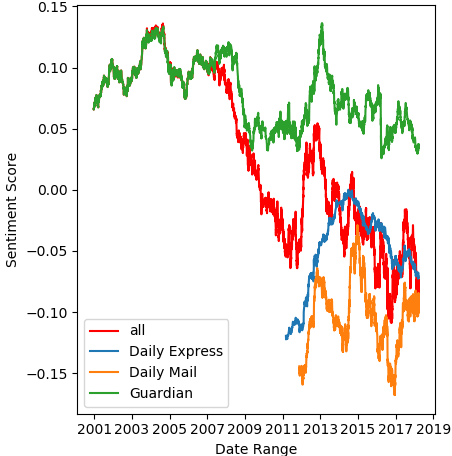
\includegraphics[width=0.5\textwidth]{vader.png}
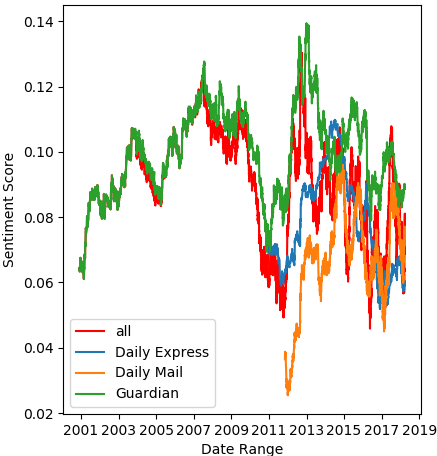
\includegraphics[width=0.5\textwidth]{openai.png}
(Left = VADER, Right = OpenAI's model)
\vspace{0.5em}

These plots show that the version implementing VADER is more consistent in distinguishing between different sources, with a smoother trend line; while the line produced by the version implementing OpenAI's model has higher randomness; despite using the same moving average window size (500 articles) in both plots.

% discuss about how VADER, although much simpler than other models, is more generalisable than stat-ML/NN models trained on different domains ("These results came as a surprise as...")
These results came as a surprise, due to the simplicity of VADER's rule-based model, relative to other implemented models (refer to section \ref{tc-sentiment} or \ref{des-sentiment-comparison} for a list and short description of these sentiment scorer implementations) based on supervised machine learning or neural network approaches.
The suspected reason behind this is that because these supervised machine learning and neural network models were trained on data from other domains (mainly tweets, movie reviews, or Amazon reviews), and the parameters learned by the model does not necessarily translate well to this domain (sentences from news articles referring to disabilities or people with disabilities). 
Meanwhile, VADER's simpler rule-based model is more generalisable, as it simply checks for a set of rules to determine general positive/negative text (instead of using parameters learned from training data).

It is likely that a supervised machine learning or neural network model, trained on an adequately large labelled dataset (likely at least tens or hundreds of thousands of sentences) from this domain, could strongly out-perform VADER, given that the accuracy of sentiment scores from OpenAI's implementation (based on a neural network model) was very close to VADER's, despite the model being trained on a different domain (82 million Amazon product reviews). 
However, such a large labelled dataset was infeasible for the scope of this experiment.

% Mention how only results from VADER will be considered relevant from this point
For the following sections, all sentiment score results mentioned are those scored by VADER's implementation \cite{VADER}.
Additionally, news articles with a VADER sentiment score of 0.0 were excluded from the plotted dataset, as they are presumed to be non-opinionated and thus irrelevant in sentiment measurement.

\section{Sentiment Score: Plots and Trends} \label{Sentiment score: plots and trends}
% graphs, tables (mean std dev) relating to sentiment
For the `disabled' topic, the VADER sentiment scores of all articles within the dataset (16,411 articles in total within the topic) were plotted with regards to their publication date and source of article (Daily Express, Daily Mail, Guardian) in several visual representations (as defined in section \ref{des-visualisation}).

\begin{center}
	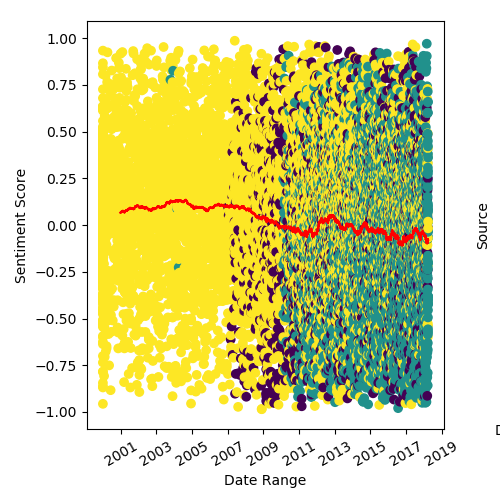
\includegraphics[height=0.5\linewidth]{row-1-col-1.png}
\end{center}

The first plot is a scatter plot of publication date (X) vs sentiment scores (Y), coloured based on publication source (Z). 
Due to the large dataset size, the scatter plot does not provide much information with regards to distributions and trends, although it shows how the Daily Express (blue-green) only retains articles from after \textapprox2007, the Daily Mail (dark blue) only retains articles from after \textapprox2010, and the Guardian (yellow) only retains articles from after \textapprox2000, as mentioned in section \ref{limitations}.
A moving average line (with a window size of 500) of sentiment scores over time of all articles (regardless of source) is drawn over the scatter plot.

\begin{center}
	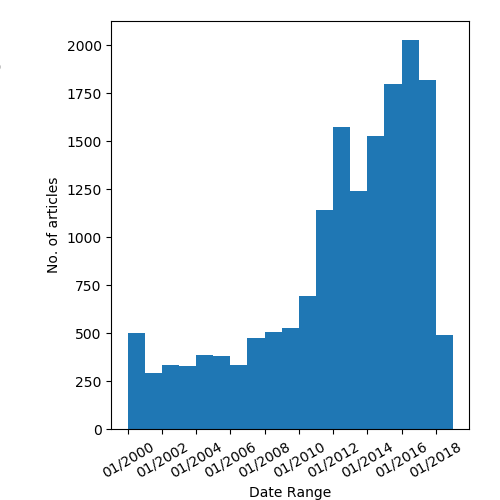
\includegraphics[width=0.5\linewidth]{row-1-col-3.png}
\end{center}

A histogram of the number of articles in each year was plotted to show the distribution of articles over time in the dataset. 
This do not necessarily reflect how many articles was published regarding the topic for every year, as news publishers often do not retain all historical articles and the amount of retained articles tend to be higher in more recent years, and vice versa.
That said, a spike in the number of articles in the dataset was visible in 2012, which correspond to increased media coverage of disabilities and people with disabilities around the 2012 London Paralympics.

\begin{center}
	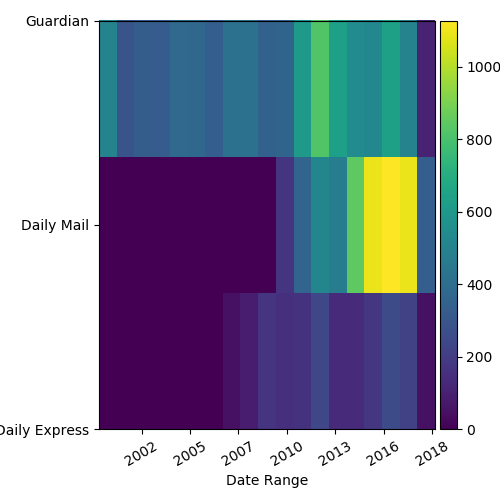
\includegraphics[width=0.5\linewidth]{row-1-col-2.png}
\end{center}
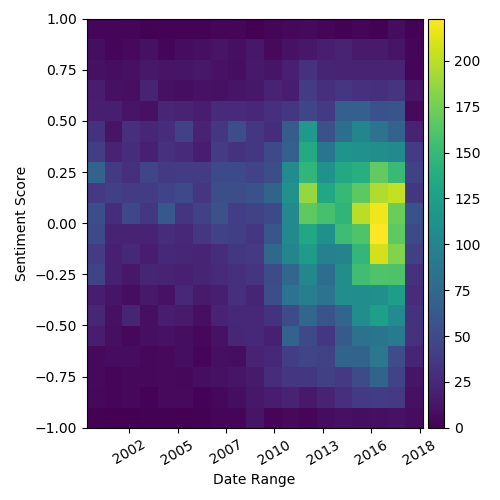
\includegraphics[width=0.5\linewidth]{row-2-col-1.png}
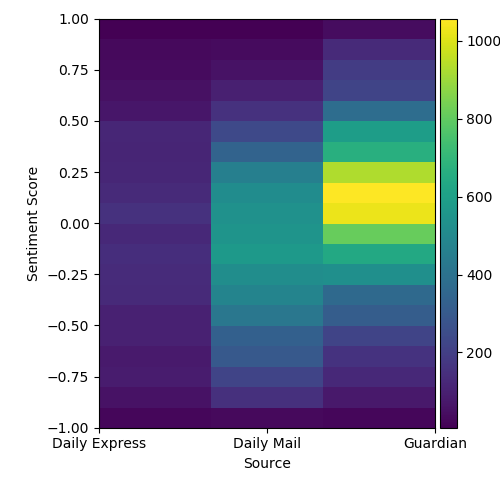
\includegraphics[width=0.5\linewidth]{row-2-col-2.png}

Three two-dimensional histograms that show the distribution of articles for:
\begin{itemize}
	\item The number of news articles for each year (X) and source (Y) in the dataset.
	\item The distribution of sentiment scores (Y) for each year (X).
	\item The distribution of sentiment scores (Y) for each source (X).
\end{itemize}
were plotted. 
The year-source plot show that the dataset consist almost entirely of Guardian articles for the years 2000--2006. In 2007 Daily Express articles and in 2010 Daily Mail articles starts to appear, although Guardian articles still predominate between 2007--2013, until in 2014 where Daily Mail articles start to outnumber Guardian articles by roughly 2:1.

The year-sentiment plot show that the sentiment distribution of most news articles lie somewhere between 0.0 and 0.3 from 2000--2009, and between -0.3 and 0.3 (but with more variance/outliers) from 2010--2018. 
It also showed a slight `drop' in the sentiment distribution (or an increase of news articles with negative sentiment scores) around 2016.

The source-sentiment plot show (roughly) that the Guardian has a higher mean and less variance than the Daily Mail, and the Daily Express is barely visible due to the lower sample size of Daily Express articles in the dataset.
However, the uneven sample size (i.e. more Guardian articles vs Daily Mail or Daily Express articles over the full dataset) makes this visual representation hard to compare. The violin \cite{hintze1998violin} and box-and-whiskers plot \cite{tukey1977exploratory} show a better representation of this source-sentiment data:

\begin{center}
	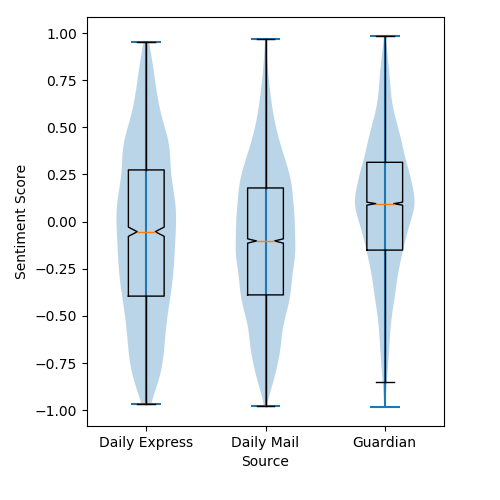
\includegraphics[width=0.5\linewidth]{row-3-col-1.png}
\end{center}

The violin and box-and-whiskers plot show that the Guardian's mean sentiment score (0.074) is higher than the Daily Mail's (-0.104) or the Daily Express's (-0.060).
Furthermore, the violin plot component show that the Guardian's distribution is more `compact' around the mean (std. dev. = 0.363), the Mail has a slightly higher variance (std. dev. = 0.386), and the Express has the highest variance (std. dev. = 0.447). A version that shows violin plots for each 2-year period were also plotted (green = Guardian, blue = Daily Express, orange = Daily Mail):

\begin{center}
	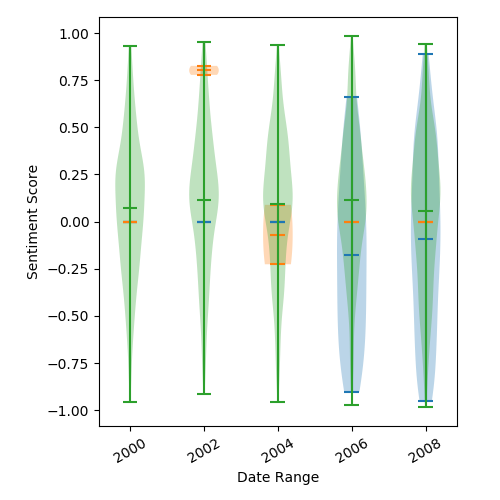
\includegraphics[width=0.4\linewidth]{row-3-col-2.png}
	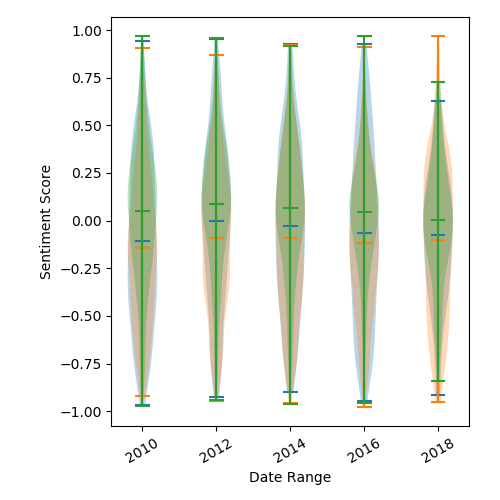
\includegraphics[width=0.4\linewidth]{row-3-col-3.png}

	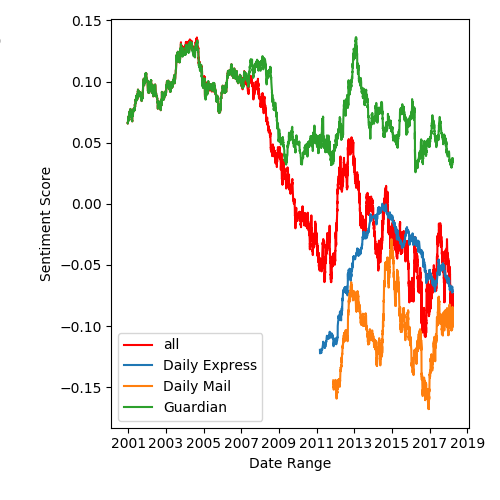
\includegraphics[width=0.5\linewidth]{row-2-col-3.png}
\end{center}

From the year-sentiment plot showed that there is an apparent trend of declining sentiment scores over time. 
However, the moving average line plot (where each data point shows the mean sentiment score of 500 consecutive articles, and the last article's date) show that this is not necessarily the case. 
When only taking into account articles from the same source, the moving average sentiment score stays roughly consistent.
However, the decreasing trend in `all' is likely better attributed to the (gradually) decreasing proportion of Guardian articles and the (gradually) increasing proportion of Daily Mail articles in the dataset.

For topics other than `disabled', the majority show a similar constant trend for articles within the same source, although this is not always the case. The topic `autism', for instance, show a positive trend in sentiment scores year-on-year:

\begin{center}
	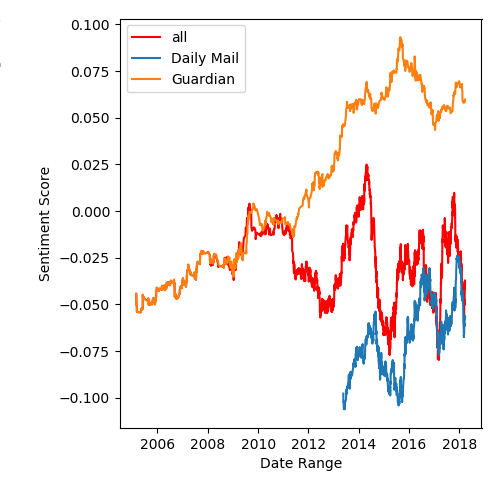
\includegraphics[width=0.5\linewidth]{autism.png}
\end{center}

Note also that the Daily Express is not plotted for this topic, due to the sample size being too small (128 articles), lower than the moving average window (316 articles on this topic); a common occurrence for most other topics (as defined in \ref{topics}).

\section{Sentiment Score: Statistical Comparison of Sources} \label{Sentiment score: statistical comparison of different sources}

% Mann-Whitney U analysis (re-define it again, what it means for statistical significance etc)
To test whether the differences between the distributions of each source are statistically significant, the Mann-Whitney $U$ Test \cite{mann1947test} was invoked.
The Mann-Whitney $U$ Test is a mathematical function that tests the null hypothesis that given a randomly-selected value from a distribution, and a second randomly-selected value from a second distribution, the first value is equally likely to be less than or greater than the second value.
If the null hypothesis holds true, then there is no statistically significant difference between the two distributions.
The Mann-Whitney $U$ Test function returns a $p$-value score, which is a measure of the probability that the null hypothesis is correct.
In this experiment, two distributions are considered significantly different if the $p$-value returned by the Mann-Whitney $U$ Test is lower than 0.05.

% Table of Mann-Whitney U scores for each topic and source comparisons, overlap with n_articles for each source
Below is a table of $p$-values from Mann-Whitney $U$ Test results for every source combination in the dataset, for every topic (including topics other than `disabled'):

\noindent
\begin{tabu} to \textwidth { | X[c] | X[c] | X[c] | X[c] | }
	\hline
	Topic & Guardian \textgreater\space Daily Mail & Guardian \textgreater\space Daily Express & Daily Express \textgreater\space Daily Mail  \\
		\hline
	Disabled & \textbf{2.66 * 10\textsuperscript{-167}} & \textbf{2.29 * 10\textsuperscript{-35}} & \textbf{0.000108}  \\
	\hline
	Autism & \textbf{3.00 * 10\textsuperscript{-12}} & 0.137 & 0.184  \\
	\hline
	Blind & 0.335 ** & \textbf{1.62 * 10\textsuperscript{-9}} & \textbf{6.57 * 10\textsuperscript{-9} **} \\
	\hline
	Cerebral Palsy & 0.469 & 0.156 ** & 0.169  \\
	\hline
	Deaf & \textbf{6.30 * 10\textsuperscript{-10}} & 0.141 & 0.0833  \\
	\hline
	Developmental Delay & 0.383 & \textbf{0.00179} & \textbf{0.00326 **}  \\
	\hline
	Dyslexia & 0.0740 & 0.362 & 0.464 **  \\
	\hline
	Epilepsy & \textbf{3.39 * 10\textsuperscript{-5}} & 0.0579 & 0.322 **  \\
	\hline
	Mental Illness & \textbf{3.54 * 10\textsuperscript{-76}} & \textbf{1.51 * 10\textsuperscript{-9}} & 0.102 **  \\
	\hline
	Mute & \textbf{6.78 * 10\textsuperscript{-5}} & \textbf{0.0311} & 0.346 ** \\
	\hline
	Paralysis & \textbf{2.73 * 10\textsuperscript{-5}} & \textbf{0.00909} & 0.0827 **  \\
	\hline
	Speech Impairment & 0.235 & \textbf{0.0200} & 0.0546 **  \\
	\hline
\end{tabu}
** Indicates where the reverse assumption is true (e.g. Daily Mail \textgreater\space Daily Express instead of Daily Express \textgreater\space Daily Mail)

This data shows that a statistically-significant distinction can be proven between the sentiment score distributions of two sources for 17 / 36 of cases.
(Cases where there exists a distinction between the two distributions are highlighted in bold)
In particular, Guardian \textgreater\space Daily Mail is true for 7 / 12 cases, Guardian \textgreater\space Daily Express is true for 7 / 12 cases, Daily Express \textgreater\space Daily Mail is true for 1 / 12 cases, and Daily Mail \textgreater\space Daily Express is true for 2 / 12 cases.
Comparing these values to the size of each dataset (section \ref{dataset-size}), Lower $p$-values tends to correlate well with larger sample sizes (i.e. the higher the sample size of both distributions, the higher the chance that there exist a statistically-significant difference).

% do year on year analysis on disabled topic
For the `disabled' topic, the Mann-Whitney $U$ Test was also performed to compare between Daily Mail, Daily Express, and The Guardian for each year's subset between 2007 and 2018 (Before 2007, there were not enough non-Guardian articles in the dataset to make a comparison).
The $p$-values of these comparisons are shown below:

\noindent
\begin{tabu} to \textwidth { | X[c] | X[c] | X[c] | X[c] | }
	\hline
	Topic & Guardian \textgreater\space Daily Mail & Guardian \textgreater\space Daily Express & Daily Express \textgreater\space Daily Mail  \\
	\hline
	2007 & N/A & \textbf{5.24 * 10\textsuperscript{-6}} & N/A  \\
	\hline
	2008 & N/A & 0.0739 & N/A  \\
	\hline
	2009 & N/A & \textbf{2.24 * 10\textsuperscript{-5}} & N/A  \\
	\hline
	2010 & \textbf{6.00 * 10\textsuperscript{-7}} & \textbf{6.89 * 10\textsuperscript{-6}} & 0.360 **  \\
	\hline
	2011 & \textbf{5.73 * 10\textsuperscript{-16}} & \textbf{9.73 * 10\textsuperscript{-5}} & \textbf{0.0355}  \\
	\hline
	2012 & \textbf{4.44 * 10\textsuperscript{-17}} & \textbf{0.00371} & \textbf{0.000739}  \\
	\hline
	2013 & \textbf{5.03 * 10\textsuperscript{-16}} & \textbf{0.00351} & 0.0827  \\
	\hline
	2014 & \textbf{1.27 * 10\textsuperscript{-9}} & \textbf{0.00208} & 0.321  \\
	\hline
	2015 & \textbf{6.87 * 10\textsuperscript{-17}} & \textbf{0.00855} & \textbf{0.00718}  \\
	\hline
	2016 & \textbf{4.63 * 10\textsuperscript{-26}} & \textbf{4.74 * 10\textsuperscript{-6}} & 0.0576  \\
	\hline
	2017 & \textbf{3.39 * 10\textsuperscript{-13}} & \textbf{0.00244} & 0.0867  \\
	\hline
	2018* & 0.122 & 0.120 & 0.328  \\
	\hline
\end{tabu}

* 2018 data is incomplete and would only include articles up to (approximately) end of March.

** Indicates where the reverse assumption is true (e.g. Daily Mail \textgreater\space Daily Express instead of Daily Express \textgreater\space Daily Mail)

\section{Key Terms: Plots and Trends} \label{Key terms: plots and trends}

Apart from sentiment score analyses, NLP approaches can also be applied to extract various other syntax-based features and analyse trends based on them.
Features based on counting words (term frequency) are a mainstay of NLP research.
Besides sentiment scores, the pipeline also extracts the term frequency of all terms that matches a key term's lemma, from all news articles (refer to section \ref{des-matching} for details).
This information is used to plot trends on key term usage over time.

A weak custom stemmer, that only stems plural and past/future tense forms, but not other suffixes, was used to group equivalent terms together regardless of context, without losing additional meaning from affixes.
For example, `illness' and `illnesses' are equivalent, but `ill' and `illness' are still considered distinct.
Terms were also converted to lower case such that capitalisation was ignored, thus e.g. `Disability' and `disability' are equivalent.

For each term, a measure of average term occurrence, which measures the expected number of occurrences of a term in an article for a given year, is computed for each year between 2000 and 2018.
Refer to section \ref{des-visualisation} for a formal definition of this metric.

With this approach, we measured the year-on-year average term occurrence trends of each key term in the `disabled' topic, and plotted the results in line graphs (one for each key term):

\noindent
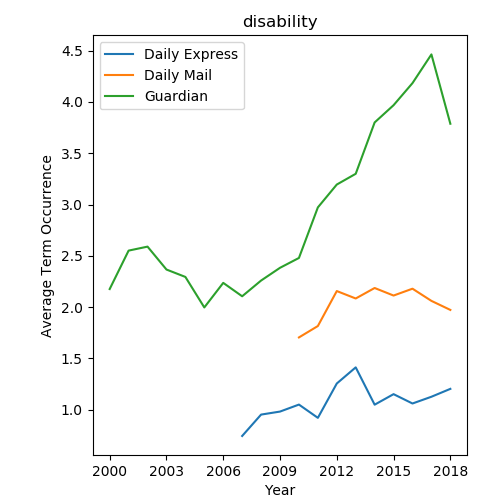
\includegraphics[width=0.5\linewidth]{terms1.png}
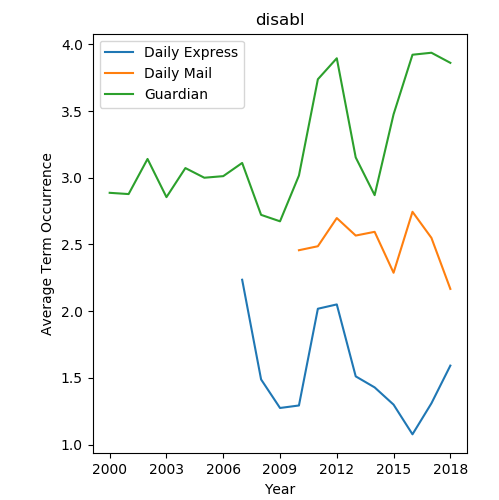
\includegraphics[width=0.5\linewidth]{terms2.png}

\noindent
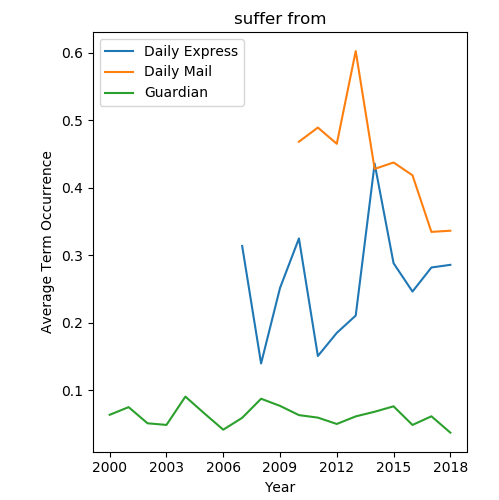
\includegraphics[width=0.5\linewidth]{terms3.png}
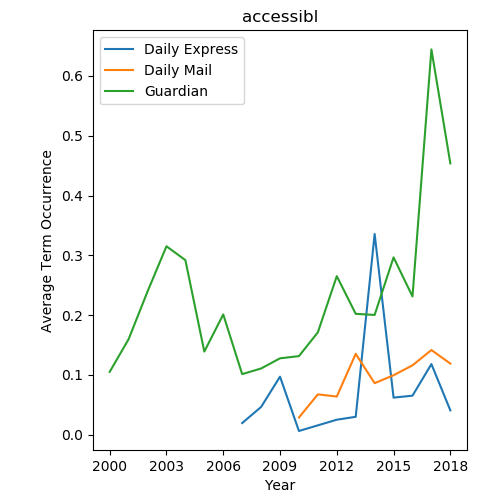
\includegraphics[width=0.5\linewidth]{terms4.png}

\noindent
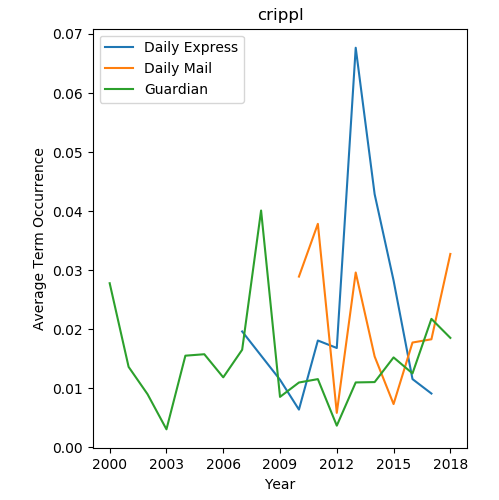
\includegraphics[width=0.5\linewidth]{terms5.png}
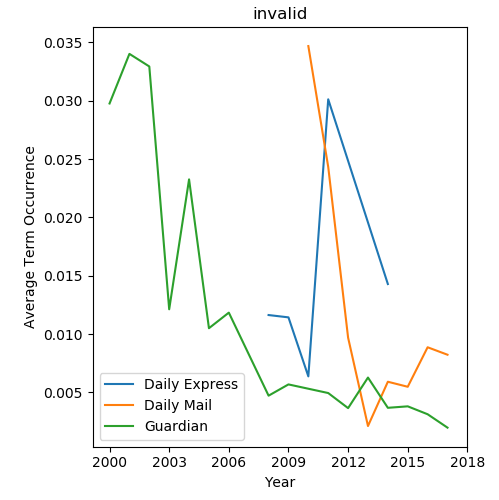
\includegraphics[width=0.5\linewidth]{terms6.png}

\noindent
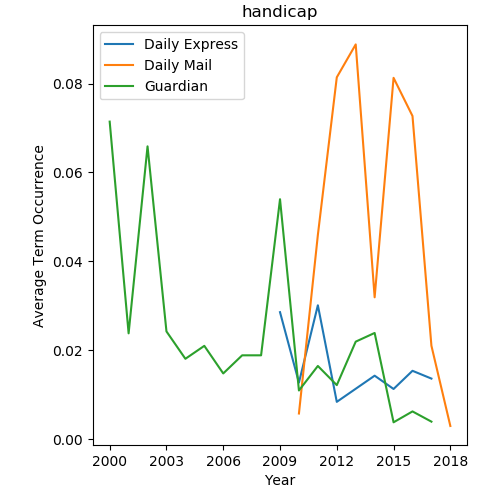
\includegraphics[width=0.5\linewidth]{terms7.png}
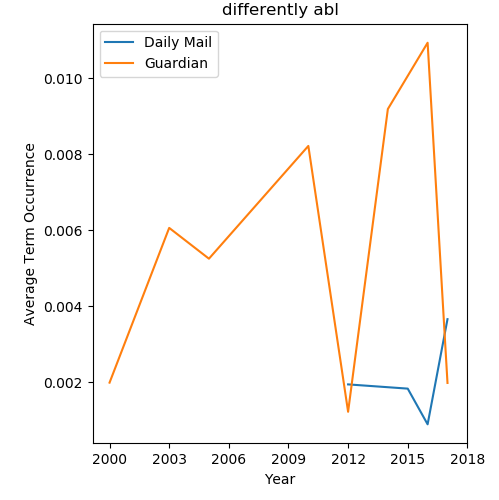
\includegraphics[width=0.5\linewidth]{terms8.png}

\begin{center}
	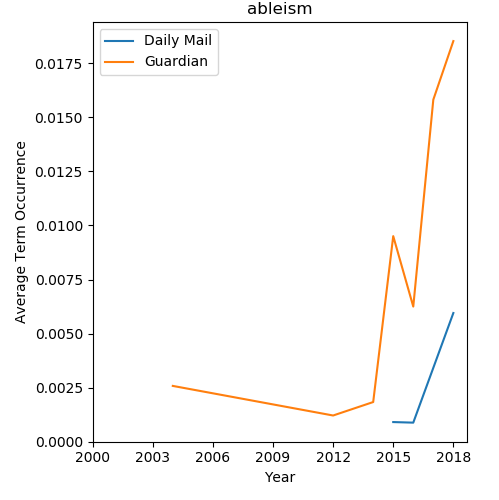
\includegraphics[width=0.5\linewidth]{terms9.png}
\end{center}

% key terms analysis: most of them stay constant over the period (probably because 18 years data is quite short for cultural shifts), but mention the few where visible trends can be seen + show graphs. Also smaller sample sizes.
These line plots show that, for most key terms, the average term occurrence trends mostly stay constant year-on-year for the same publisher.
While this exact approach was successfully used to detect cultural changes in British media \cite{lansdall2017content}, in this case the sampled time period is much shorter for significant linguistic changes to have occurred (18 vs 150 years).

In this case, increasing/decreasing year-on-year trends are only visible for a select few terms.
The usage of the terms `invalid' and `handicap(ped)', for example, show a rapidly decreasing trend between 2000 and 2018 on the Guardian.
`accessible', on the other hand, show an increasing trend on the Guardian.
While the data is less consistent for the Daily Express and Daily Mail, this was likely caused by a lack of data for these sources before 2007 and 2010 respectively, and a smaller overall sample size (especially for the Daily Express).

% also mention source-by-source variations
These plots also show variations in term usage between different publishers.
For example, the Guardian refers to `disability' or `disabl(ed)' by name consistently more often than the Daily Mail or Daily Express, and uses the terms `suffers(s) from' consistently less often.

%% Describe your testing strategy (unit, functional, acceptance testing; and how they are carried out). How were test cases selected?
% Not Applicable

%% Examples of specific tests and how they were carried out (e.g., using mock objects to break dependencies). Focus on the interesting cases.
% Not Applicable

%% A summary of the test results and what coverage was achieved. Detailed test reports should appear in the appendix, if they add useful information or you want to demonstrate the kinds of tests and coverage achieved.
% Not Applicable

%% If your project requires substantial evaluation of data and results, evaluation of algorithms, or other forms of testing that are not code-based, then adapt this chapter to suit.
%% This chapter will typically be 2-4 pages in length but could be more depending on the depth of testing done. If you need to do a detailed evaluation for a more mathematical or theory-based project, then this chapter could well be more substantial.


\chapter{Conclusions} \label{Conclusions}  % 2-4 pages
%% Wrap-up and final thoughts on your project. 
%% This chapter is typically 2-4 pages long but could be longer if the project work requires more extensive evaluation.

% do not write text here

\section{Achievements} \label{Achievements}
%% Summarise the achievements to confirm the project goals have been met.
%% A summary of what the project has achieved. Make sure that you address each goal set out in the Introduction chapter, to show that you have achieved what you claimed you would. Don’t leave any loose ends

The aim of this project was to explore the feasibility of exploiting NLP technologies to discover trends with regards to specific topics, with regards to the representation of disabilities and people with disabilities in British online news media.
The results to this experiment showed that this is feasible.
By analysing a dataset of 16,411 news articles related to the key terms `disabled', `disability', `handicapped', `cripple', `invalid', `accessible', `ablism', and `ableism'; the results in section \ref{Sentiment score: plots and trends} plotted trends in the variation of modelled sentiment scores across three different news publishers (Daily Express, Daily Mail, and Guardian) and over time.
The results of Mann-Whitney $U$ statistical test in section \ref{Sentiment score: statistical comparison of different sources} showed that the differences in sentiment score distributions between the three publishers are statistically significant for the `disabled' topic, and showed that `Guardian \textgreater\space Daily Mail' and `Guardian \textgreater\space Daily Express' is true for every year between 2010 and 2017.
Furthermore, the results of analysing average term occurrences of key terms, as shown in section \ref{Key terms: plots and trends}, identified increasing or decreasing trends for the terms `invalid', `handicap(ped)', and `accessibl(e)' for the Guardian; and showed variations in term usage/popularity between different publishers.

This experiment was repeated across 11 other topics (as defined in section \ref{topics}), with varying degrees of success. 
The lower sample size of news articles related to other topics in the dataset, and decreased effectiveness of the filter with regards to the selection of topics with more ambiguous keywords (e.g. `blind', `mute', `paralysed', and `stutter'), were major factors in the variability of results.
The full results of the experiment for all 12 topics are available in the Appendix.
 
The experiment also showed that it was feasible to collect and analyse a large dataset of 305,185 news articles, reduced to 48,967 articles after filtering, within a reasonable time frame using consumer-grade hardware (Intel i7-6700HQ CPU @ 2.60GHz, NVIDIA GeForce GTX 1060 GPU, 200 Mbit/s download speed).
Additionally, the vast majority of the time was spent on data collection from online sources, and an analysis of existing news articles corpora would take less time (approximately 0.37 seconds per article in extracting text features, with negligible sentiment scoring runtime using VADER).
With more powerful hardware available to institutions and large corporations, this approach should scale well to analyse corpora consisting of millions of news articles in reasonable time.

\section{Evaluation} \label{Evaluation}
%% Evaluation of the work (this may be in a separate chapter if there is substantial evaluation).
%% A critical evaluation of the results of the project (e.g., how well were the goals met, is the application fit for purpose, has good design and implementation practice been followed, was the right implementation technology chosen and so on).

This experiment showed that it was feasible to apply existing open-source NLP technologies to discover trends on a large dataset of news articles in this domain, which achieved the primary aim of this project.
The solution developed to perform this experiment delivered in performing data collection and filtering of a dataset of 305,185 news articles; and feature extraction (collecting relevant sentences and key term frequencies), sentiment scoring, statistical analysis, and data visualisation of 48,967 news articles after filtering.
The modular approach to solution design, with five separate components for each sub-task (data collection, filtering, feature extraction, sentiment scoring, and data analysis/visualisation), was ideal in this research, enabling experimentation in various components (e.g. trying multiple sentiment scorer implementations and data visualisation plots) without having to change or re-run code for other components.
This solution achieved the project's goals sufficiently as a proof of concept, and delivered meaningful results.

% Choice of technologies (what's good e.g. Python, range of libraries, plotting, etc.; what can be improved i.e. try other methods e.g. topic models for filtering, inconsistency of models used e.g. stemming with NLTK for filtering vs lemmatising with SpaCy for rule-based sentence matching)
The choice of NLP techniques and technologies, extracted features, statistical metrics, and visualisation tools are sufficient, and achieved results, but leaves room for further improvement.
The main limitation in this research was a lack of labelled data for both filtering on-topic/off-topic articles and sentiment scoring, which led to inconsistencies in both aspects.
In particular, the filter had issues with ambiguous terms such as `blind', `mute', `paralysed', and `stutter'; a supervised filter may be able to overcome this issue by taking the word's context in the sentence into account (for example, by also evaluating other words in the sentence), and also provide better evaluation of filter accuracy. 
Given this constraint, the filter worked adequately well to prepare the dataset for the experiment, and limited sampling of on-topic/off-topic articles showed that the approach was sufficiently accurate for the majority of topics.

Without labelled data for sentiment scoring, the only possible options were to use generalised supervised models trained on other domains, or to use a less complex model based on rule matching.
It was found that a less complex model based on rule matching (VADER \cite{VADER}) outperformed advanced supervised models based on statistical classifiers or neural networks trained on different domains.
However, VADER is still highly inconsistent in this domain (with an accuracy of 0.789), and although it was sufficient to discover trends in this experiment, it is likely that domain-specific supervised model would outperform it.
With a more consistent sentiment scorer, it is likely that the variance of sentiment scores within subsets would be lower, and the trend lines generated in data visualisation would be more consistent.

The usage of different NLP libraries in separate components, such as NLTK's stemmer for filtering and SpaCy's lemmatiser for feature extraction, also left occasional inconsistencies, such as rare cases of the feature extractor not finding any relevant sentences in articles the filter deemed on-topic.

\section{Future Work} \label{Future Work}
%% How the project might be continued, but don't give the impression you ran out of time!
%% Future work. How could the project be developed if you had another 6 months. Take care to differentiate between what you have done to satisfy your stated project goals, and work that could be done to meet extended goals.

% Implications of NLP for future media studies, call for similar analyses to be conducted in other domains (mention additional information that can be discovered by using computational NLP and processing a much larger sample of text) 
The results showed that this computational NLP-based approach is effective in analysing news media with regards to the media representation of disabilities and people with disabilities.
This could have a substantial impact on how research will be conducted for similar studies.
Past studies (such as \cite{gold1999media, coverdale2002depictions, jones2009representations, devotta2013representations}) could be revisited using computational approaches to analyse a much larger sample size of articles, to improve the certainty and representativeness of the conclusion and possibly identify trends by varying for independent variables such as the publisher and date published.

% Purpose built sentiment model trained to a a labelled sample: in this analysis vader performed best although it's a very simple model as other, more complex pre-trained models were trained on other domains and is less generalisable. However, OpenAI's model came very close despite this, and a similar approach using deep learning or statistical ML models, trained on a labelled sample of positive/negative/neutral sentences in this domain, would have much improved sentiment score reliability (and thus quality of analyses)
As mentioned above, the lack of labelled domain-specific dataset (of sentences from news articles relating to disabilities, labelled with `positive' or `negative') for sentiment scoring limited the sentiment scores' accuracy in this experiment.
While exploring general-purpose open-source sentiment scorer implementations, it was found that a simple rule-based model outperformed the more sophisticated statistical classification or neural network models for the sentiment scoring task, as they were trained with labelled dataset from other domains.
However, one of the neural network based models (OpenAI \cite{OpenAI}) came close to the selected model (VADER \cite{VADER}), despite being trained on a completely separate domain (Amazon reviews), which suggest that a domain-specific supervised model would strongly out-perform VADER given sufficient, high-quality training data.
Thus, if an adequately large dataset of labelled sentences (likely \textgreater10,000 sentences would be required) for this domain could be compiled, future work could use this dataset to train a supervised model to improve the accuracy of the sentiment scorer.
With a more accurate and more consistent sentiment scorer, it is likely that the variance of sentiment scorers within subsets would be lower, and it would be possible to derive clearer trends and obtain statistically-significant comparisons on subsets with lower sample sizes (e.g. smaller time intervals).

Similarly, a supervised filter, trained on a labelled dataset of on-topic/off-topic news articles, would improve filtering accuracy and reduce off-topic articles in the filtered dataset, especially for trickier topics with ambiguous terms such as `blind' or `mute'.

% Expand sources - Develop API where others can use and adapt the code, change topics / keywords / key phrases / query terms, add/change sources by developing their own scrapers (with an interface for the scraper), document code and improve code readability and output file structure, output sample on-topic/off-topic articles to help them set rank threshold, maybe even an API to provide their own sentiment model(s) as parameter given an interface
Another potential application is to develop a public interface that allow users to retrieve the results of analyses performed in this experiment for other domains, given a list of topics (key terms and query terms) and/or an existing text corpora provided by the user.
The solution described in this project would have to be generalised with an interface, where users can provide their own scrapers that implement a well-documented set of functions for other news websites/sources, define their own list of topics, key terms, and query terms, and possibly even change the independent variables and subset intervals for the analysis.
It would also need to provide clear documentation on its usage and expected input structure/format.
Such a solution would provide researchers with the tools to perform similar research with ease, and possibly build on the tool as part of other projects using it as a component.

\appendix
\addtocontents{toc}{\protect\setcounter{tocdepth}{0}}  % don't show appendix sections in ToC

\printbibliography[heading=bibintoc]

\chapter{Appendix: All results}  % appendix A

\newpage
\section{Topic: `disabled'}
Key Terms: `disabled', `disability', `handicapped', `cripple', `invalid', `accessible', `ablism', `ableism', `differently abled'

\noindent Query Terms: `disabled', `disability', `ablism', `ableism', `differently abled'

\noindent Sample size, n = 16,411

\subsection{Sentiment Score Plots}
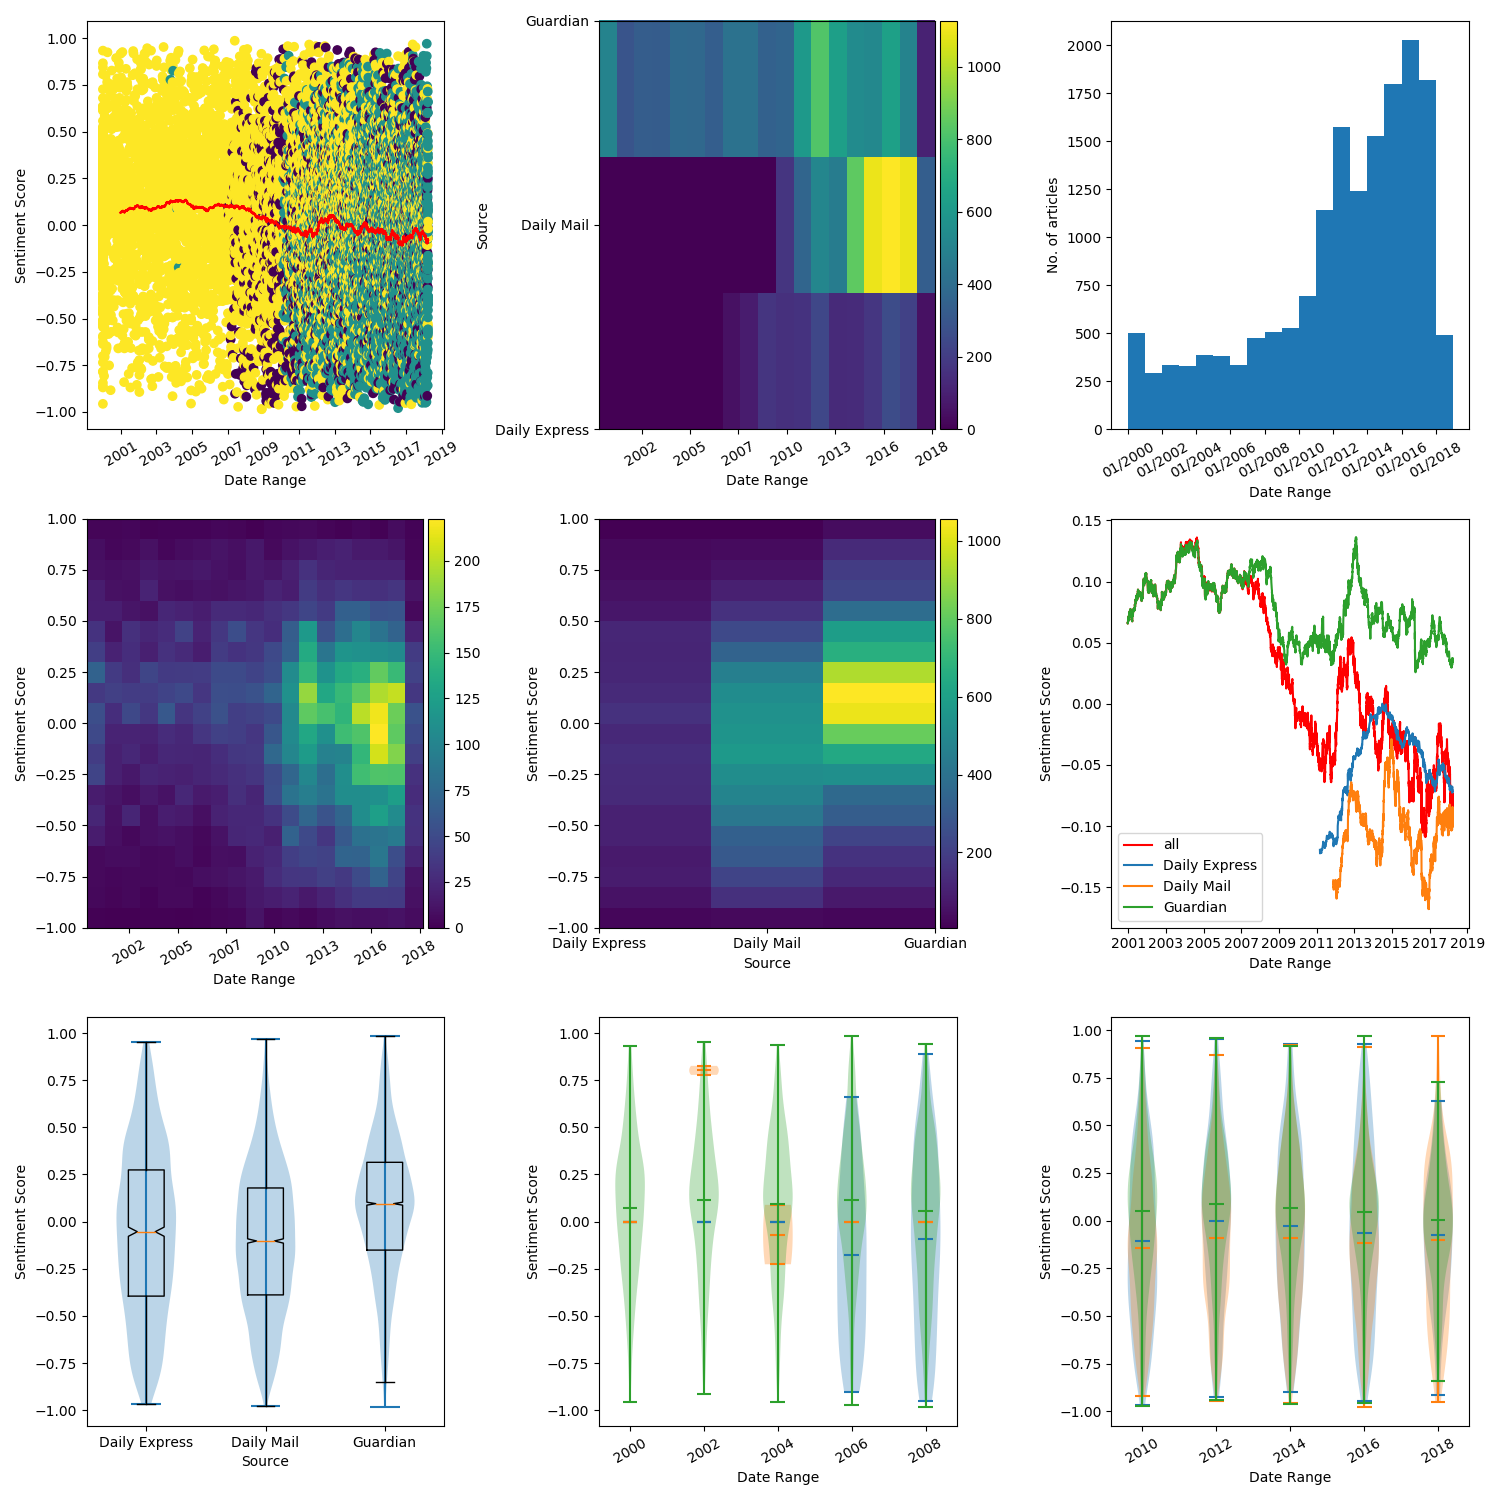
\includegraphics[width=\textwidth]{raw/disabled.png}

\subsection{Mann-Whitney $U$ Test Results ($p$-values)}
\noindent
\begin{tabu} to \textwidth { | X[c] | X[c] | X[c] | X[c] | }
	\hline
	Topic & Guardian \textgreater\space Daily Mail & Guardian \textgreater\space Daily Express & Daily Express \textgreater\space Daily Mail  \\
	\hline
	All & 2.66 * 10\textsuperscript{-167} & 2.29 * 10\textsuperscript{-35} & 0.000108  \\
	\hline
	2007 & N/A & 5.24 * 10\textsuperscript{-6} & N/A  \\
	\hline
	2008 & N/A & 0.0739 & N/A  \\
	\hline
	2009 & N/A & 2.24 * 10\textsuperscript{-5} & N/A  \\
	\hline
	2010 & 6.00 * 10\textsuperscript{-7} & 6.89 * 10\textsuperscript{-6} & 0.360 **  \\
	\hline
	2011 & 5.73 * 10\textsuperscript{-16} & 9.73 * 10\textsuperscript{-5} & 0.0355  \\
	\hline
	2012 & 4.44 * 10\textsuperscript{-17} & 0.00371 & 0.000739  \\
	\hline
	2013 & 5.03 * 10\textsuperscript{-16} & 0.00351 & 0.0827  \\
	\hline
	2014 & 1.27 * 10\textsuperscript{-9} & 0.00208 & 0.321  \\
	\hline
	2015 & 6.87 * 10\textsuperscript{-17} & 0.00855 & 0.00718  \\
	\hline
	2016 & 4.63 * 10\textsuperscript{-26} & 4.74 * 10\textsuperscript{-6} & 0.0576  \\
	\hline
	2017 & 3.39 * 10\textsuperscript{-13} & 0.00244 & 0.0867  \\
	\hline
	2018* & 0.122 & 0.120 & 0.328  \\
	\hline
\end{tabu}

\noindent * 2018 data is incomplete and would only include articles up to (approximately) end of March.

\noindent ** Indicates where the reverse assumption is true (e.g. Daily Mail \textgreater\space Daily Express instead of Daily Express \textgreater\space Daily Mail)

\subsection{Key Term Trend Plots}
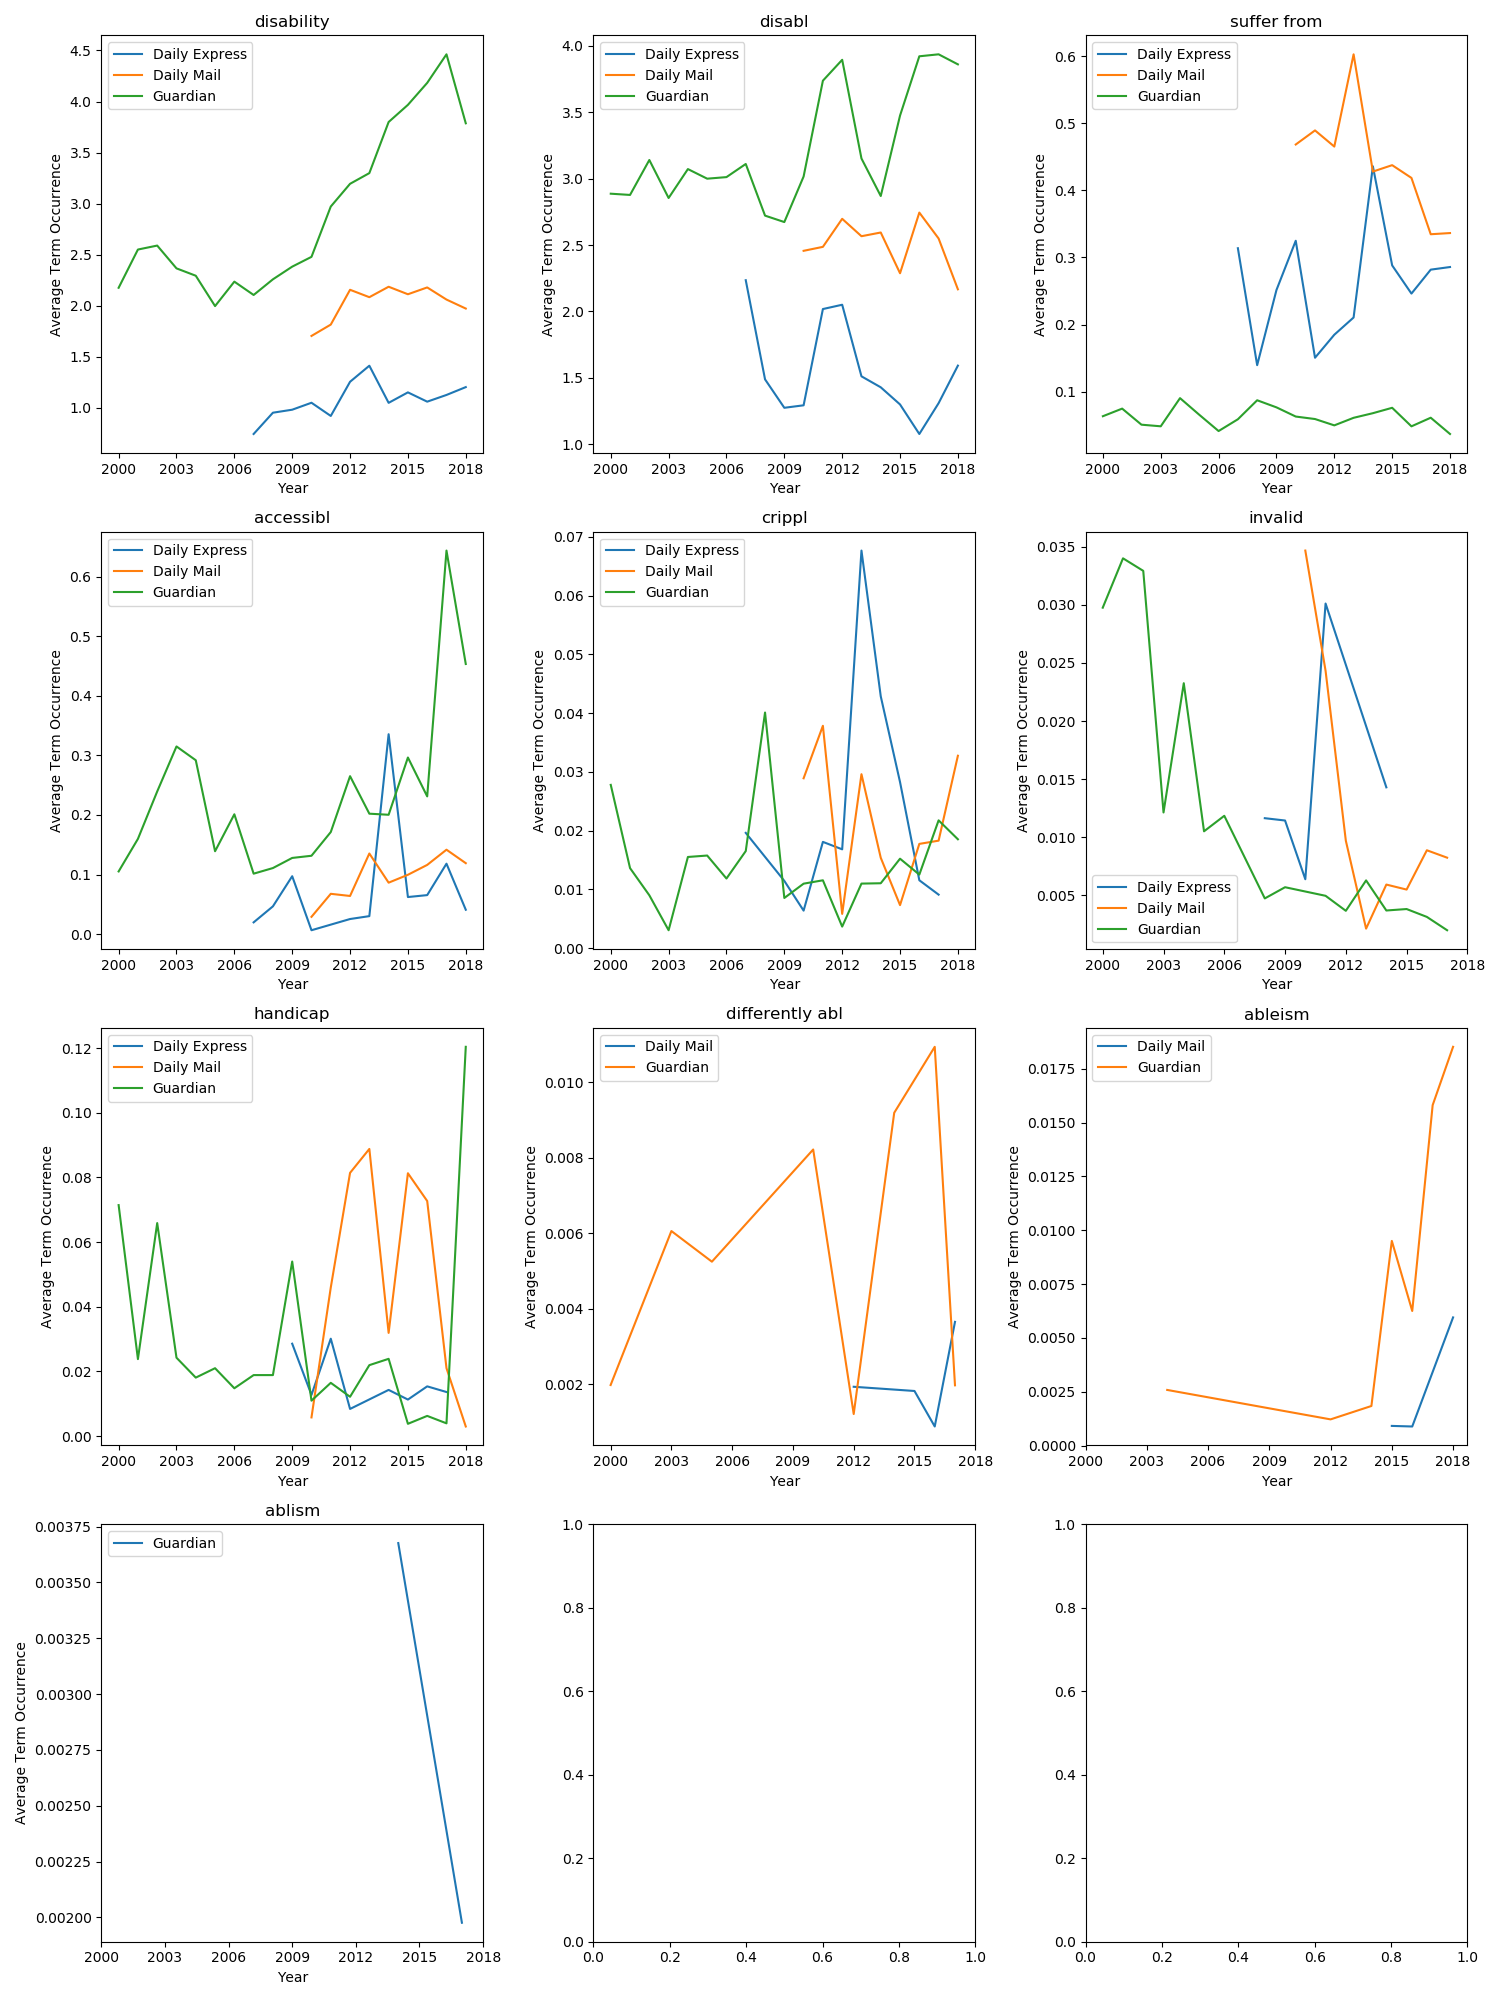
\includegraphics[width=\textwidth]{raw/disabled-terms.png}

\newpage
\section{Topic: `autism'}
Key Terms: `autism', `autistic', `asperger\textbackslash's', `ASD'

\noindent Query Terms: `autism', `autistic', `asperger\textbackslash's', `ASD'

\noindent Sample size, n = 3,161

\subsection{Sentiment Score Plots}
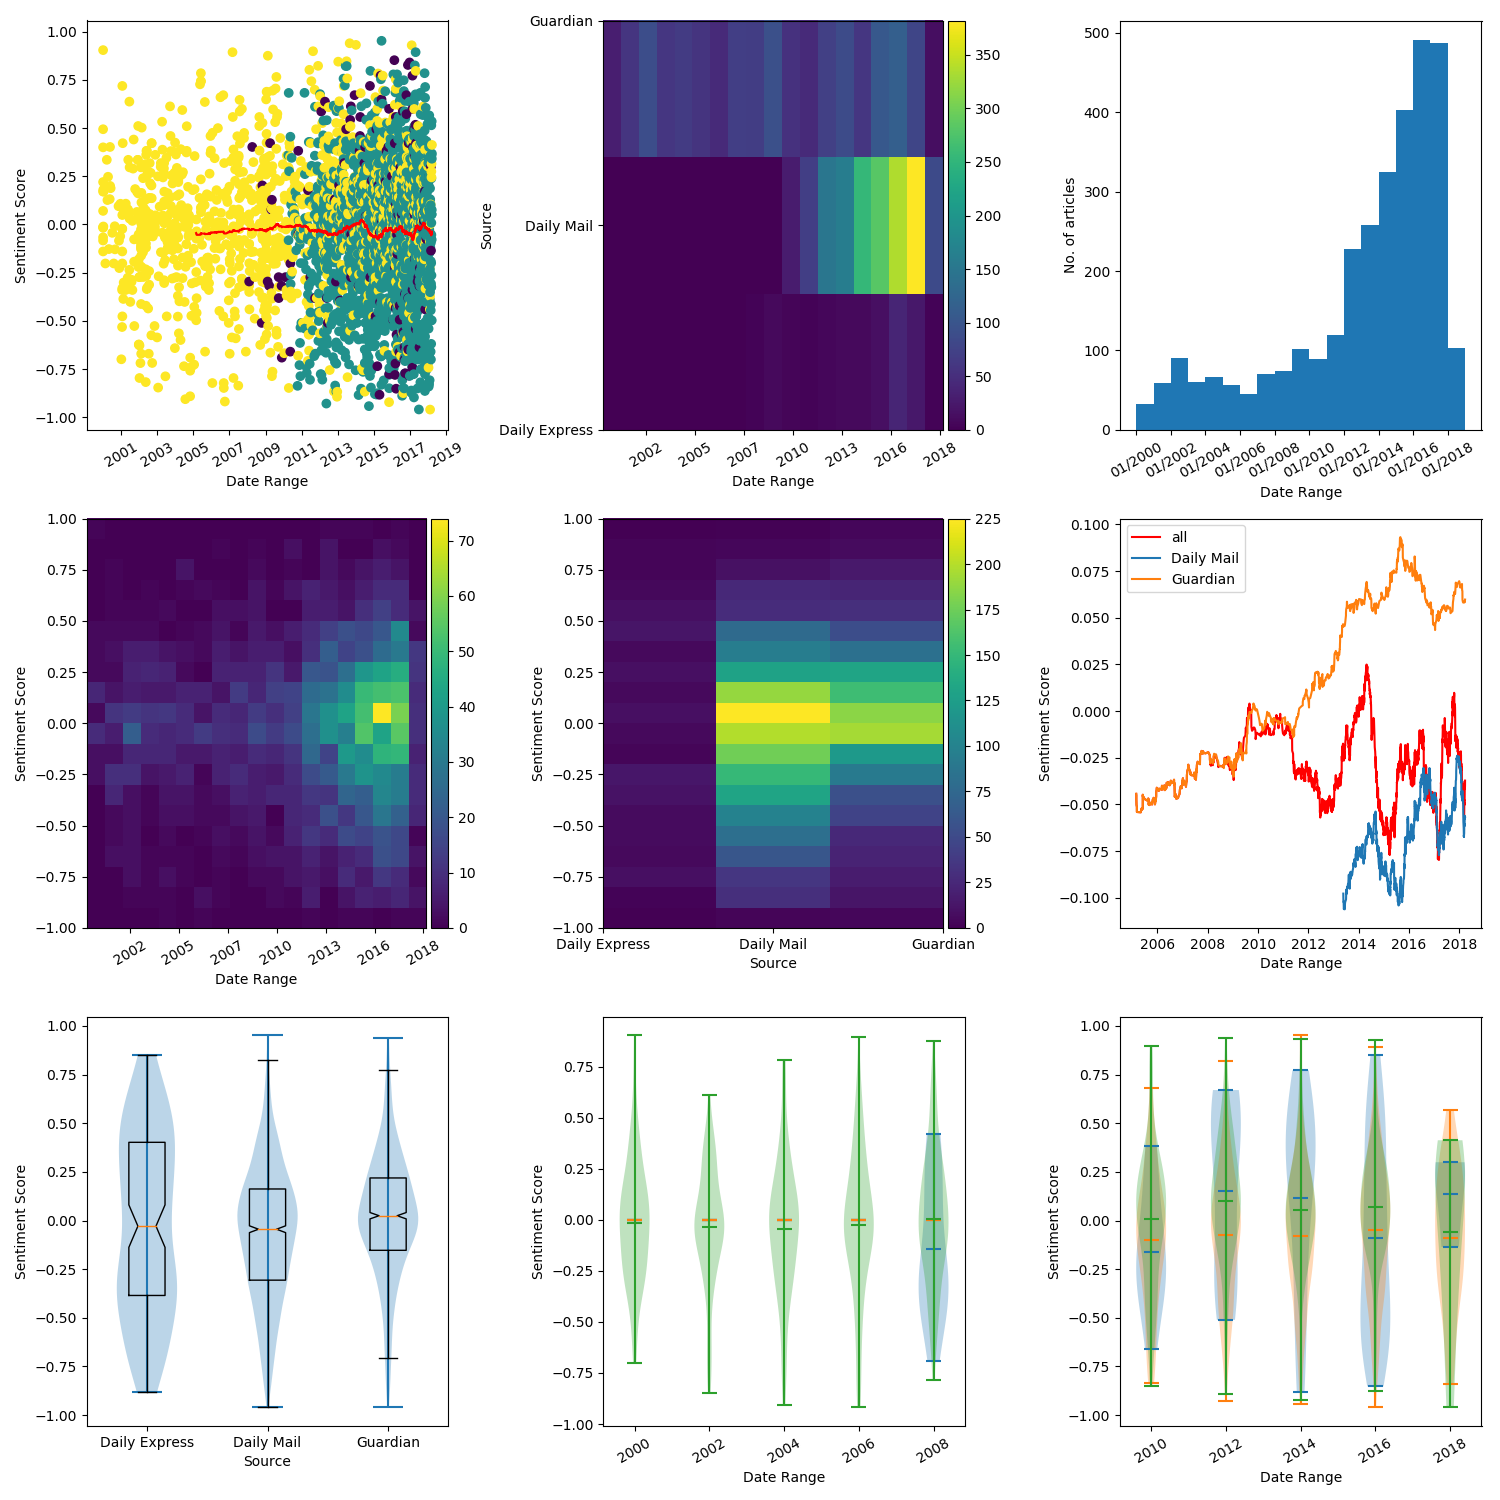
\includegraphics[width=\textwidth]{raw/autism.png}

\subsection{Mann-Whitney $U$ Test Results ($p$-values)}
\noindent
\begin{tabu} to \textwidth { | X[c] | X[c] | X[c] | X[c] | }  
	\hline
	Topic & Guardian \textgreater\space Daily Mail & Guardian \textgreater\space Daily Express & Daily Express \textgreater\space Daily Mail  \\
	\hline
	All & 3.00 * 10\textsuperscript{-12} & 0.137 & 0.184  \\
	\hline
	2010 & 0.100 & N/A & N/A  \\
	\hline
	2011 & 0.0649 & N/A & N/A  \\
	\hline
	2012 & 0.000150 & N/A & N/A  \\
	\hline
	2013 & 1.52 * 10\textsuperscript{-5} & N/A & N/A  \\
	\hline
	2014 & 0.00162 & N/A & N/A  \\
	\hline
	2015 & 0.000508 & N/A & N/A  \\
	\hline
	2016 & 0.00760 & 0.0121 & 0.0432 **  \\
	\hline
	2017 & 0.000114 & 0.0667 & 0.352  \\
	\hline
\end{tabu}

\noindent ** Indicates where the reverse assumption is true (e.g. Daily Mail \textgreater\space Daily Express instead of Daily Express \textgreater\space Daily Mail)

\subsection{Key Term Trend Plots}
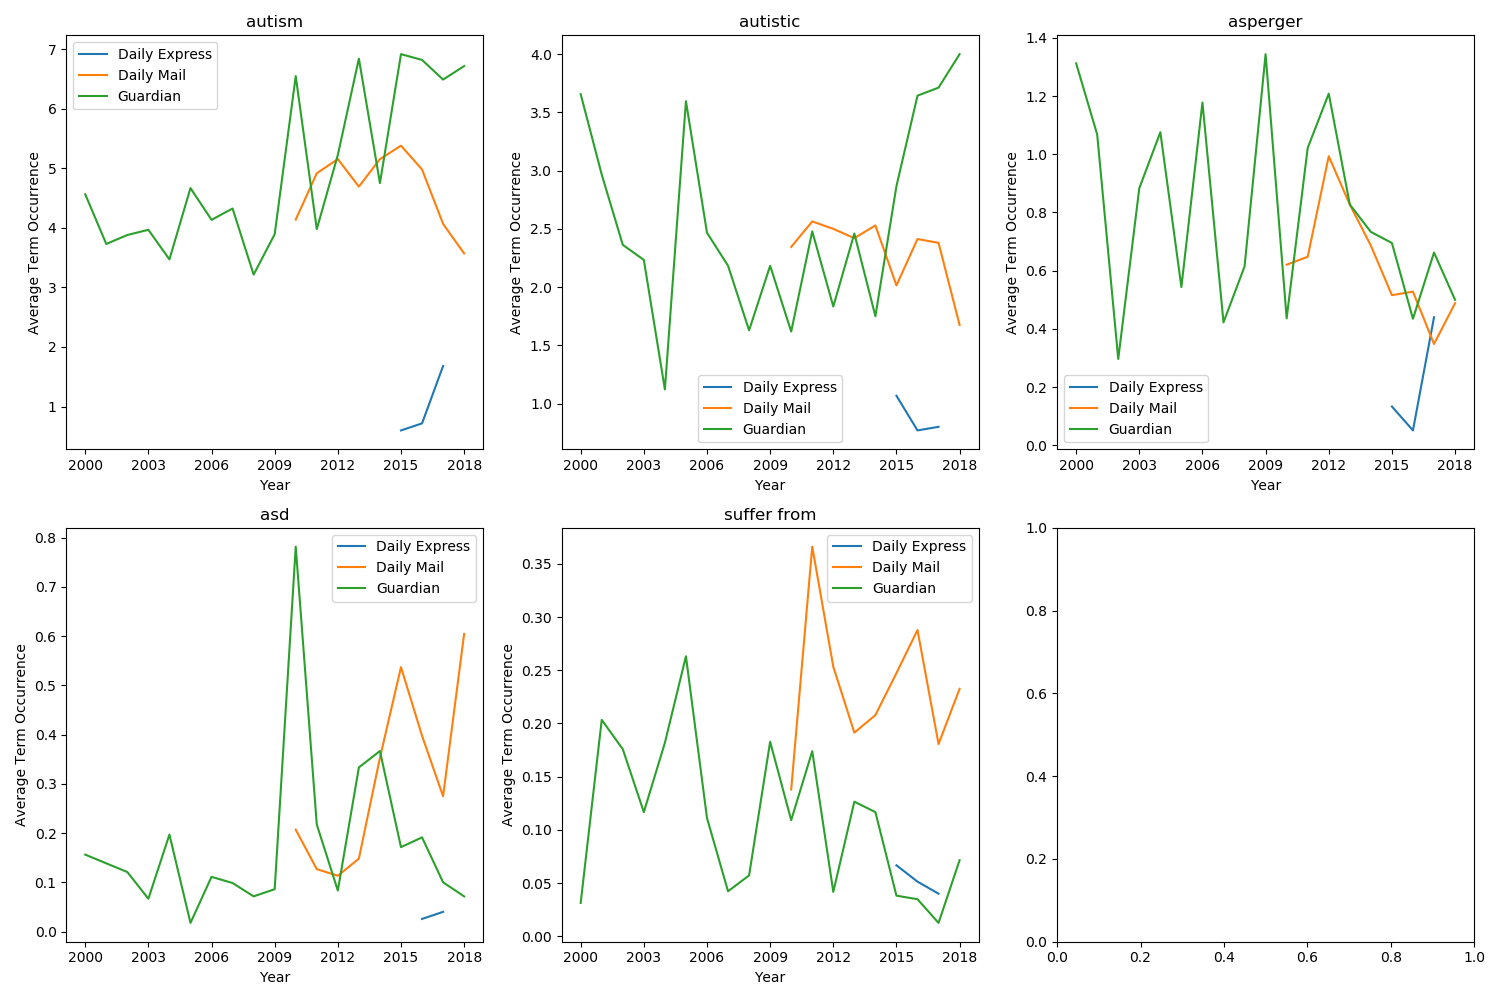
\includegraphics[width=\textwidth]{raw/autism-terms.png}

\newpage
\section{Topic: `blind'}
Key Terms: `blind', `blindness', `blindism', `visual impairment', `partially sighted', `vision loss'

\noindent Query Terms: `blind', `blindness', `visual impairment', `partially sighted', `visually impaired'

\noindent Sample size, n = 7,677

\subsection{Sentiment Score Plots}
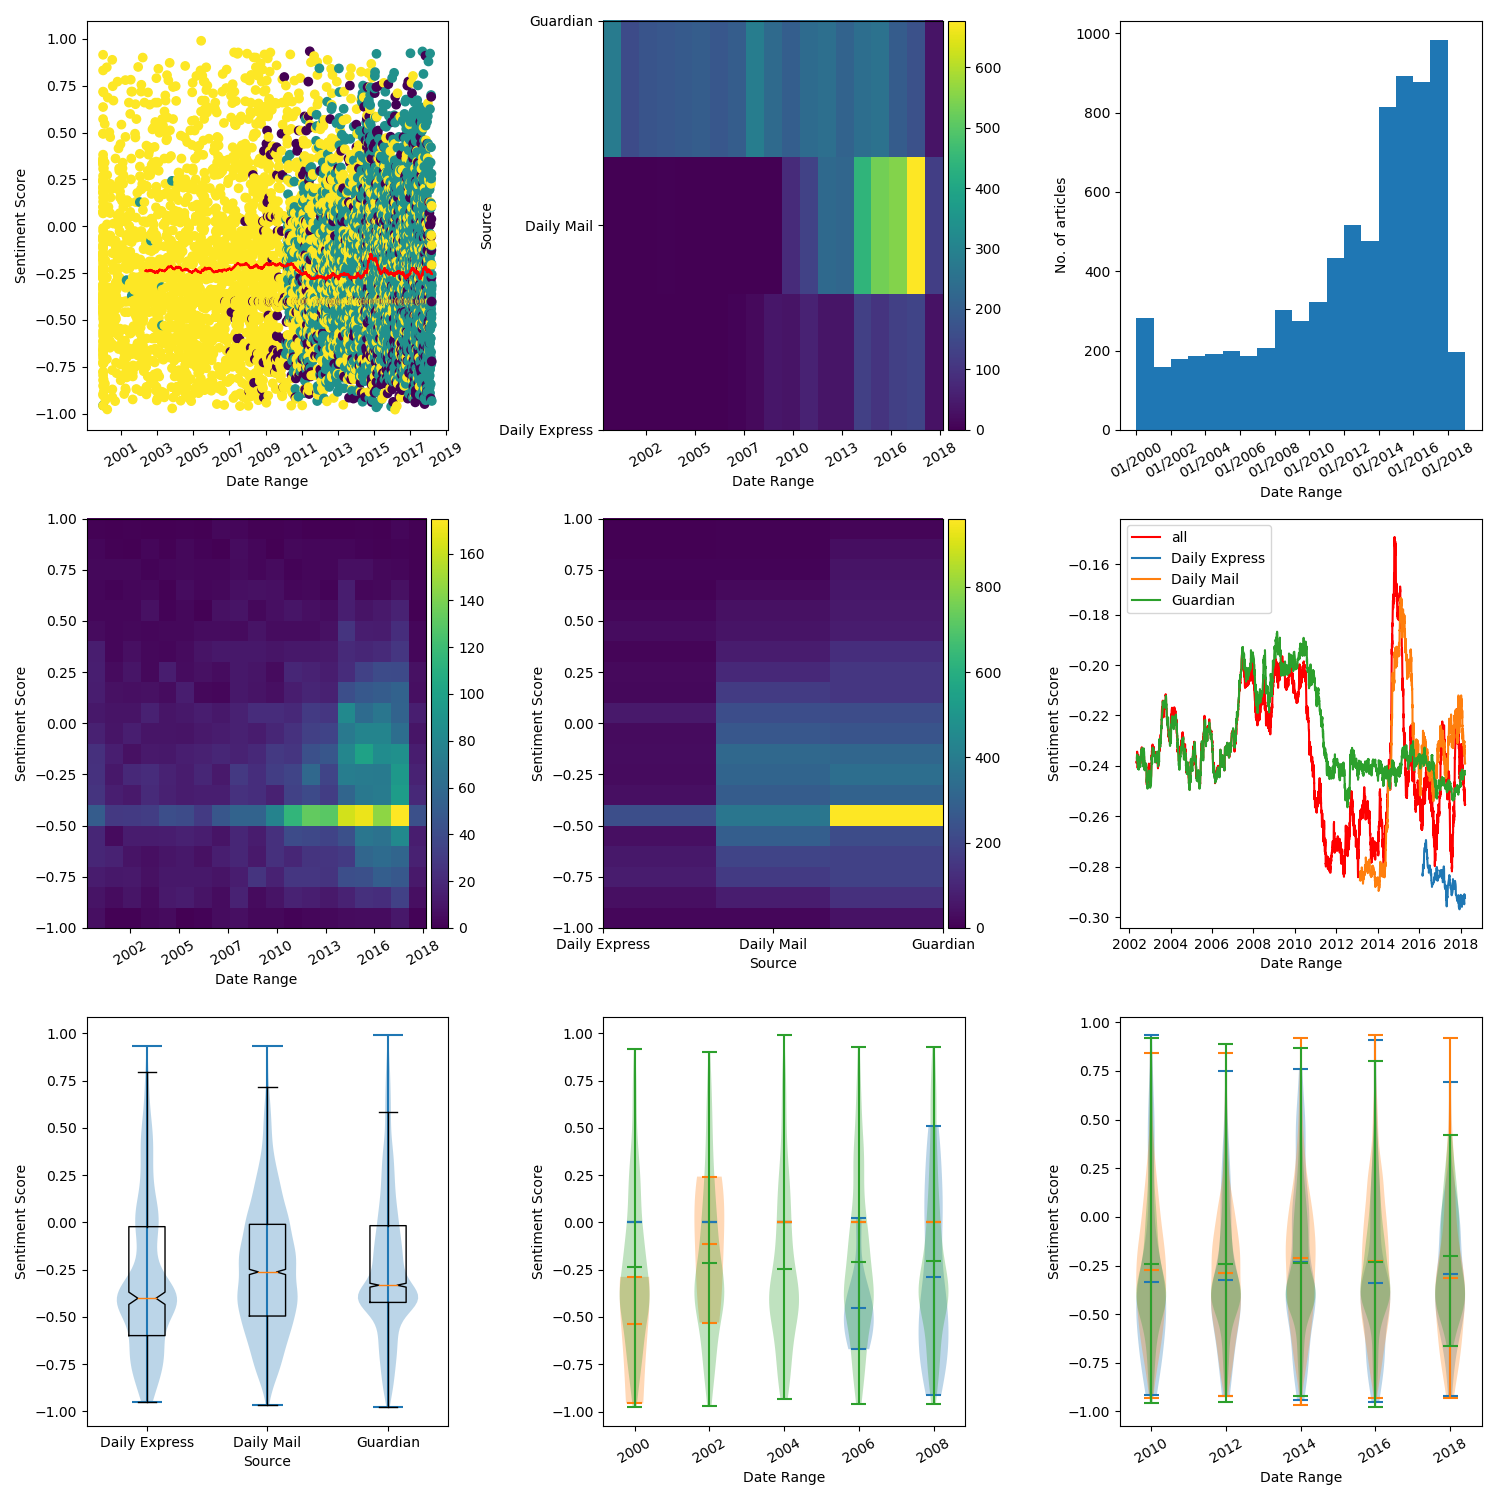
\includegraphics[width=\textwidth]{raw/blind.png}

\subsection{Mann-Whitney $U$ Test Results ($p$-values)}
\noindent
\begin{tabu} to \textwidth { | X[c] | X[c] | X[c] | X[c] | }  
	\hline
	Topic & Guardian \textgreater\space Daily Mail & Guardian \textgreater\space Daily Express & Daily Express \textgreater\space Daily Mail  \\
	\hline
	All & 0.335 ** & 1.62 * 10\textsuperscript{-9} & 6.57 * 10\textsuperscript{-9} **  \\
	\hline
	2009 & N/A & 0.339 & N/A  \\
	\hline
	2010 & 0.388 & 0.0331 & 0.0720 **  \\
	\hline
	2011 & 0.493 & 0.0101 & 0.0149 **  \\
	\hline
	2012 & 0.00585 & 0.00586 & 0.220 **  \\
	\hline
	2013 & 0.330 ** & 0.163 & 0.158 **  \\
	\hline
	2014 & 0.0670 ** & 0.263 & 0.0857 **  \\
	\hline
	2015 & 0.181 ** & 0.214 & 0.125 **  \\
	\hline
	2016 & 0.455 & 0.00119 & 0.000966 **  \\
	\hline
	2017 & 0.421 & 3.16 * 10\textsuperscript{-5} & 1.46 * 10\textsuperscript{-5} **  \\
	\hline
	2018* & 0.0118 & 0.0919 & 0.246  \\
	\hline
\end{tabu}

\noindent * 2018 data is incomplete and would only include articles up to (approximately) end of March.

\noindent ** Indicates where the reverse assumption is true (e.g. Daily Mail \textgreater\space Daily Express instead of Daily Express \textgreater\space Daily Mail)

\subsection{Key Term Trend Plots}
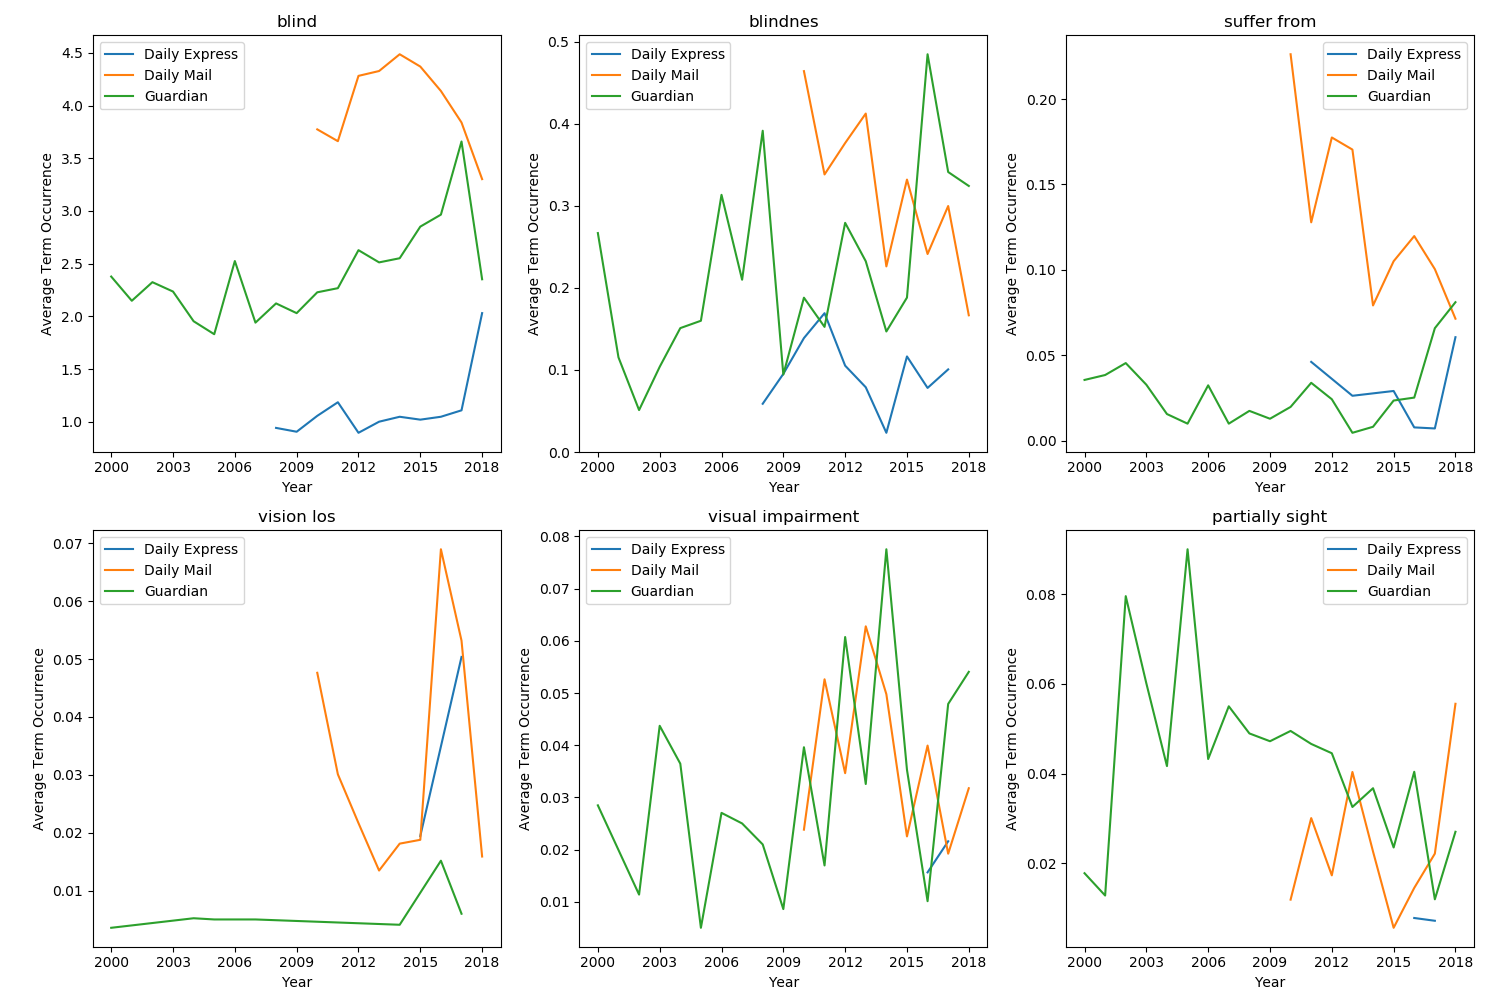
\includegraphics[width=\textwidth]{raw/blind-terms.png}

\newpage
\section{Topic: `cerebral palsy'}
Key Terms: `cerebral palsy', `spastic'

\noindent Query Terms: `cerebral palsy', `spastic'

\noindent Sample size, n = 353

\subsection{Sentiment Score Plots}
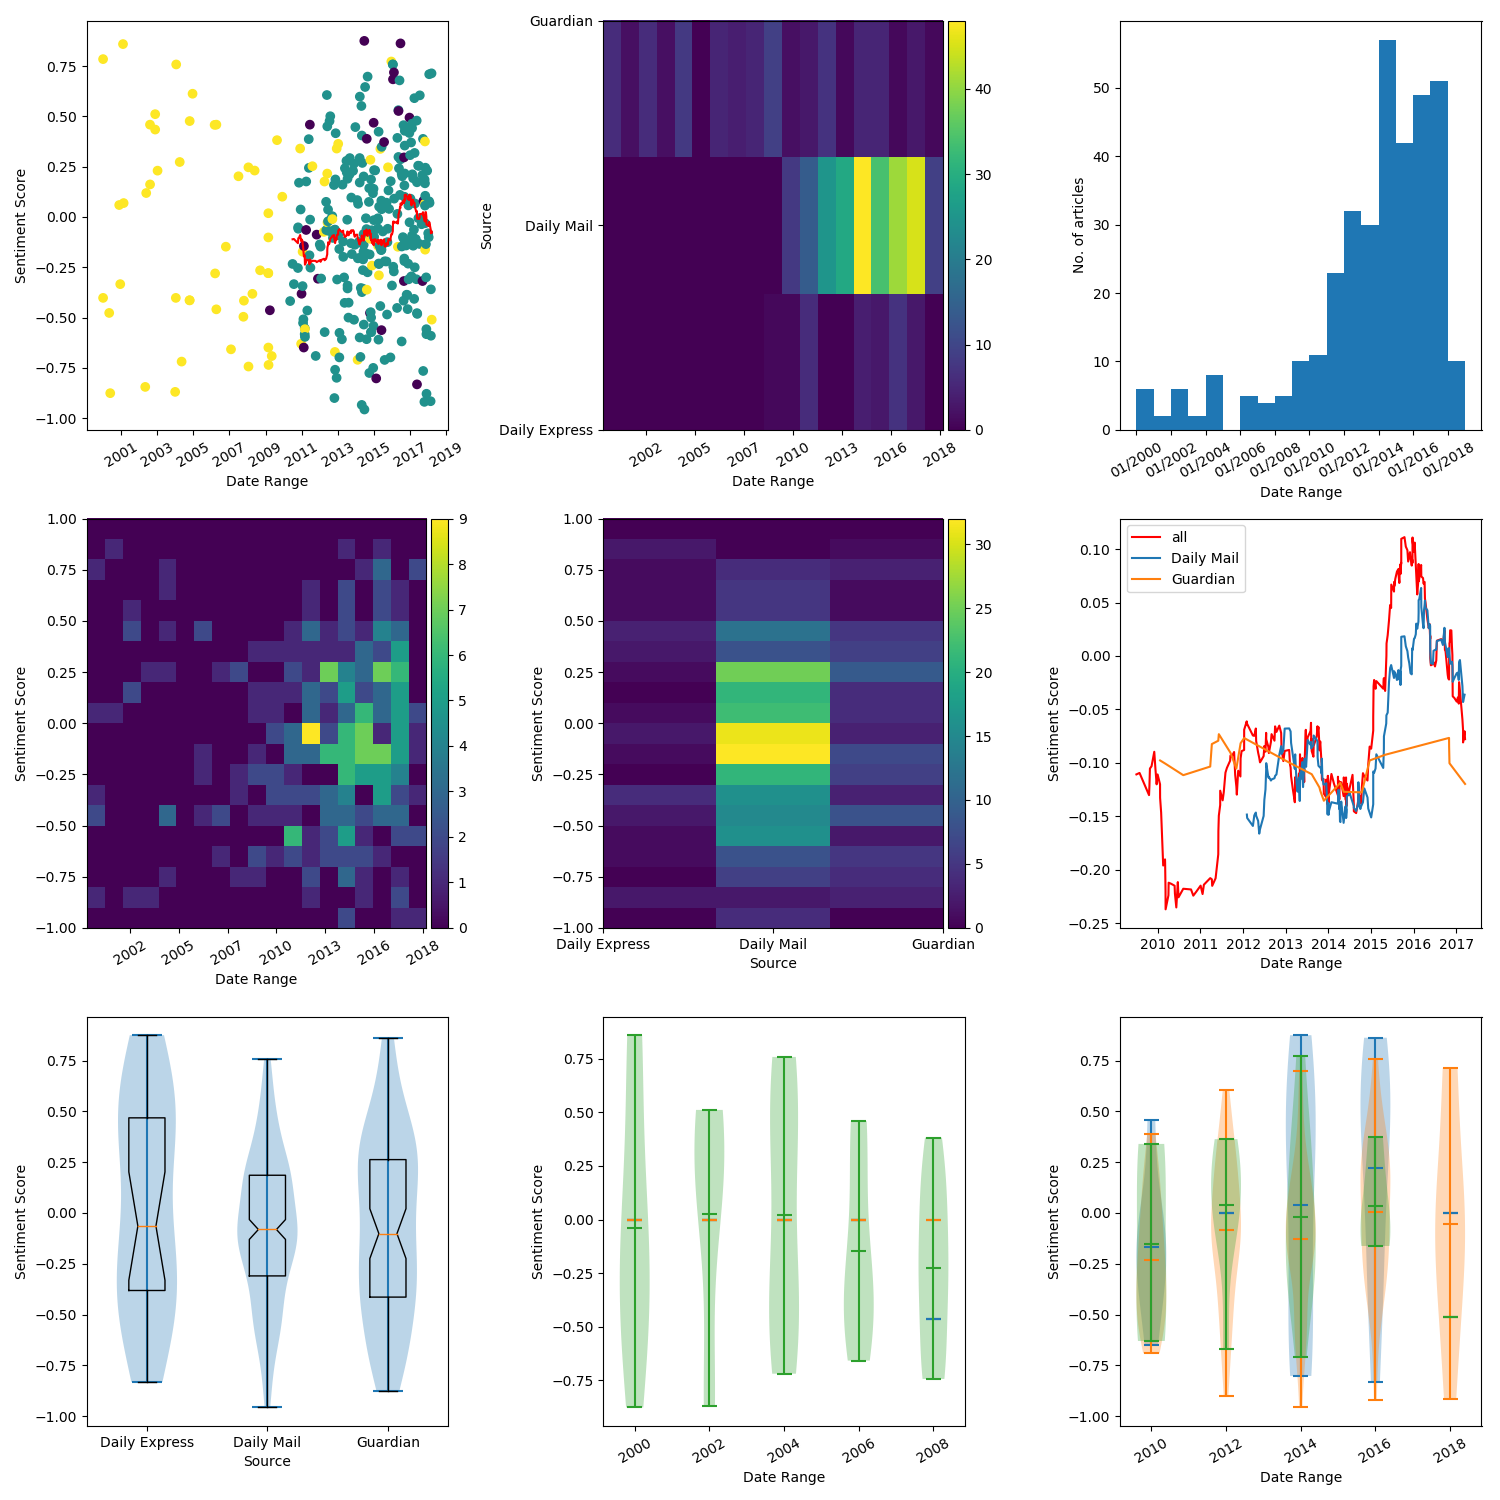
\includegraphics[width=\textwidth]{raw/cerebral-palsy.png}

\subsection{Mann-Whitney $U$ Test Results ($p$-values)}
\noindent
\begin{tabu} to \textwidth { | X[c] | X[c] | X[c] | X[c] | }  
	\hline
	Topic & Guardian \textgreater\space Daily Mail & Guardian \textgreater\space Daily Express & Daily Express \textgreater\space Daily Mail  \\
	\hline
	All & 0.469 & 0.156 ** & 0.169  \\
	\hline
\end{tabu}

\noindent Insufficient sample size for year-by-year comparisons. (n=353)

\noindent ** Indicates where the reverse assumption is true (e.g. Daily Mail \textgreater\space Daily Express instead of Daily Express \textgreater\space Daily Mail)

\subsection{Key Term Trend Plots}
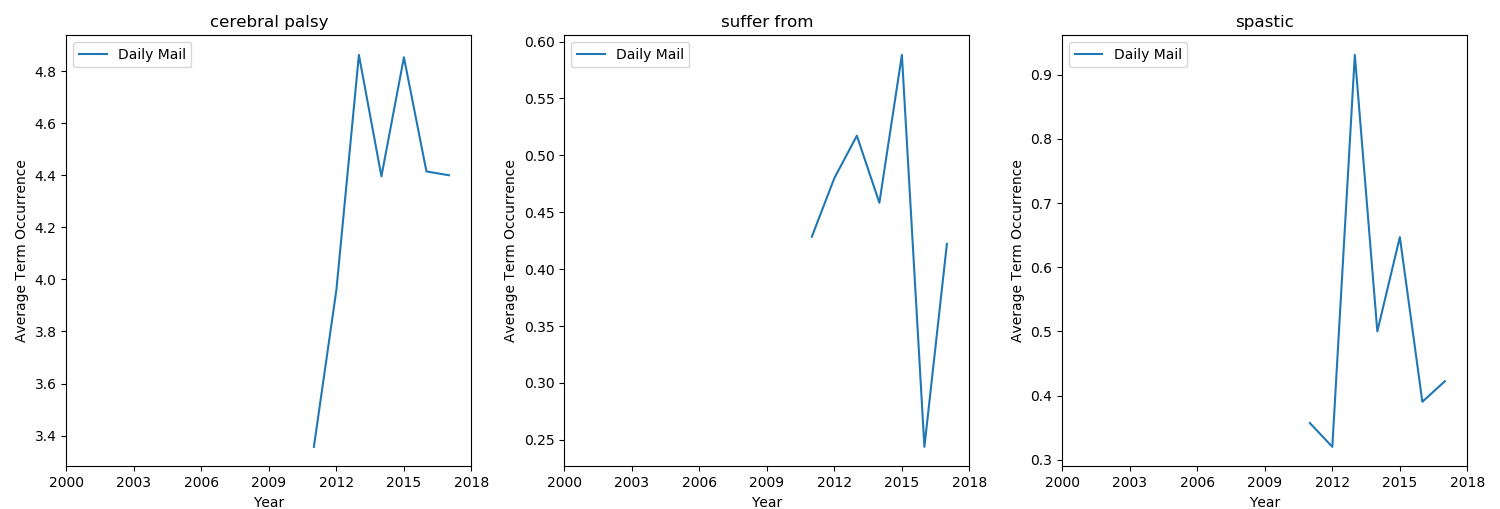
\includegraphics[width=\textwidth]{raw/cerebral-palsy-terms.png}

\newpage
\section{Topic: `deaf'}
Key Terms: `deaf', `deafness', `hearing impaired', `hard of hearing', `hearing loss'

\noindent Query Terms: `deaf', `deafness', `hearing impairment', `hard of hearing', `hearing impaired'

\noindent Sample size, n = 1,762

\subsection{Sentiment Score Plots}
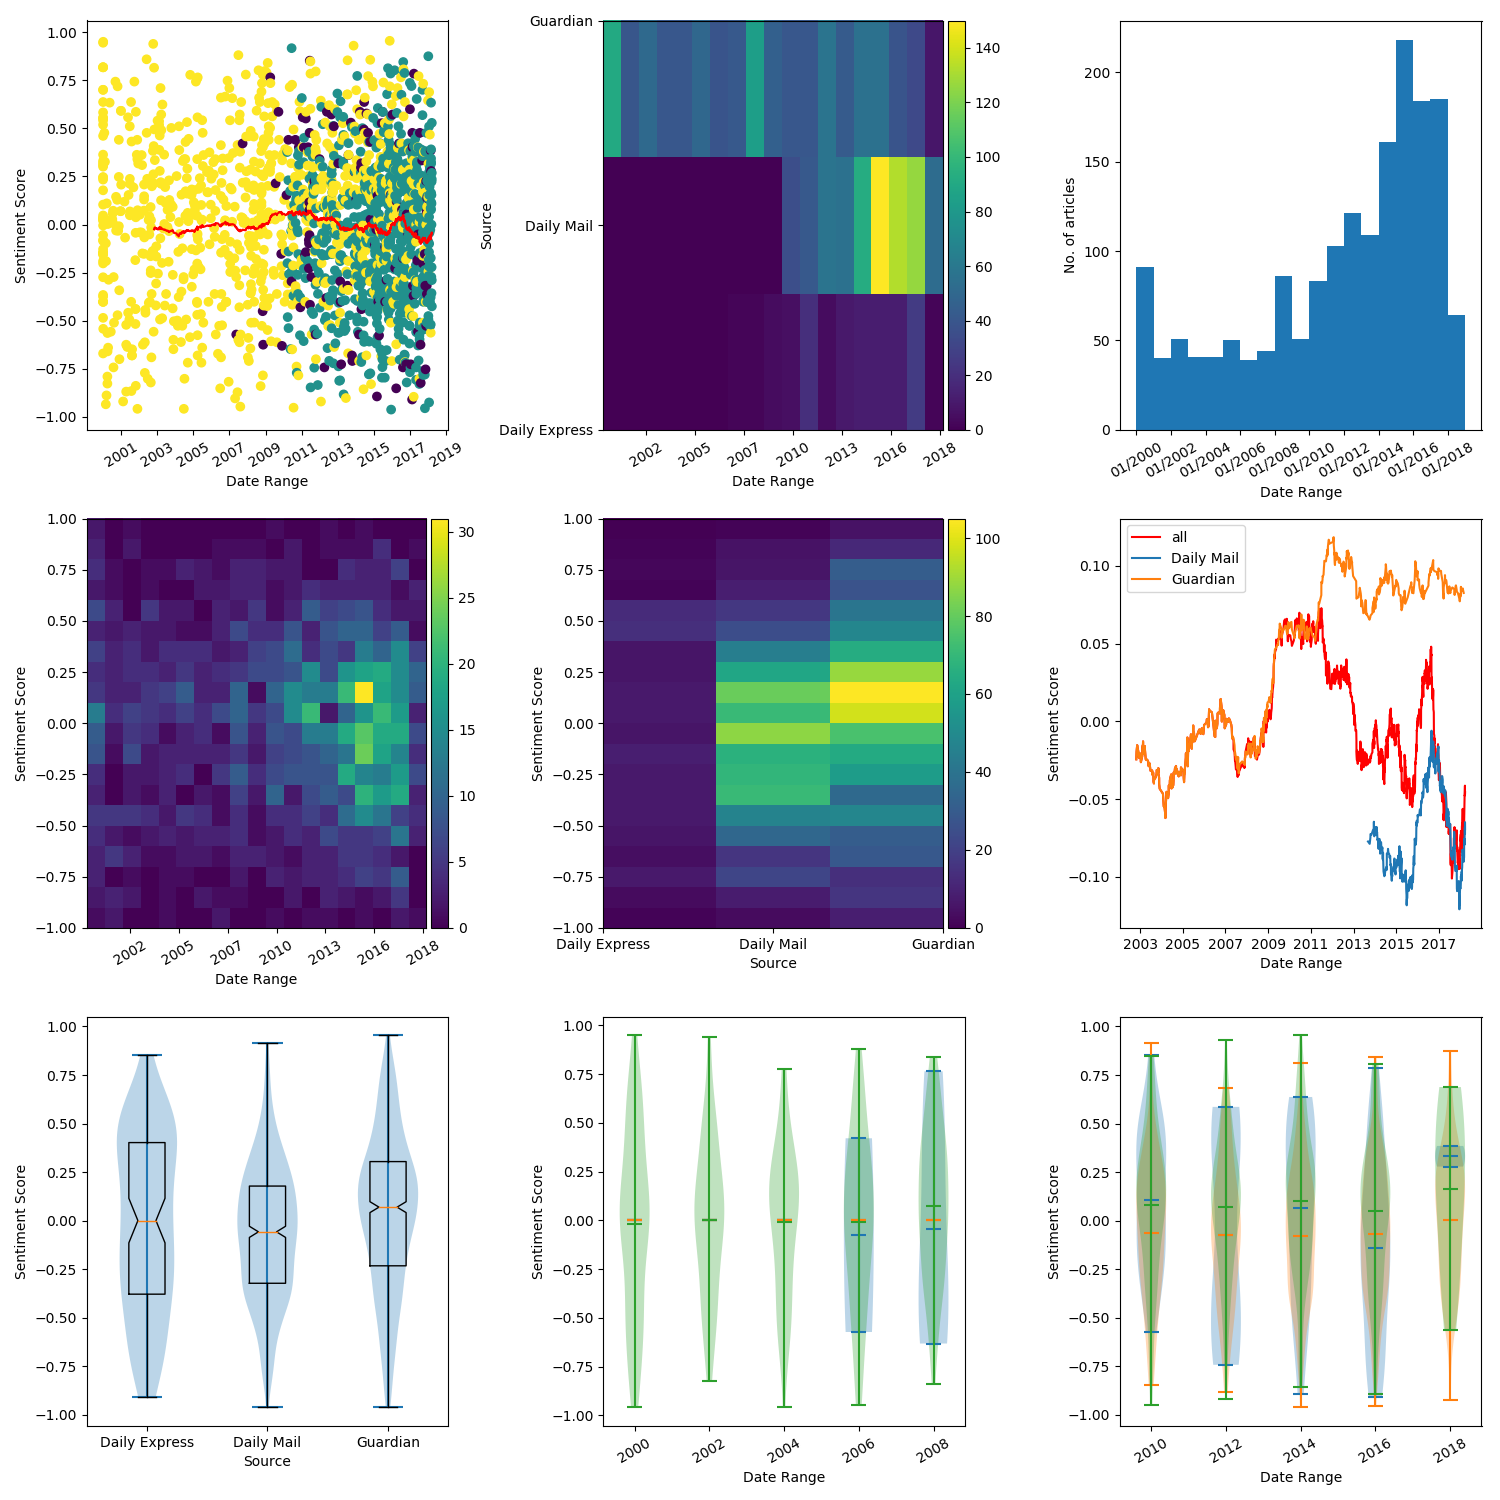
\includegraphics[width=\textwidth]{raw/deaf.png}

\subsection{Mann-Whitney $U$ Test Results ($p$-values)}
\noindent
\begin{tabu} to \textwidth { | X[c] | X[c] | X[c] | X[c] | }  
	\hline
	Topic & Guardian \textgreater\space Daily Mail & Guardian \textgreater\space Daily Express & Daily Express \textgreater\space Daily Mail  \\
	\hline
	All & 6.30 * 10\textsuperscript{-10} & 0.141 & 0.0833  \\
	\hline
	2010 & 0.263 & N/A & N/A  \\
	\hline
	2011 & 0.00262 & N/A & N/A  \\
	\hline
	2012 & 0.00349 & N/A & N/A  \\
	\hline
	2013 & 0.0403 & N/A & N/A  \\
	\hline
	2014 & 0.000131 & N/A & N/A  \\
	\hline
	2015 & 0.00260 & N/A & N/A  \\
	\hline
	2016 & 0.0437 & N/A & N/A  \\
	\hline
	2017 & 0.0307 & 0.0480 & 0.233 **  \\
	\hline
\end{tabu}

\noindent ** Indicates where the reverse assumption is true (e.g. Daily Mail \textgreater\space Daily Express instead of Daily Express \textgreater\space Daily Mail)

\subsection{Key Term Trend Plots}
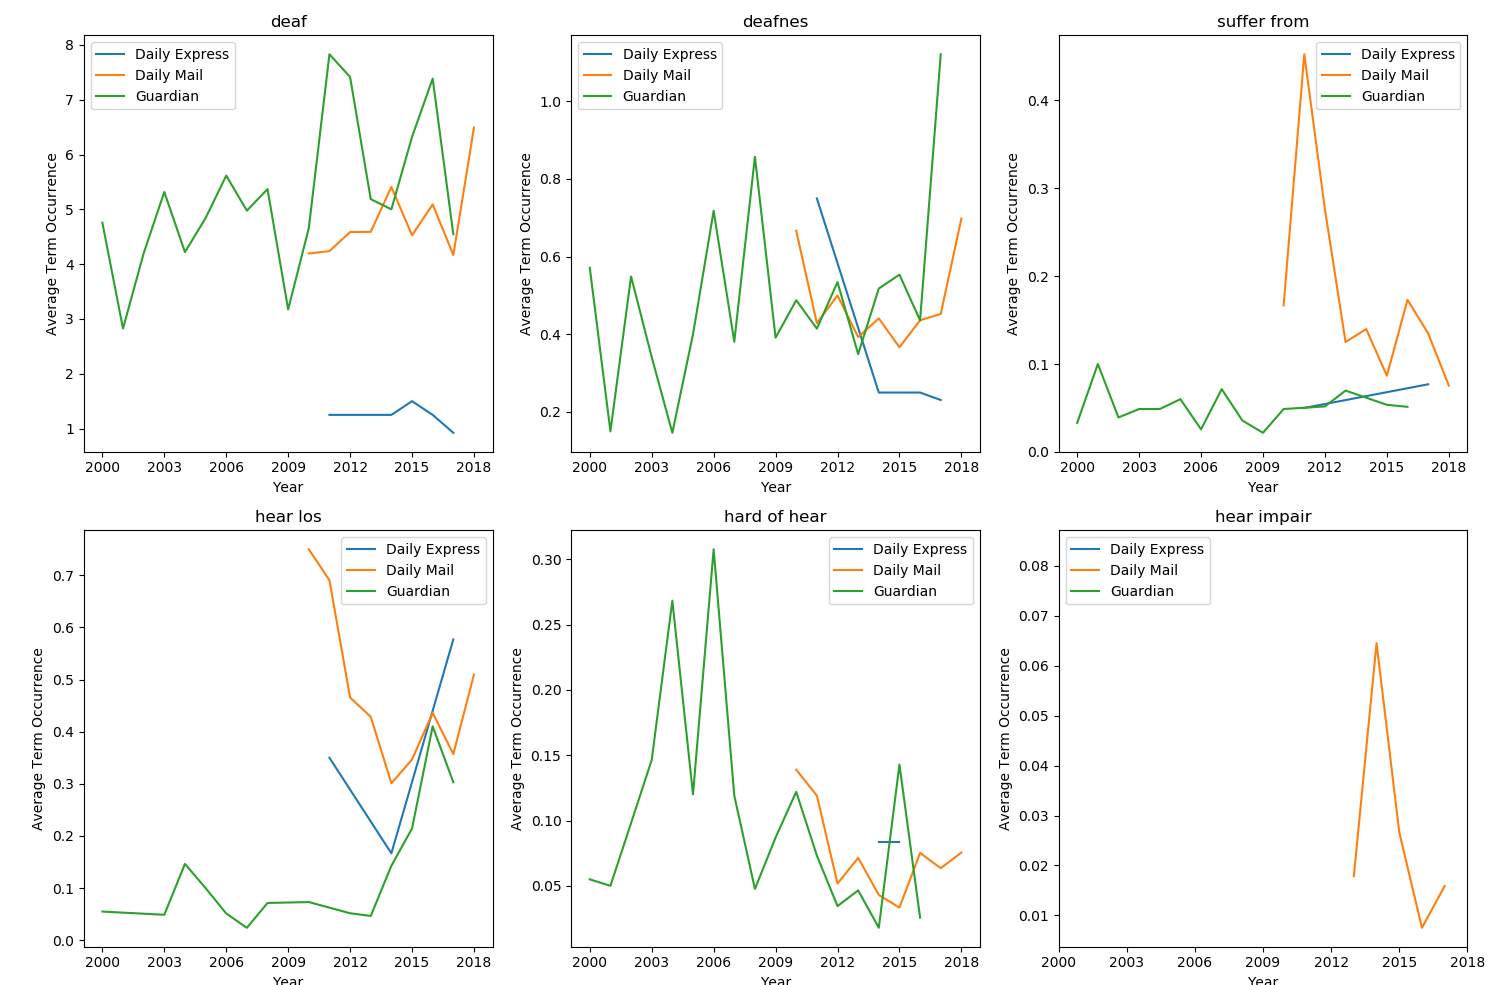
\includegraphics[width=\textwidth]{raw/deaf-terms.png}

\newpage
\section{Topic: `developmental delay'}
Key Terms: `developmental delay', `developmental disability', `developmental disorder', `learning disability', `slow learner', `intellectual disability'

\noindent Query Terms: `developmental delay', `developmental disability', `developmental disorder', `learning disability'

\subsection{Sentiment Score Plots}
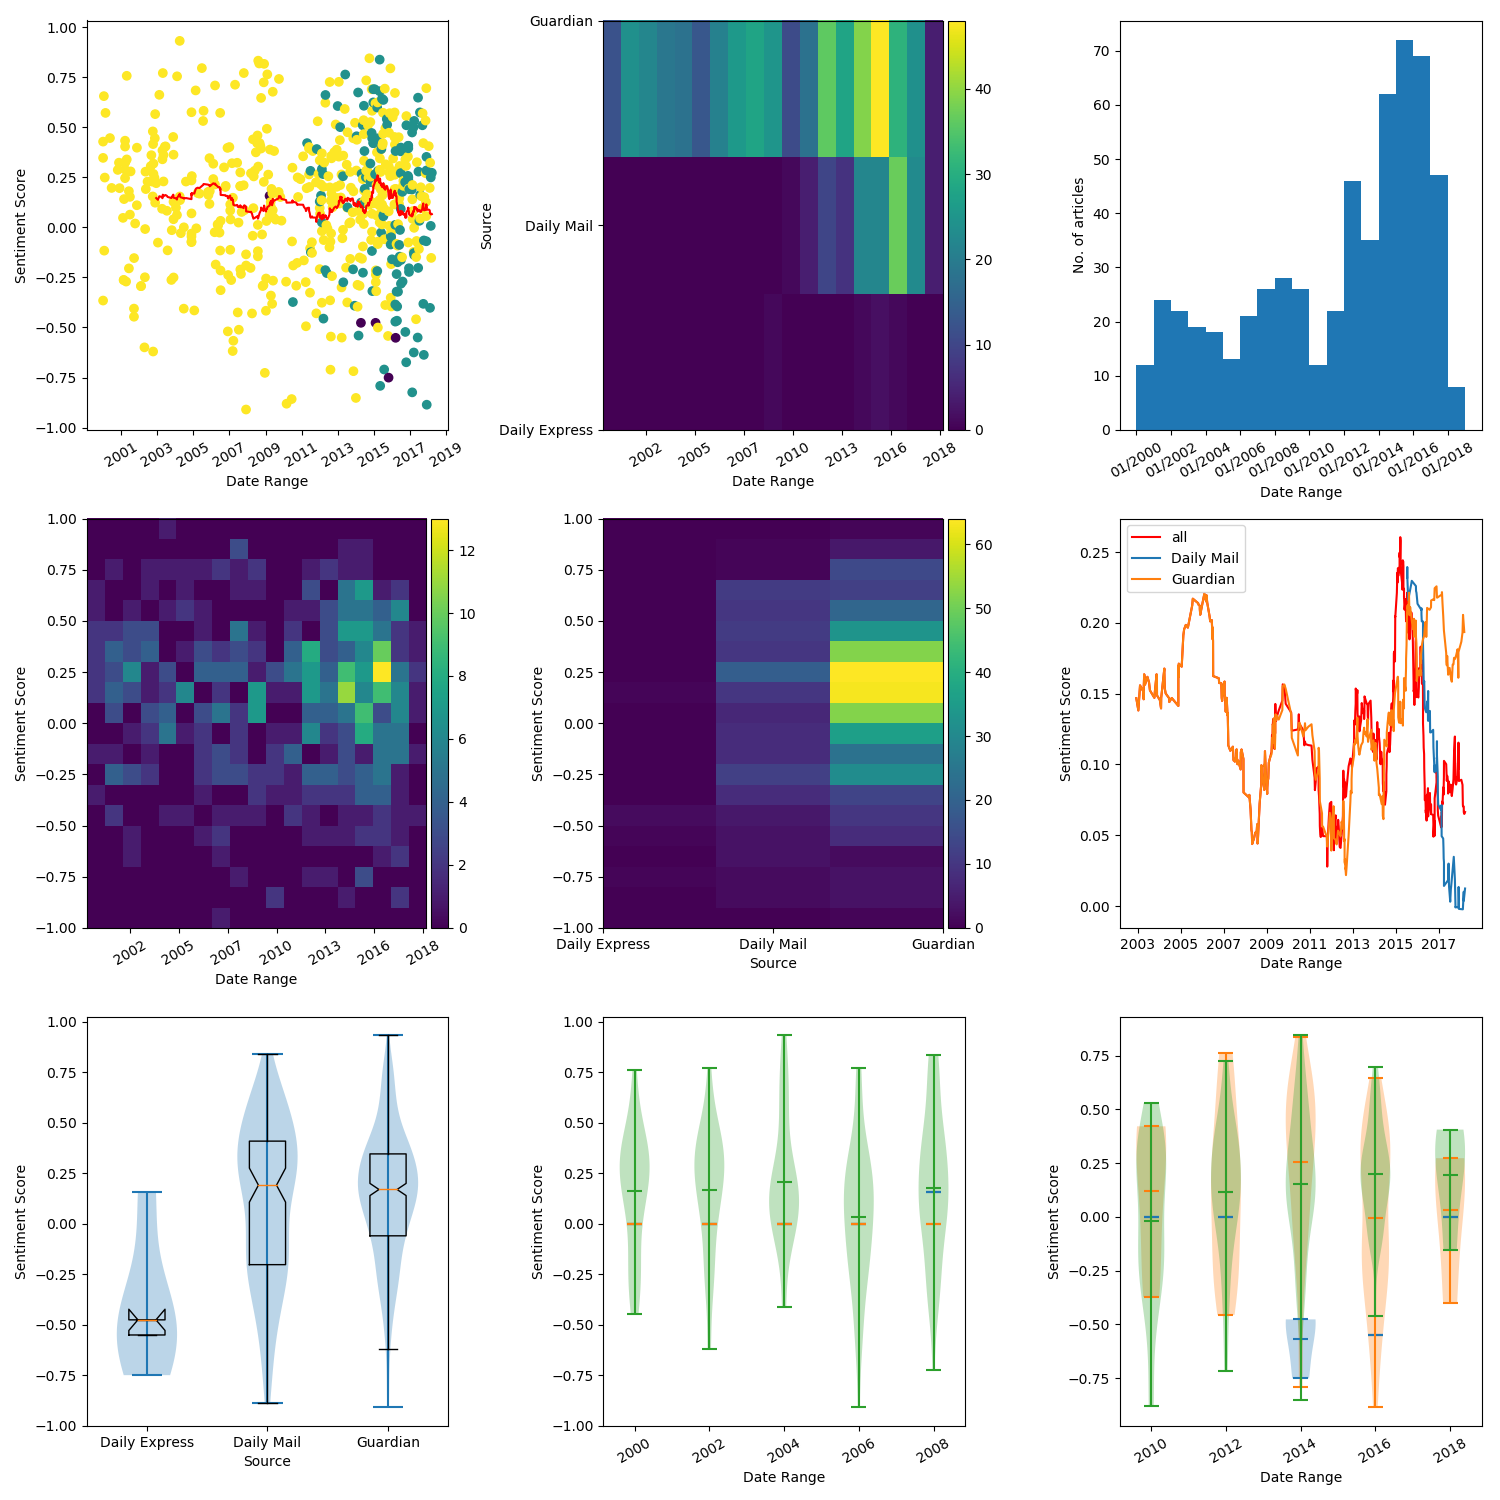
\includegraphics[width=\textwidth]{raw/developmental-delay.png}

\noindent Sample size, n = 582

\subsection{Mann-Whitney $U$ Test Results ($p$-values)}
\noindent
\begin{tabu} to \textwidth { | X[c] | X[c] | X[c] | X[c] | }  
	\hline
	Topic & Guardian \textgreater\space Daily Mail & Guardian \textgreater\space Daily Express & Daily Express \textgreater\space Daily Mail  \\
	\hline
	All & 0.383 & 0.00179 & 0.00326 **  \\
	\hline
	2014 & 0.0695 ** & N/A & N/A  \\
	\hline
	2015 & 0.106 ** & N/A & N/A  \\
	\hline
	2016 & 0.000845 & N/A & N/A  \\
	\hline
	2017 & 0.251 & N/A & N/A  \\
	\hline
\end{tabu}

\noindent ** Indicates where the reverse assumption is true (e.g. Daily Mail \textgreater\space Daily Express instead of Daily Express \textgreater\space Daily Mail)

\subsection{Key Term Trend Plots}
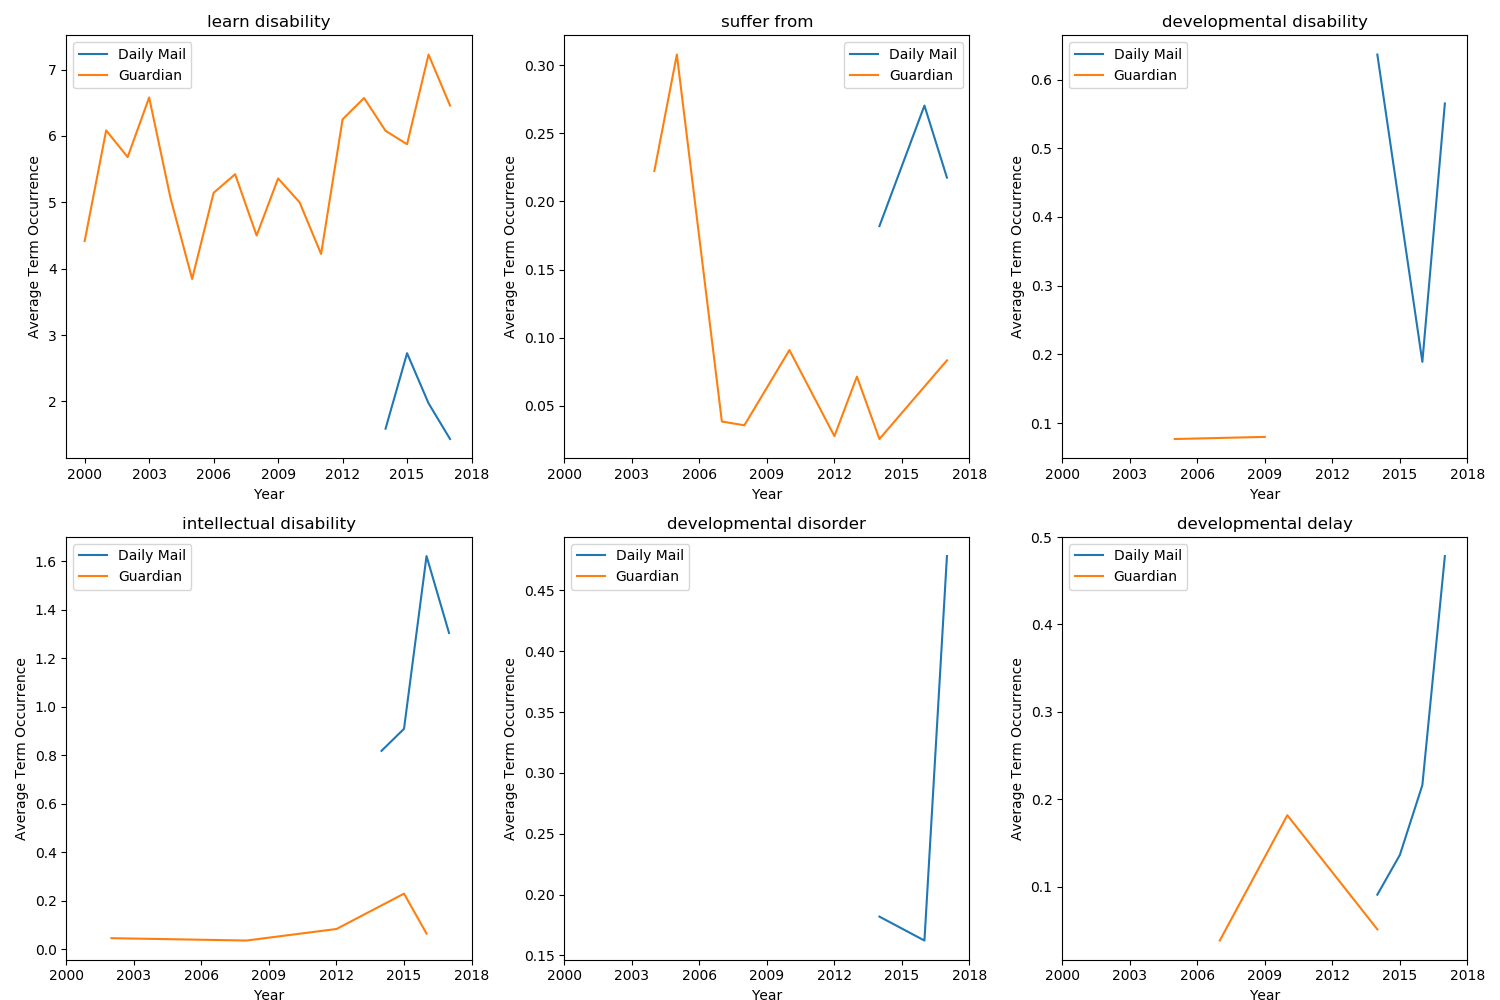
\includegraphics[width=\textwidth]{raw/developmental-delay-terms.png}

\newpage
\section{Topic: `dyslexia'}
Key Terms: `dyslexia', `dyslexic'

\noindent Query Terms: `dyslexia', `dyslexic'

\noindent Sample size, n = 410

\subsection{Sentiment Score Plots}
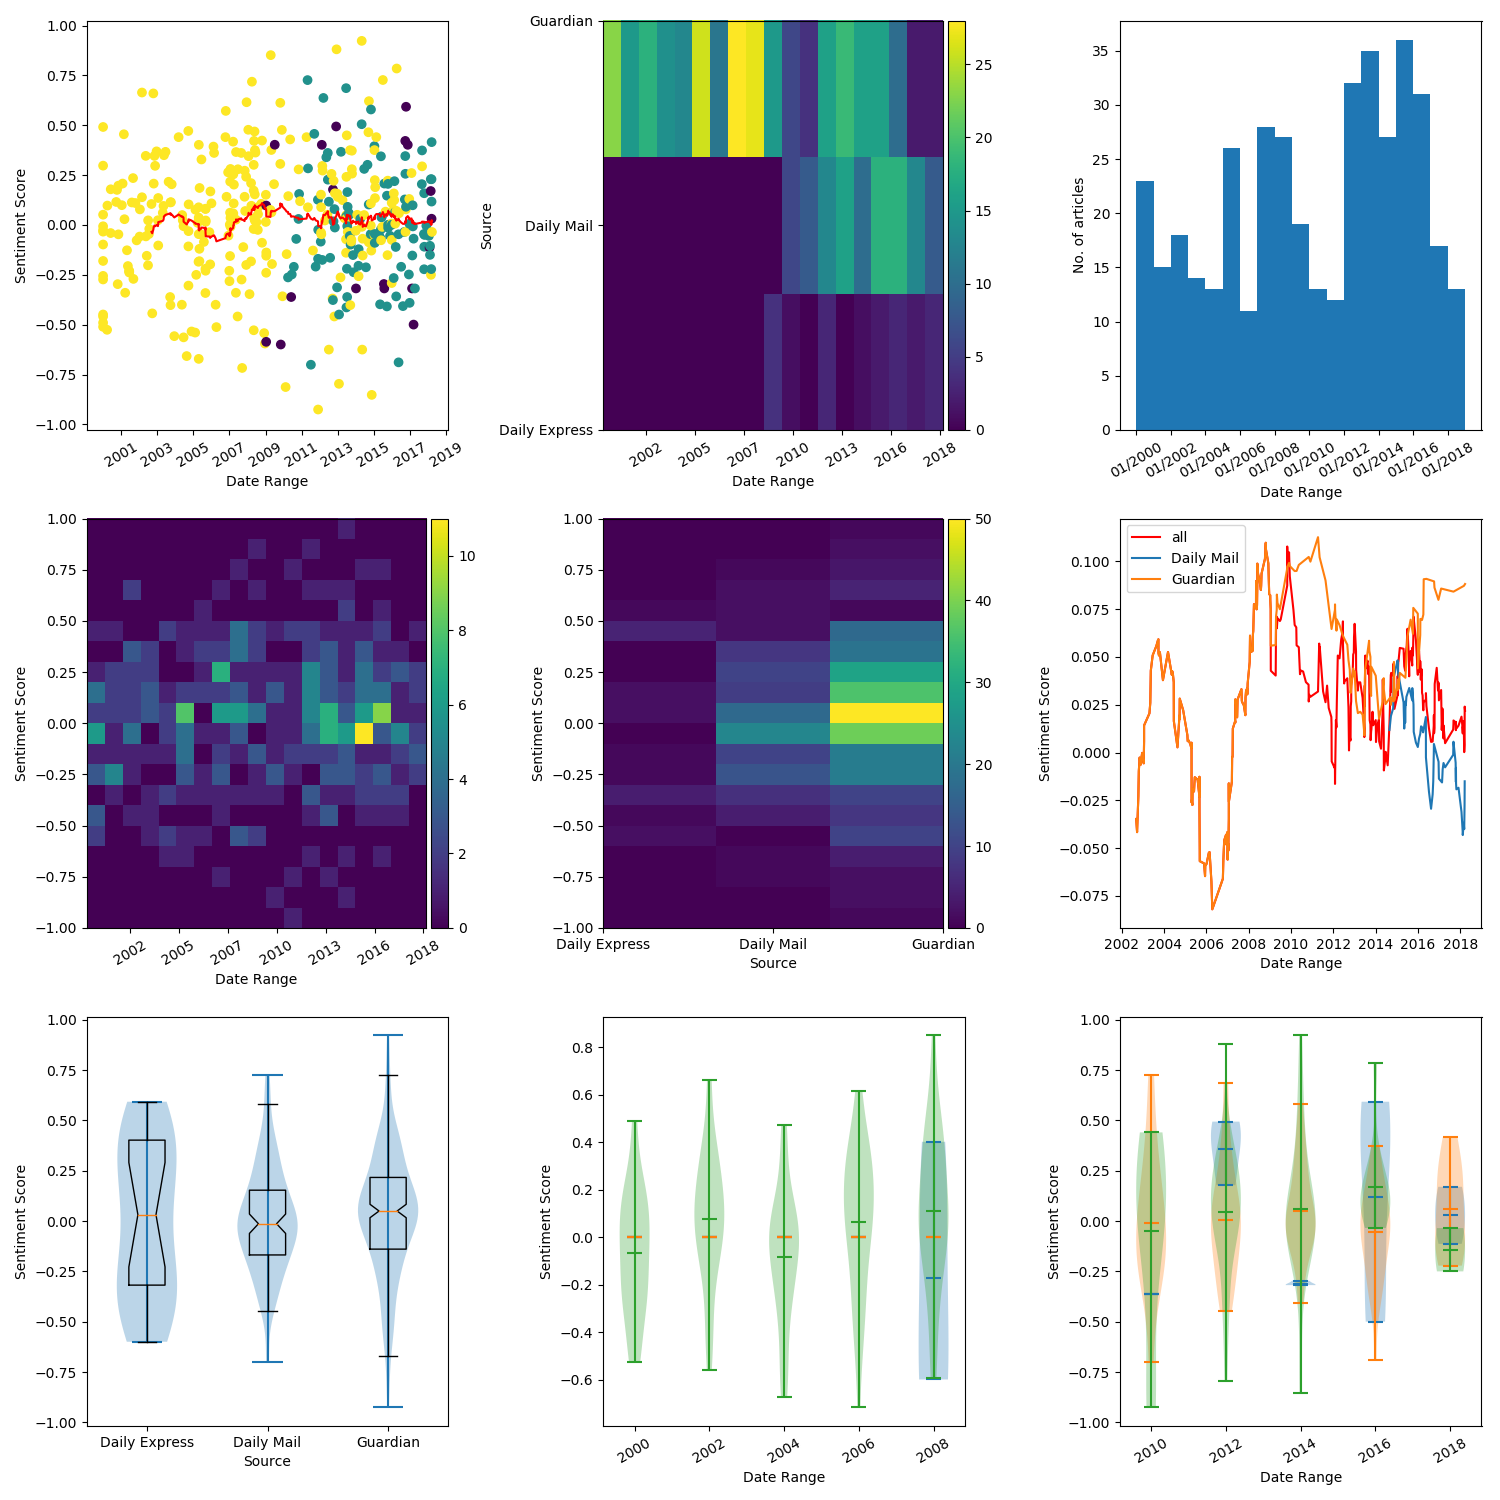
\includegraphics[width=\textwidth]{raw/dyslexia.png}

\subsection{Mann-Whitney $U$ Test Results ($p$-values)}
\noindent
\begin{tabu} to \textwidth { | X[c] | X[c] | X[c] | X[c] | }  
	\hline
	Topic & Guardian \textgreater\space Daily Mail & Guardian \textgreater\space Daily Express & Daily Express \textgreater\space Daily Mail  \\
	\hline
	All & 0.0740 & 0.362 & 0.464 **  \\
	\hline
\end{tabu}

\noindent Insufficient sample size for year-by-year comparisons. (n=410).

\noindent ** Indicates where the reverse assumption is true (e.g. Daily Mail \textgreater\space Daily Express instead of Daily Express \textgreater\space Daily Mail)

\subsection{Key Term Trend Plots}
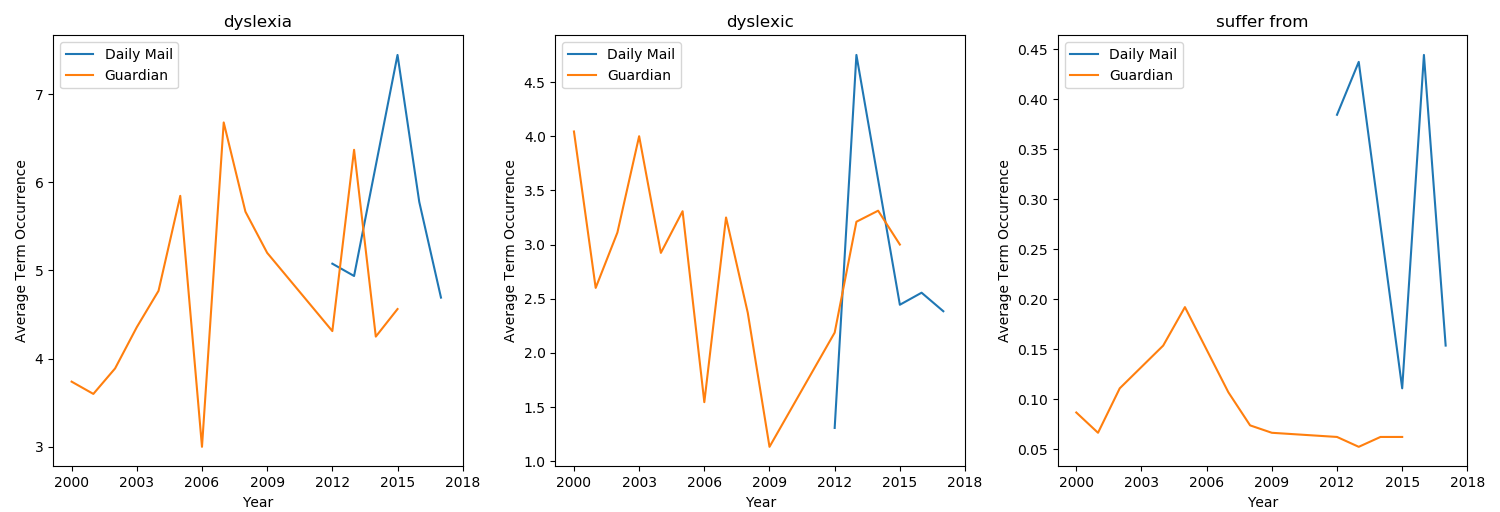
\includegraphics[width=\textwidth]{raw/dyslexia-terms.png}

\newpage
\section{Topic: `epilepsy'}
Key Terms: `epilepsy', `epileptic', `seizure'

\noindent Query Terms: `epilepsy', `epileptic'

\subsection{Sentiment Score Plots}
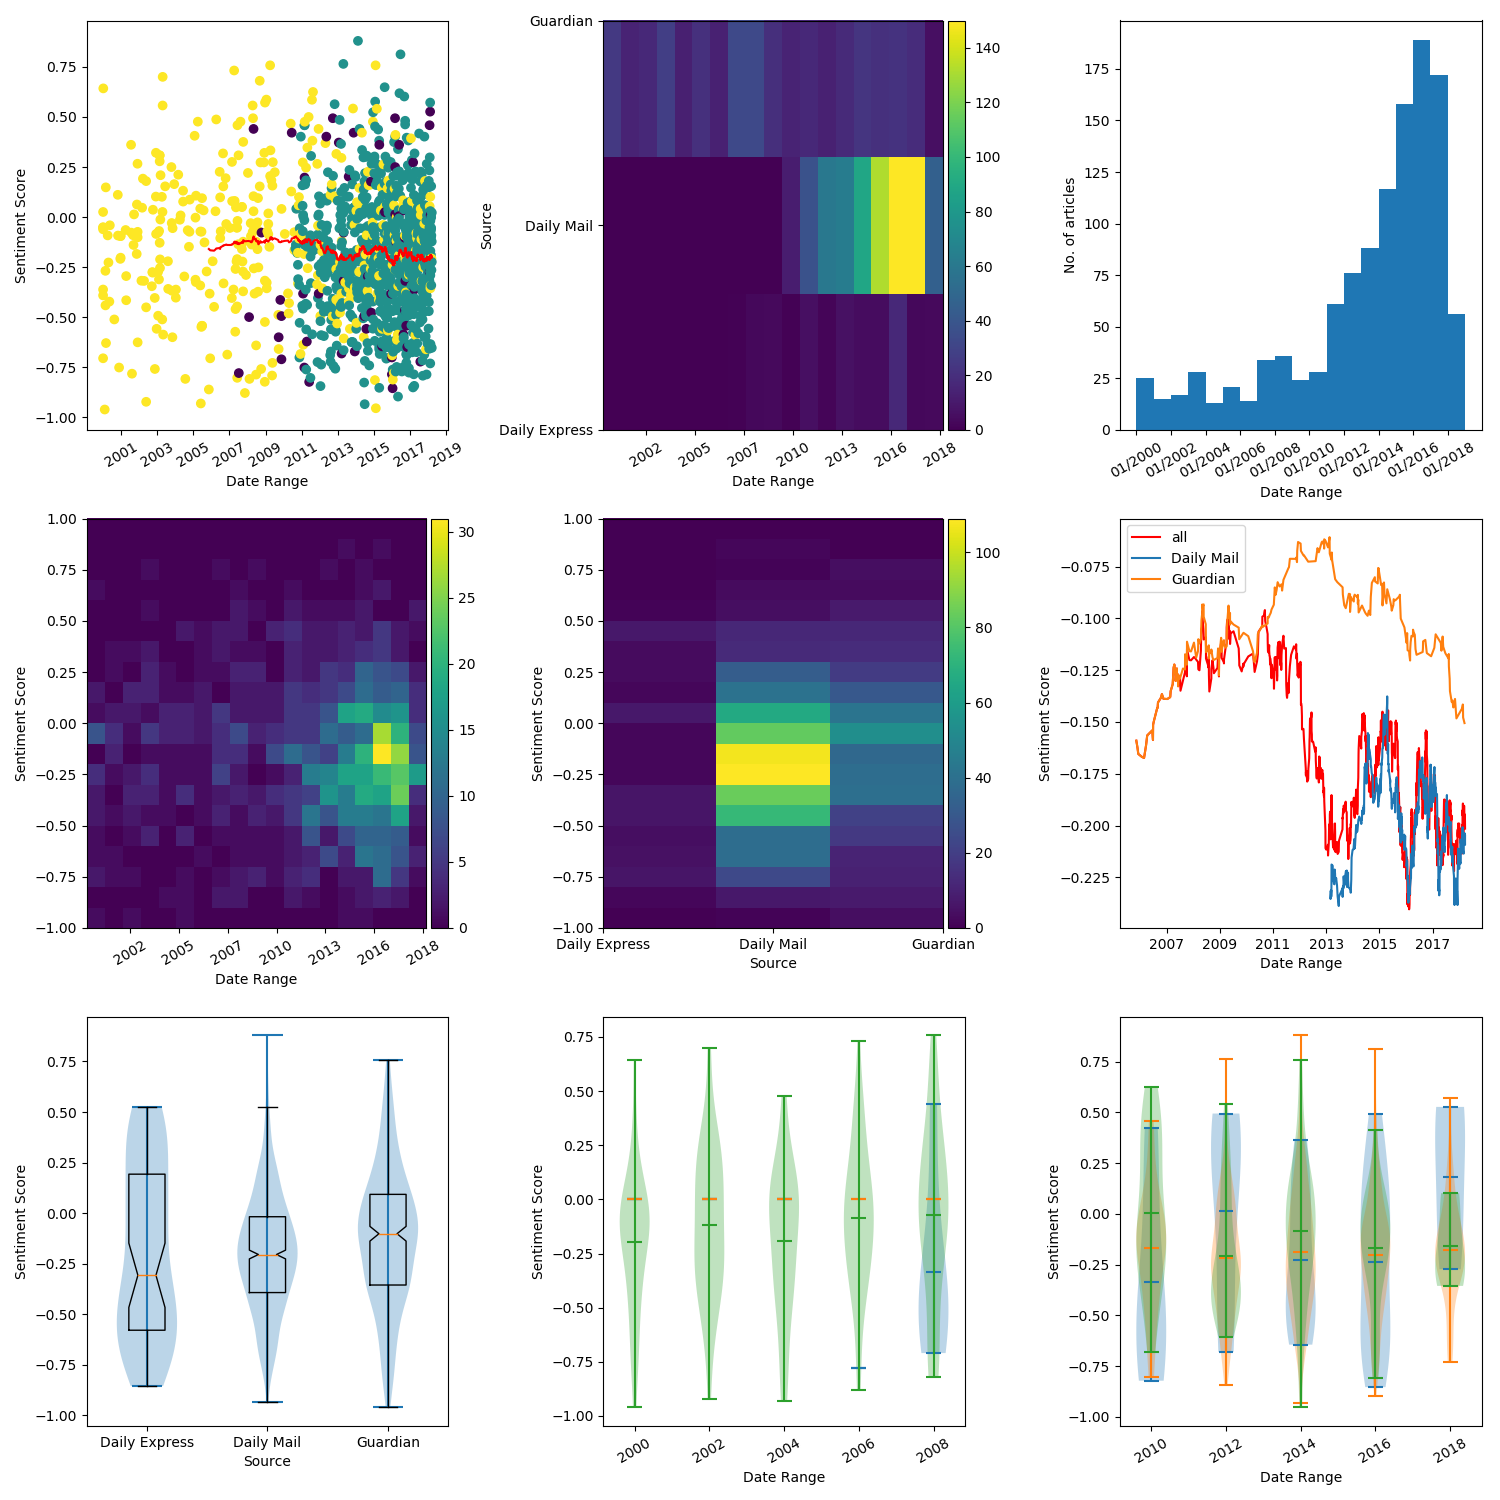
\includegraphics[width=\textwidth]{raw/epilepsy.png}

\noindent Sample size, n = 1,172

\subsection{Mann-Whitney $U$ Test Results ($p$-values)}
\noindent
\begin{tabu} to \textwidth { | X[c] | X[c] | X[c] | X[c] | }  
	\hline
	Topic & Guardian \textgreater\space Daily Mail & Guardian \textgreater\space Daily Express & Daily Express \textgreater\space Daily Mail  \\
	\hline
	All & 3.39 * 10\textsuperscript{-5} & 0.0579 & 0.322 **  \\
	\hline
	2014 & 0.0130 & N/A & N/A  \\
	\hline
	2015 & 0.193 & N/A & N/A  \\
	\hline
	2016 & 0.398 ** & N/A & N/A  \\
	\hline
\end{tabu}

\noindent ** Indicates where the reverse assumption is true (e.g. Daily Mail \textgreater\space Daily Express instead of Daily Express \textgreater\space Daily Mail)

\subsection{Key Term Trend Plots}
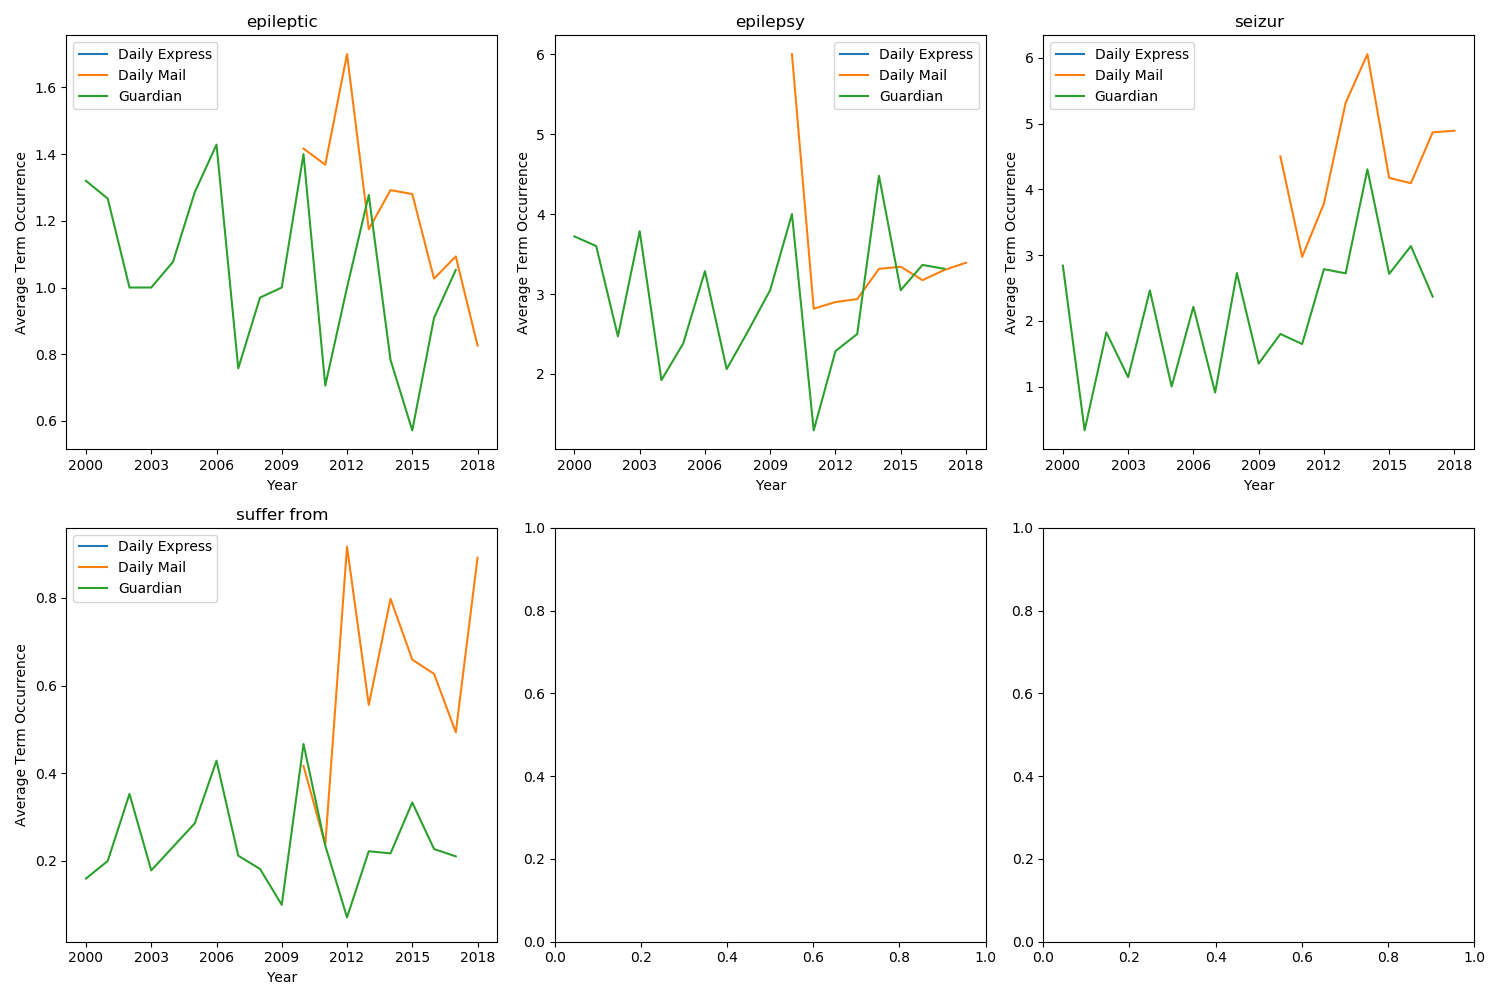
\includegraphics[width=\textwidth]{raw/epilepsy-terms.png}

\newpage
\section{Topic: `mental illness'}
Key Terms: `mental illness', `mental health', `mental disability', `mental disorder', `mental issue', `brain injured', `brain injury', `brain damaged', `psychological', `psychiatric', `emotional disorder', `behavioural disorder', `retardation', `intellectual disability', `mentally ill', `mentally disabled', `mentally handicapped'

\noindent Query Terms: `mental illness', `mental health', `mental disorder', `mental disability', `mentally ill', `mentally disabled', `mentally handicapped'

\noindent Sample size, n = 15,329

\subsection{Sentiment Score Plots}
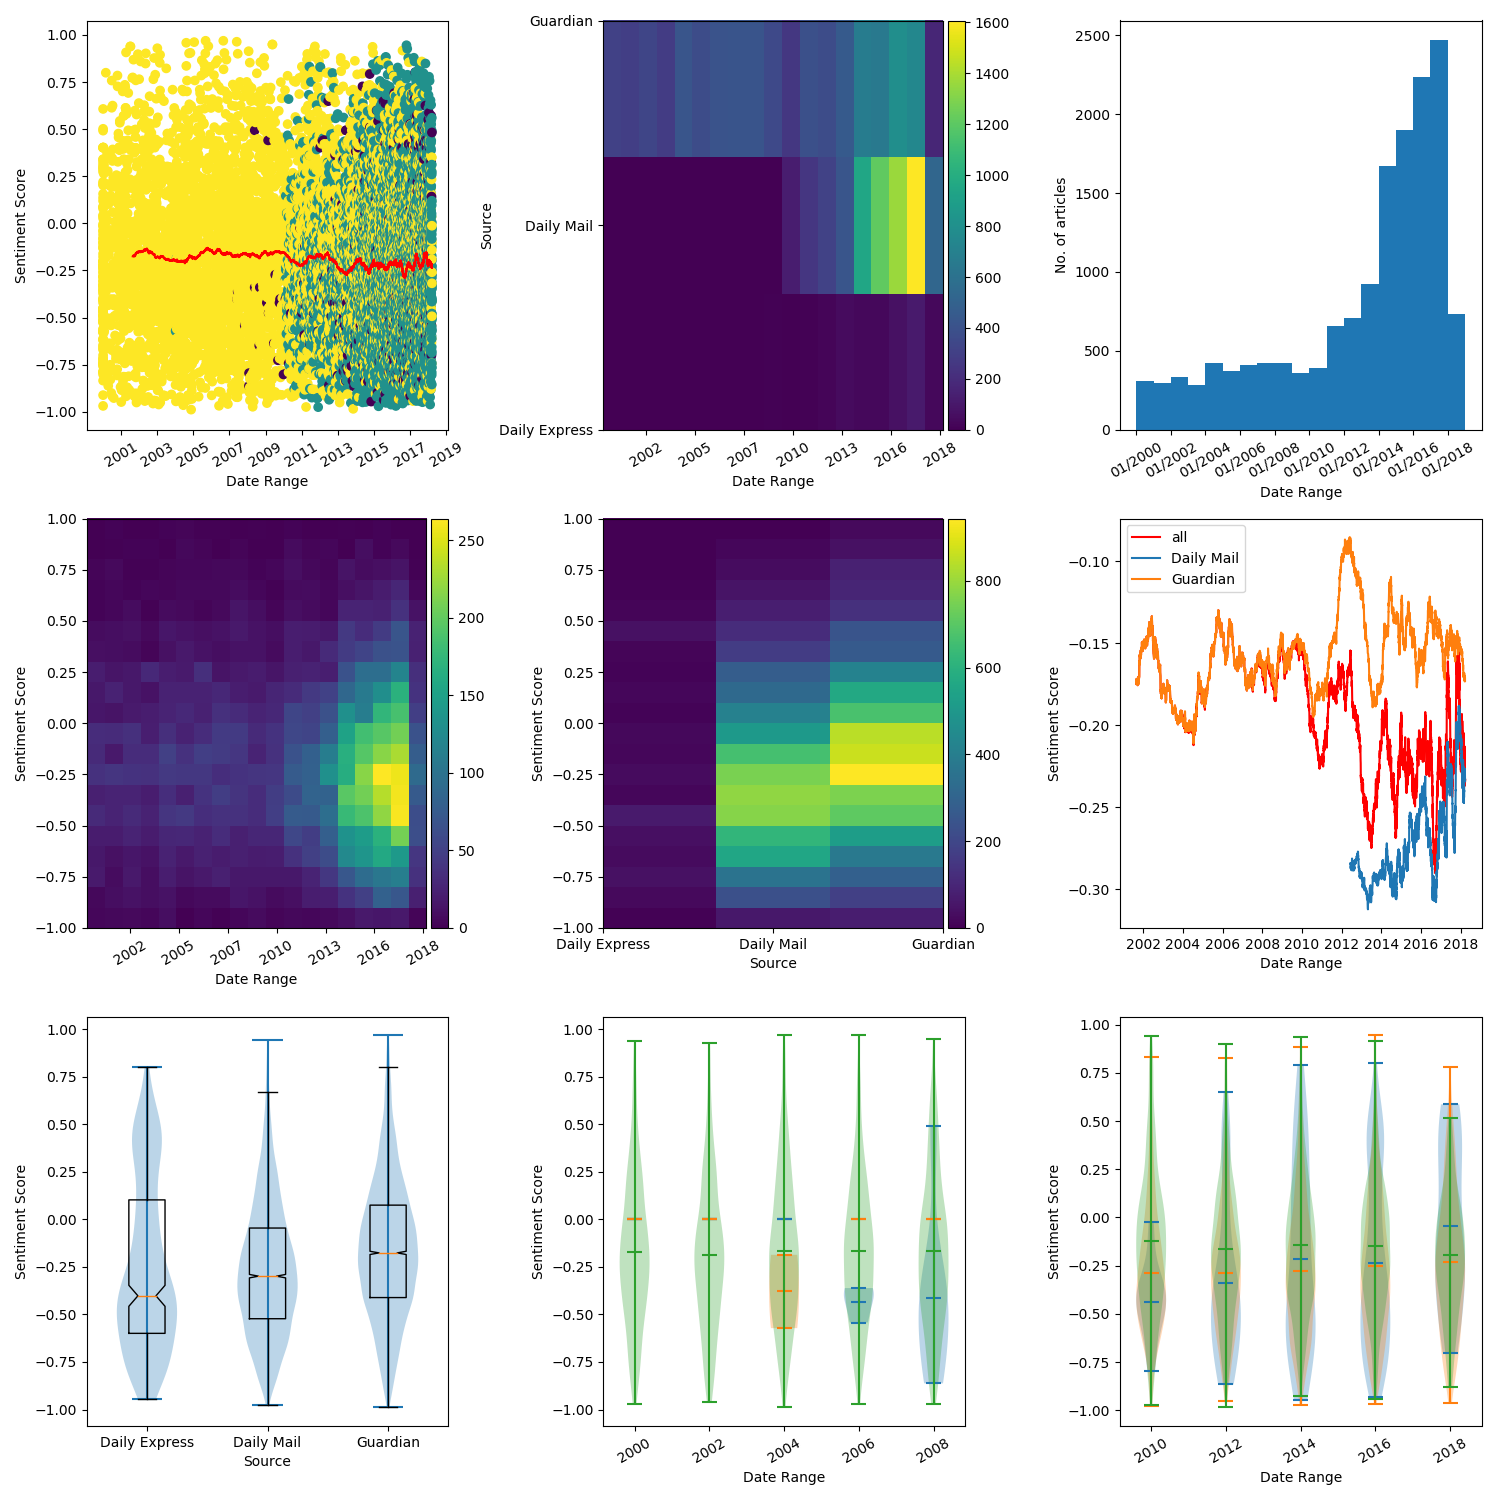
\includegraphics[width=\textwidth]{raw/mental-illness.png}

\subsection{Mann-Whitney $U$ Test Results ($p$-values)}
\noindent
\begin{tabu} to \textwidth { | X[c] | X[c] | X[c] | X[c] | }  
	\hline
	Topic & Guardian \textgreater\space Daily Mail & Guardian \textgreater\space Daily Express & Daily Express \textgreater\space Daily Mail  \\
	\hline
	All & 3.54 * 10\textsuperscript{-76} & 1.51 * 10\textsuperscript{-9} & 0.102 **  \\
	\hline
	2010 & 0.000255 & N/A & N/A  \\
	\hline
	2011 & 8.79 * 10\textsuperscript{-11} & N/A & N/A  \\
	\hline
	2012 & 5.70 * 10\textsuperscript{-8} & 0.377 & 0.112  \\
	\hline
	2013 & 1.13 * 10\textsuperscript{-7} & 1.43 * 10\textsuperscript{-7} & 0.000132 **  \\
	\hline
	2014 & 1.19 * 10\textsuperscript{-22} & 0.108 & 0.178  \\
	\hline
	2015 & 2.77 * 10\textsuperscript{-10} & 0.0588 & 0.401 **  \\
	\hline
	2016 & 1.83 * 10\textsuperscript{-19} & 2.56 * 10\textsuperscript{-11} & 2.03 * 10\textsuperscript{-5} **  \\
	\hline
	2017 & 5.55 * 10\textsuperscript{-10} & 0.389 ** & 0.00826  \\
	\hline
	2018* & 0.0531 & 0.0413 ** & 0.00878  \\
	\hline
\end{tabu}

\noindent * 2018 data is incomplete and would only include articles up to (approximately) end of March.

\noindent ** Indicates where the reverse assumption is true (e.g. Daily Mail \textgreater\space Daily Express instead of Daily Express \textgreater\space Daily Mail)

\subsection{Key Term Trend Plots}
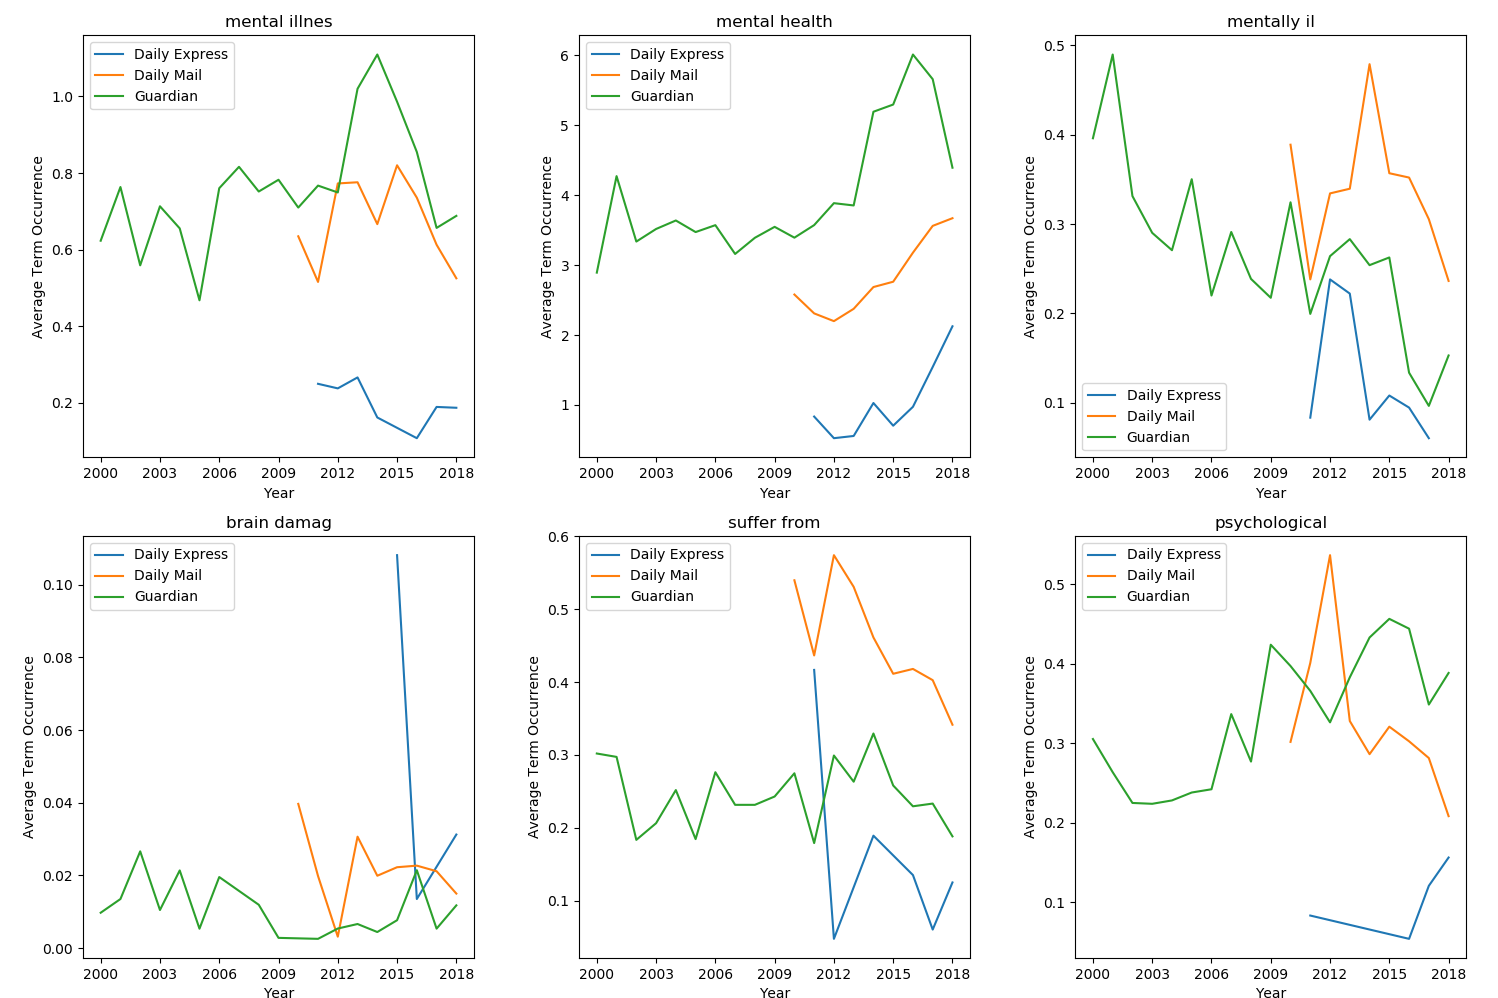
\includegraphics[width=\textwidth]{raw/mental-illness-terms.png}

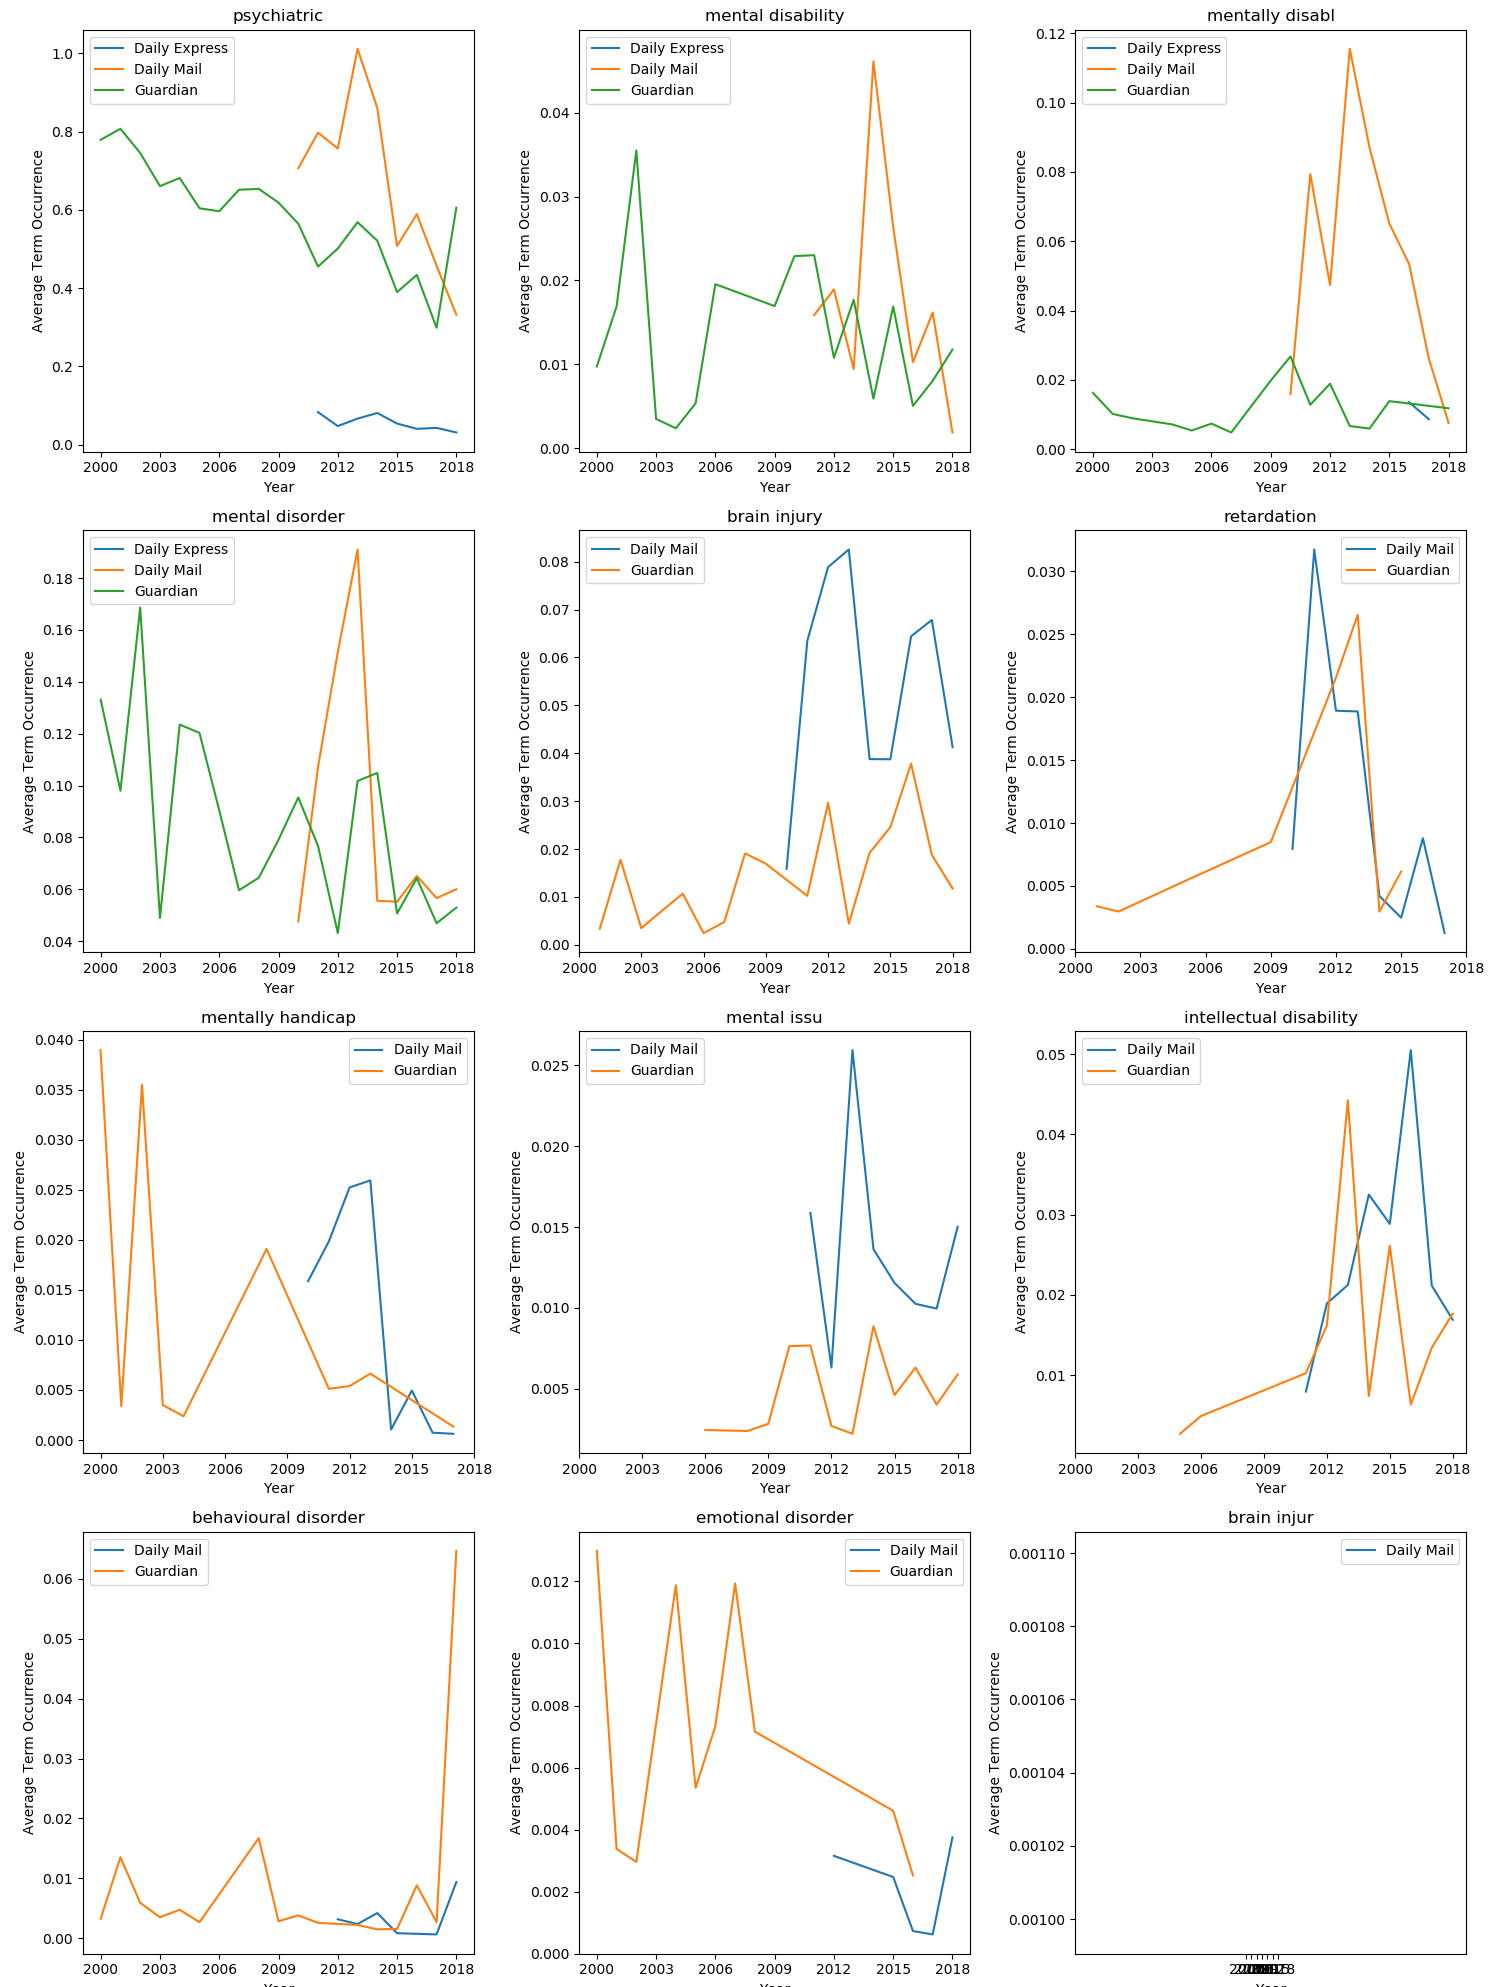
\includegraphics[width=\textwidth]{raw/mental-illness-terms2.png}

\newpage
\section{Topic: `mute'}
Key Terms: `mute', `muteness', `mutism', `cannot speak', `difficulty speaking', `synthetic speech', `non-vocal', `non-verbal'

\noindent Query Terms: `mute', `muteness', `mutism', `non-verbal'

\noindent Sample size, n = 456

\subsection{Sentiment Score Plots}
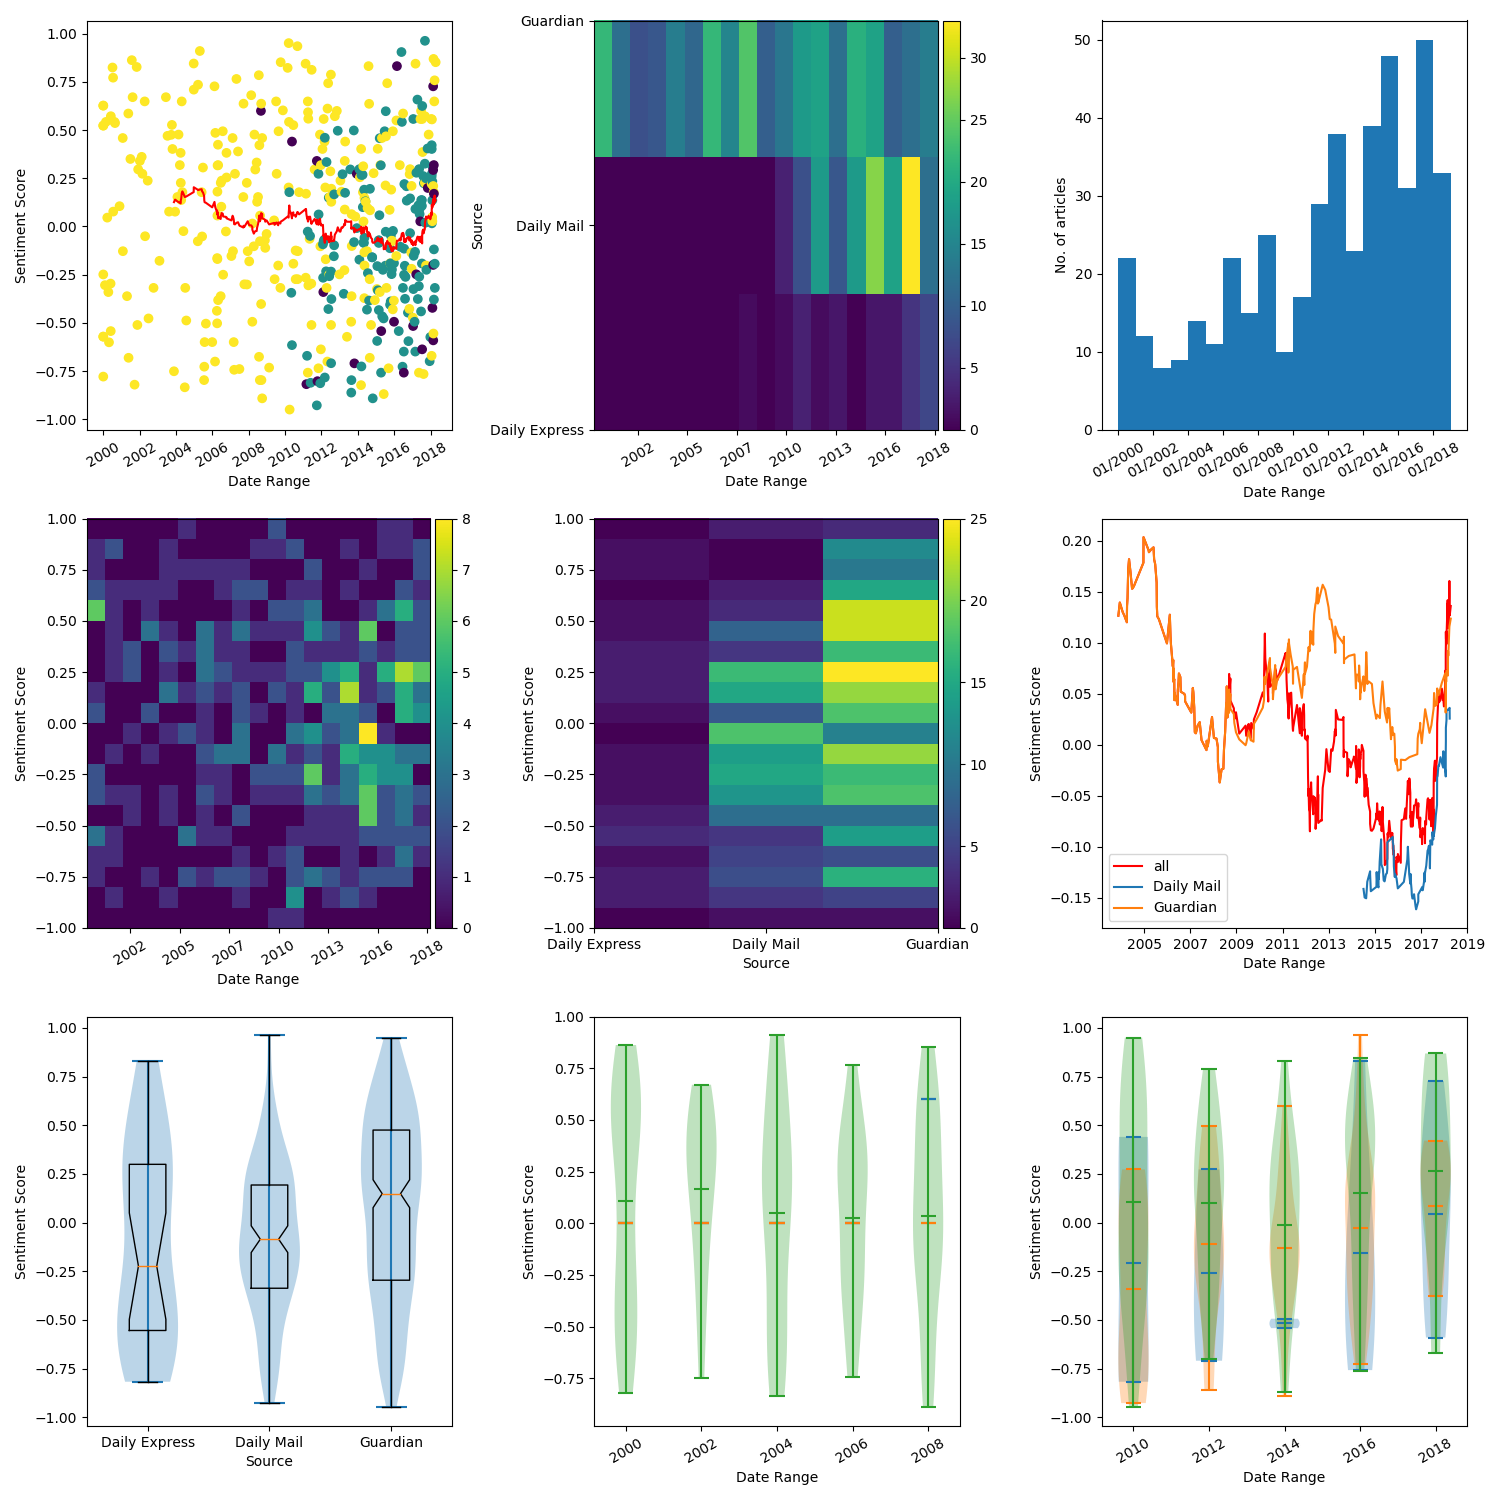
\includegraphics[width=\textwidth]{raw/mute.png}

\subsection{Mann-Whitney $U$ Test Results ($p$-values)}
\noindent
\begin{tabu} to \textwidth { | X[c] | X[c] | X[c] | X[c] | }  
	\hline
	Topic & Guardian \textgreater\space Daily Mail & Guardian \textgreater\space Daily Express & Daily Express \textgreater\space Daily Mail  \\
	\hline
	All & 6.78 * 10\textsuperscript{-5} & 0.0311 & 0.346 **  \\
	\hline
\end{tabu}

\noindent Insufficient sample size for year-by-year comparisons. (n=456).

\noindent ** Indicates where the reverse assumption is true (e.g. Daily Mail \textgreater\space Daily Express instead of Daily Express \textgreater\space Daily Mail)

\subsection{Key Term Trend Plots}
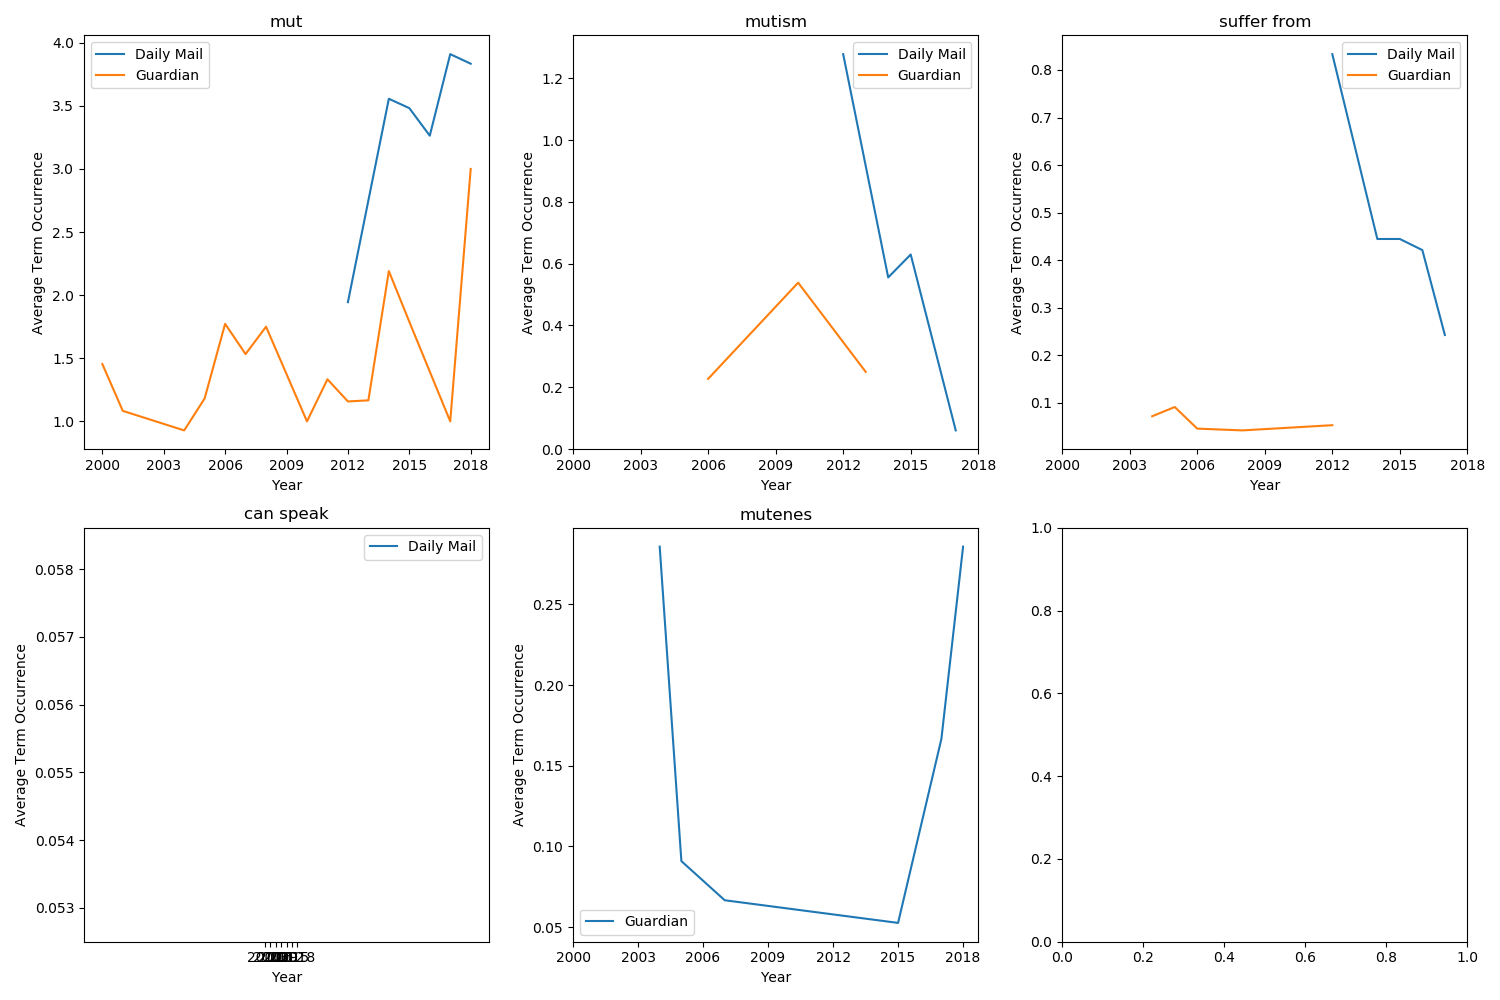
\includegraphics[width=\textwidth]{raw/mute-terms.png}

\newpage
\section{Topic: `paralysis'}
Key Terms: `paraplegic', `quadriplegic', `spinal cord', `paraplegia', `quadriplegia', `paralysed', `paralyzed', `paralysis', `crippled', `leg braces', `wheelchair'

\noindent Query Terms: `paraplegic', `quadriplegic', `paraplegia', `quadriplegia', `paralysis'

\noindent Sample size, n = 1,461

\subsection{Sentiment Score Plots}
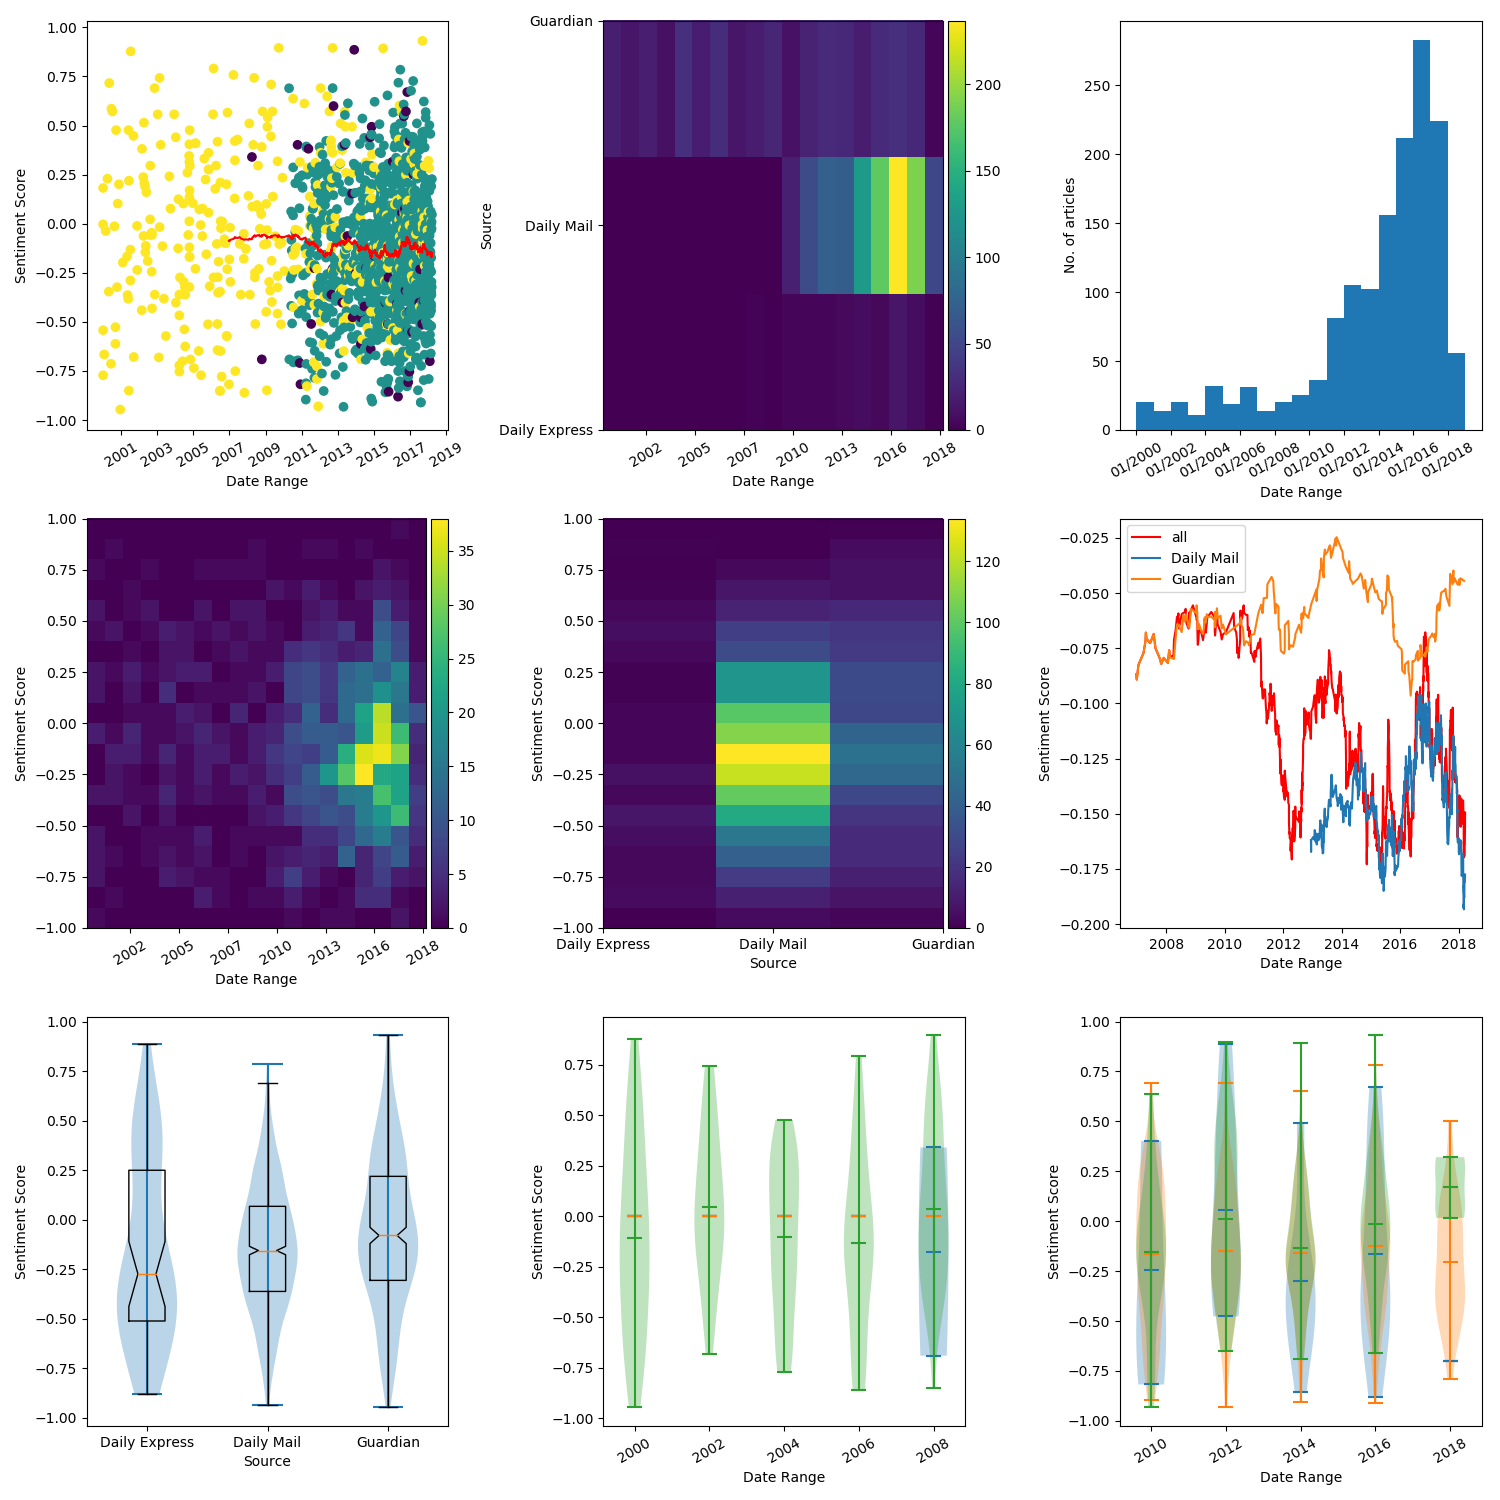
\includegraphics[width=\textwidth]{raw/paralysis.png}

\subsection{Mann-Whitney $U$ Test Results ($p$-values)}
\noindent
\begin{tabu} to \textwidth { | X[c] | X[c] | X[c] | X[c] | }
	\hline
	Topic & Guardian \textgreater\space Daily Mail & Guardian \textgreater\space Daily Express & Daily Express \textgreater\space Daily Mail  \\
	\hline
	All & 2.73 * 10\textsuperscript{-5} & 0.00909 & 0.0827 **  \\
	\hline
	2011 & 0.352 ** & N/A & N/A  \\
	\hline
	2012 & 0.00184 & N/A & N/A  \\
	\hline
	2013 & 0.374 & N/A & N/A  \\
	\hline
	2014 & N/A & N/A & N/A  \\
	\hline
	2015 & 0.331 & N/A & N/A  \\
	\hline
	2016 & 0.149 & N/A & N/A  \\
	\hline
	2017 & 0.00431 & N/A & N/A  \\
	\hline
\end{tabu}

\noindent ** Indicates where the reverse assumption is true (e.g. Daily Mail \textgreater\space Daily Express instead of Daily Express \textgreater\space Daily Mail)

\subsection{Key Term Trend Plots}
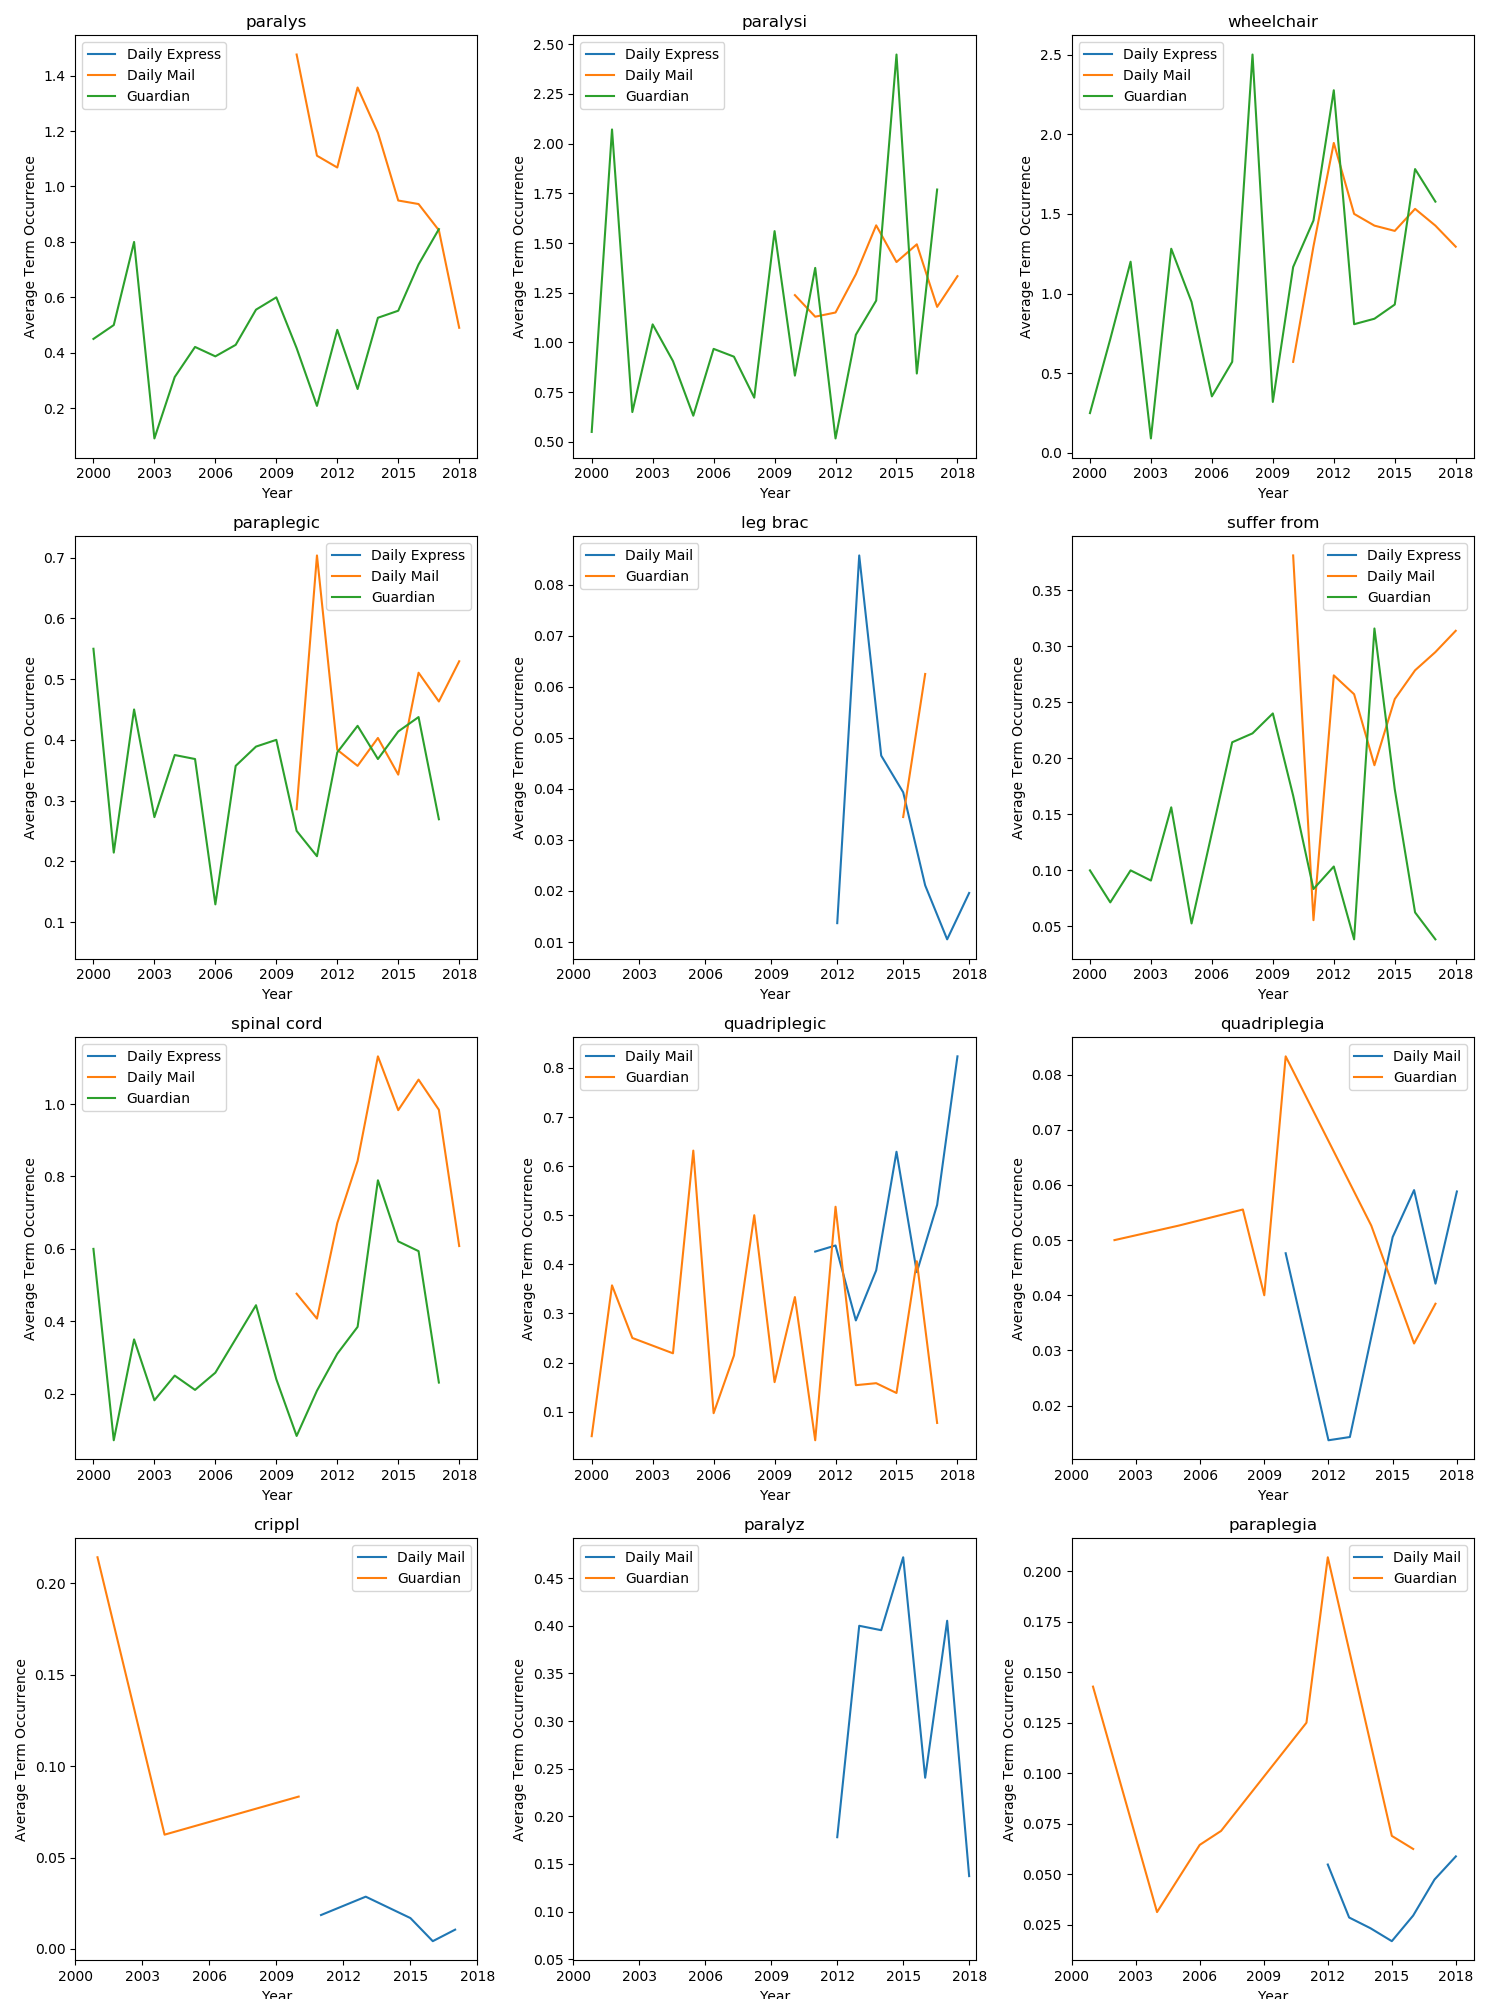
\includegraphics[width=\textwidth]{raw/paralysis-terms.png}

\newpage
\section{Topic: `speech impairment'}
Key Terms: `speech impairment', `stutter', `speech disability', `speech disorder', `communication disability', `difficulty speaking', `language impairment', `language disorder', `language disability', `speech impediment', `stammer'

\noindent Query Terms: `speech impairment', `stutter', `speech disorder', `speech impediment'

\noindent Sample size, n = 215

\subsection{Sentiment Score Plots}
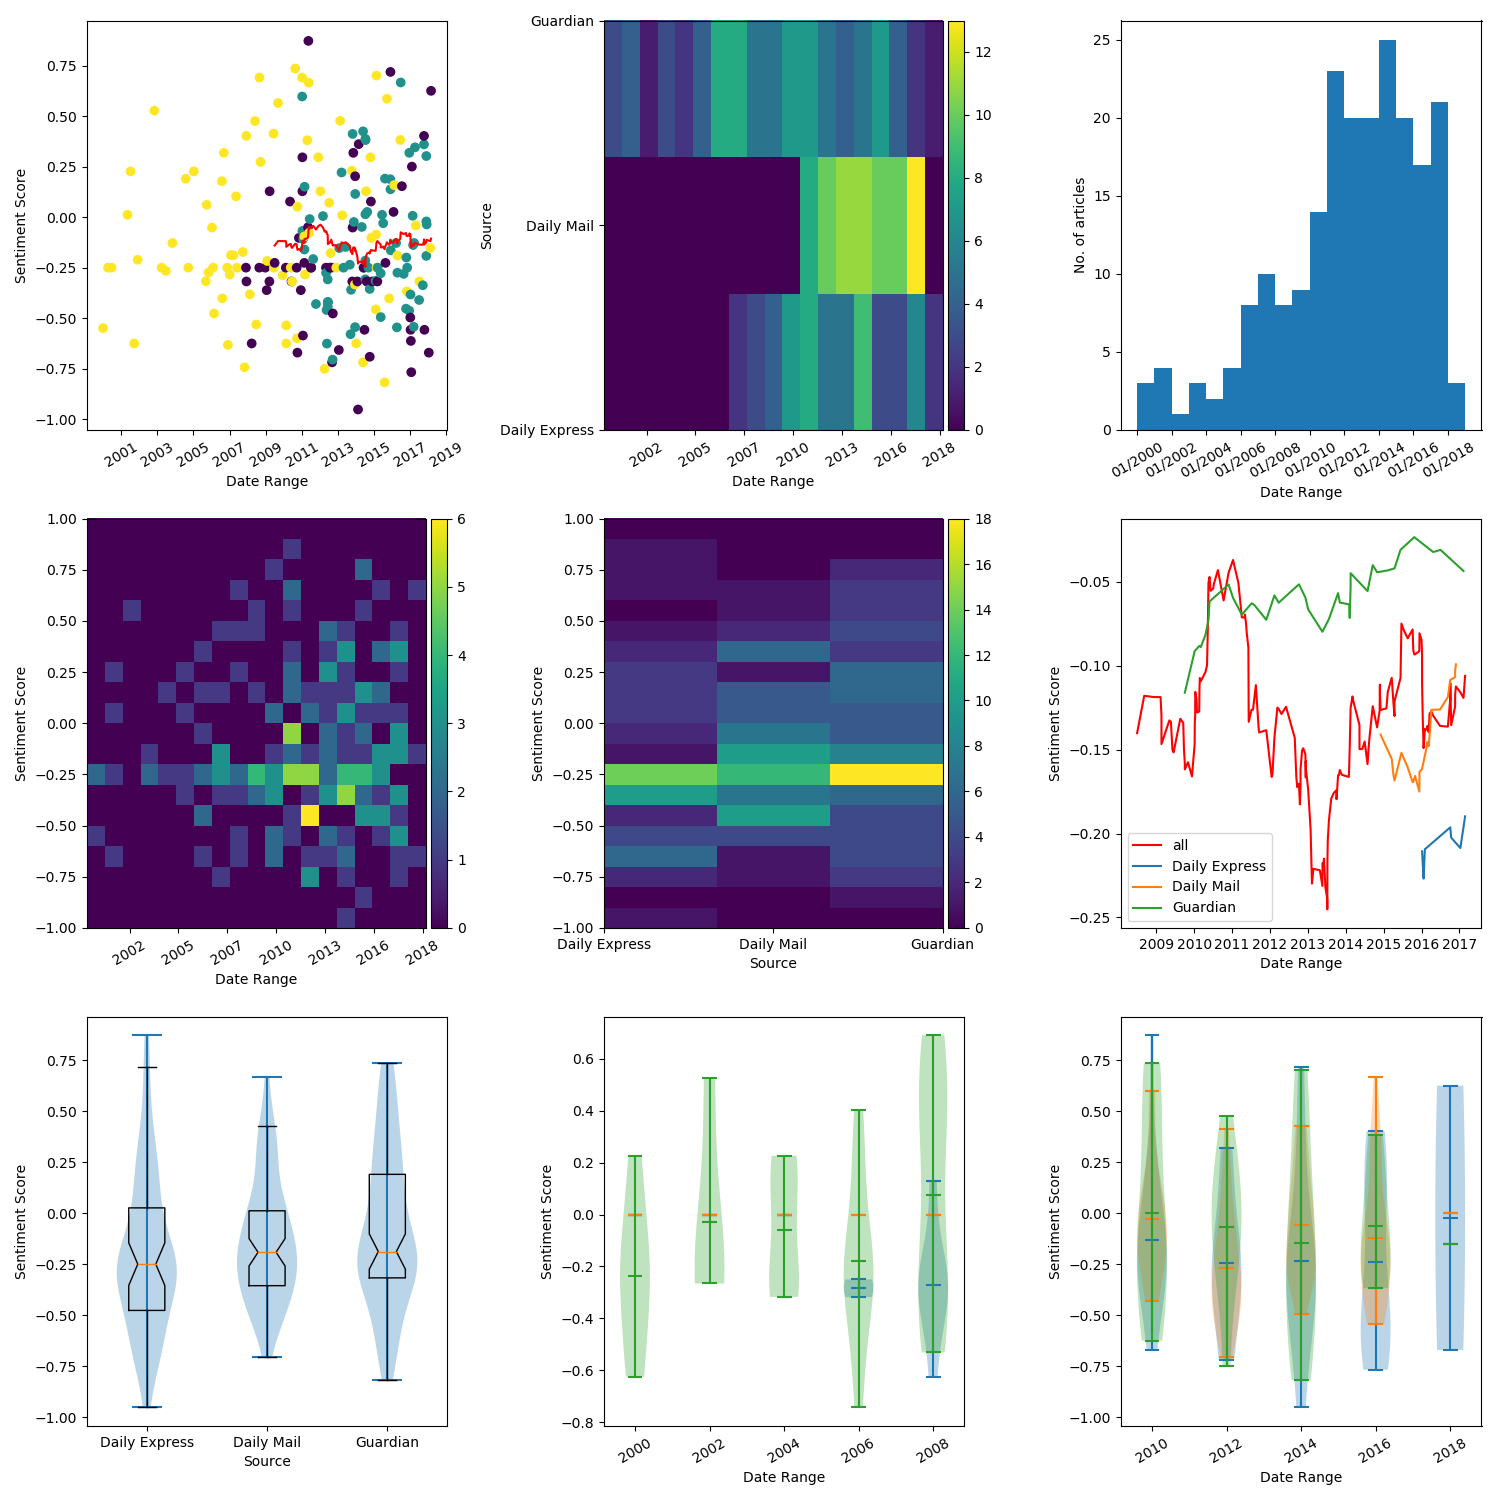
\includegraphics[width=\textwidth]{raw/speech-impairment.png}

\subsection{Mann-Whitney $U$ Test Results ($p$-values)}
\noindent
\begin{tabu} to \textwidth { | X[c] | X[c] | X[c] | X[c] | }
	\hline
	Topic & Guardian \textgreater\space Daily Mail & Guardian \textgreater\space Daily Express & Daily Express \textgreater\space Daily Mail  \\
	\hline
	All & 0.235 & 0.0200 & 0.0546 **  \\
	\hline
\end{tabu}

\noindent Insufficient sample size for year-by-year comparisons. (n=215).

\noindent ** Indicates where the reverse assumption is true (e.g. Daily Mail \textgreater\space Daily Express instead of Daily Express \textgreater\space Daily Mail)

\subsection{Key Term Trend Plots}
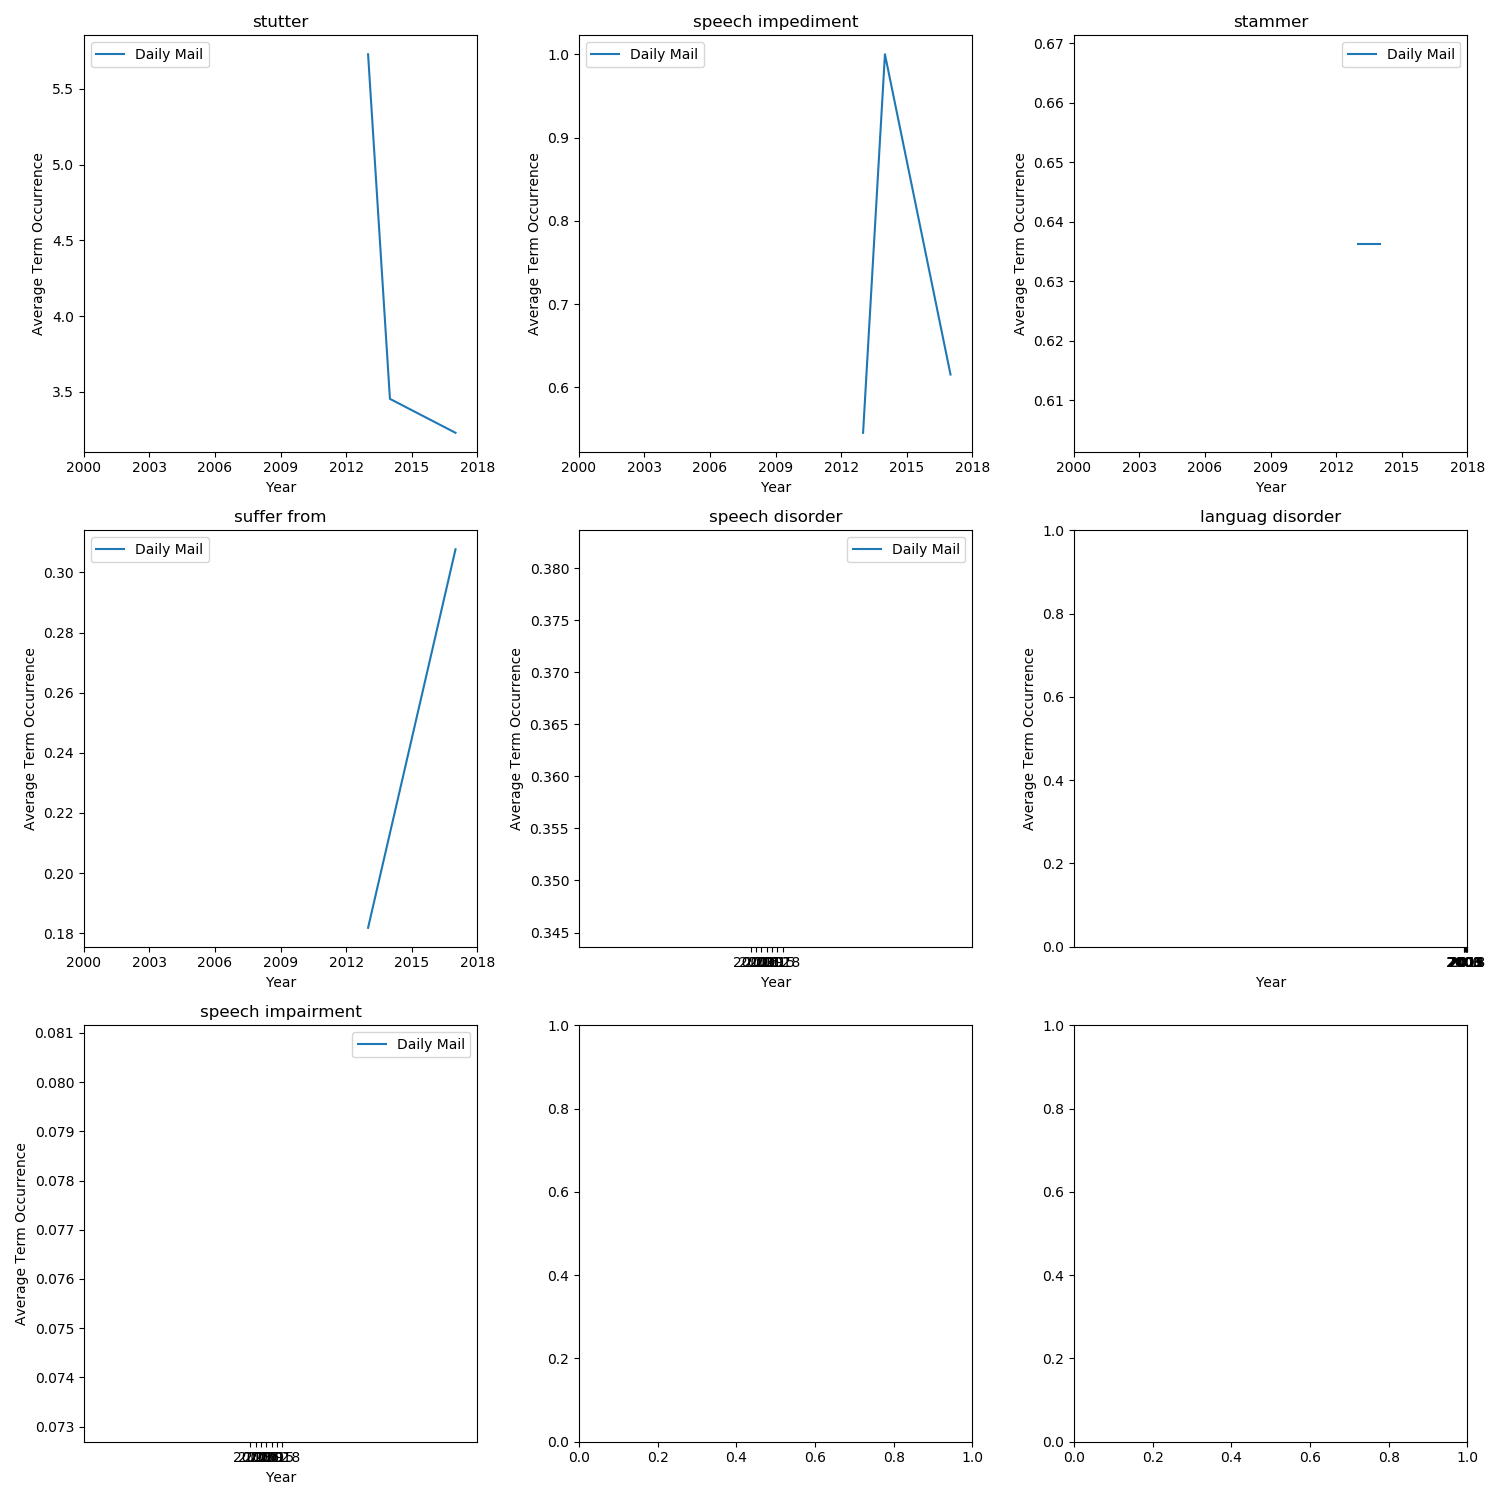
\includegraphics[width=\textwidth]{raw/speech-impairment-terms.png}

% \chapter{Test Appendix B}

\end{document}